\documentclass{article}


% if you need to pass options to natbib, use, e.g.:
%     \PassOptionsToPackage{numbers, compress}{natbib}
% before loading neurips_2024


% ready for submission
% \usepackage{neurips_2024}


% to compile a preprint version, e.g., for submission to arXiv, add add the
% [preprint] option:
% \usepackage[preprint]{neurips_2024}


% to compile a camera-ready version, add the [final] option, e.g.:
\usepackage[final]{neurips_2024}


% to avoid loading the natbib package, add option nonatbib:
%    \usepackage[nonatbib]{neurips_2024}


\usepackage[utf8]{inputenc} % allow utf-8 input
\usepackage[T1]{fontenc}    % use 8-bit T1 fonts
\usepackage{hyperref}       % hyperlinks
\usepackage{url}            % simple URL typesetting
\usepackage{booktabs}       % professional-quality tables
\usepackage{amsfonts}       % blackboard math symbols
\usepackage{nicefrac}       % compact symbols for 1/2, etc.
\usepackage{microtype}      % microtypography
\usepackage{xcolor}         % colors

%%%%%%%%%%%%%%%%%%%%%%%%%%%%%%%%%%%%%%%%%%%%%%%%%%%%%%%%%%%% Added by us
% Custom Bibliography
\setcitestyle{square,numbers,comma,sort&compress}
%\usepackage[sort&compress]{natbib}
\citestyle{plain}
\bibliographystyle{unsrtnat}

% Custom Packages (remove unnecessary ones)
\usepackage{graphicx}
\usepackage{float}
\usepackage{cancel}
\usepackage{color,soul}
\usepackage{mathtools}
\usepackage{wrapfig}
\usepackage{amssymb}
\usepackage{array}
\usepackage{tabularx}
\usepackage{makecell}
\usepackage[ruled,vlined]{algorithm2e}
\usepackage{bbold}
\usepackage{amsthm}
\usepackage{caption}
\usepackage{subcaption}
\usepackage{paralist}
\usepackage{multirow}
\usepackage{booktabs}
\usepackage[capitalise]{cleveref}

% Custom theorem environments
\theoremstyle{plain}
\newtheorem{theorem}{Theorem}[section]
\newtheorem{proposition}[theorem]{Proposition}
\newtheorem{lemma}[theorem]{Lemma}
\newtheorem{corollary}[theorem]{Corollary}
\theoremstyle{definition}
\newtheorem{definition}[theorem]{Definition}
\newtheorem{assumption}[theorem]{Assumption}
\theoremstyle{remark}
\newtheorem{remark}[theorem]{Remark}
\newtheorem{conjecture}[theorem]{Conjecture}

% Custom math operators
\DeclareMathOperator*{\argmax}{arg\,max}
\DeclareMathOperator*{\argmin}{arg\,min}
\DeclareMathOperator{\rank}{rank}

% Title
\title{Get rich quick: exact solutions reveal how unbalanced initializations promote rapid feature learning}


% Authors
\usepackage{authblk}
\makeatletter
\renewcommand\AB@affilsepx{ \quad \protect\Affilfont}
\def\thanks#1{\protected@xdef\@thanks{\@thanks\protect\footnotetext{#1}}}
\makeatother
\def\Authsep{\quad}
\def\Authands{\quad}

\author[1]{\bf Daniel Kunin$^*$\thanks{$^*$ Equal contribution. Correspondence to \texttt{kunin@stanford.edu} and \texttt{aravento@stanford.edu}.}}
\author[1]{\bf Allan Raventós$^*$}
\author[2]{\bf Clémentine Dominé}
\author[1]{\bf Feng Chen}
\author[3]{\\ \bf David Klindt}
\author[2]{\bf Andrew Saxe}
\author[1]{\bf Surya Ganguli}
\affil[1]{Stanford University}
\affil[2]{University College London}
\affil[3]{Cold Spring Harbor Laboratory}



%%%%%%%%%%%%%%%%%%%%%%%%%%%%%%%%%%%%%%%%%%%%%%%%%%%%%%%%%%%%
\begin{document}


\maketitle

% TLDR
% We derive exact solutions to a minimal model that transitions between lazy and rich learning, precisely elucidating how unbalanced \emph{layer-specific} initialization variances and learning rates determine the degree of feature learning in a finite-width network.

\begin{abstract}
    \vspace{-10pt}
    While the impressive performance of modern neural networks is often attributed to their capacity to efficiently extract task-relevant features from data, the mechanisms underlying this \emph{rich feature learning regime} remain elusive, with much of our theoretical understanding stemming from the opposing \emph{lazy regime}.
    %
    In this work, we derive exact solutions to a minimal model that transitions between lazy and rich learning, precisely elucidating how unbalanced \emph{layer-specific} initialization variances and learning rates determine the degree of feature learning. % in a finite-width network.
    %
    % they = initialization variances and learning rates
    Our analysis reveals that they conspire to influence the learning regime through a set of conserved quantities that constrain and modify the geometry of learning trajectories in parameter and function space.
    %
    We extend our analysis to more complex linear models with multiple neurons, outputs, and layers and to shallow nonlinear networks with piecewise linear activation functions.
    % 
    In linear networks, rapid feature learning only occurs from balanced initializations, where all layers learn at similar speeds. 
    %
    While in nonlinear networks, unbalanced initializations that promote faster learning in earlier layers can accelerate rich learning.
    %
    Through a series of experiments, we provide evidence that this unbalanced rich regime drives feature learning in deep finite-width networks, promotes interpretability of early layers in CNNs, reduces the sample complexity of learning hierarchical data, and decreases the time to grokking in modular arithmetic. 
    %
    Our theory motivates further exploration of unbalanced initializations to enhance efficient feature learning.% in deep neural networks.
\end{abstract}


%%%%%%%%%%%%%%%%%%%%%%%%%%%%%%%%%%%%%%%%%%%%%%%%%%%%%%%%%%%%
\vspace{-10pt}
\section{Introduction}
\label{sec:introduction}
\vspace{-5pt}



Deep learning has transformed machine learning, demonstrating remarkable capabilities in a myriad of tasks ranging from image recognition to natural language processing. 
% 
It's widely believed that the impressive performance of these models lies in their capacity to efficiently extract task-relevant features from data.
%
However, understanding this feature acquisition requires unraveling a complex interplay between datasets, network architectures, and optimization algorithms.
%
Within this framework, two distinct regimes, determined at initialization, have emerged: the lazy and the rich.


\textbf{Lazy regime.} 
Various investigations have revealed a notable phenomenon in overparameterized neural networks, where throughout training the networks remain close to their linearization \cite{du2018gradient, du2019gradient, allen2019learning, allen2019convergence, zou2020gradient}.
%
Seminal work by \citet{jacot2018neural}, demonstrated that in the infinite-width limit, the Neural Tangent Kernel (NTK), which describes the evolution of the neural network through training, converges to a deterministic limit.
%
Consequently, the network learns a solution akin to kernel regression with the NTK matrix.
%
Termed the \emph{lazy} or \emph{kernel} regime, this domain has been characterized by a deterministic NTK \cite{jacot2018neural, yang2020tensor}, minimal movement in parameter space \cite{chizat2019lazy}, static hidden representations, exponential learning curves, and implicit biases aligned with a reproducing kernel Hilbert space (RKHS) norm \cite{azulay2021implicit}.
%
However, \citet{chizat2019lazy} challenged this understanding, asserting that the lazy regime isn't a product of the infinite-width architecture, but is contingent on the $\emph{overall scale}$ of the network at initialization.
%
They demonstrated that given any finite-width model $f(x;\theta)$ whose output is zero at initialization, a scaled version of the model $\tau f(x;\theta)$ will enter the lazy regime as the scale $\tau$ diverges.
%
However, they also noted that these scaled models often perform worse in test error.
%
While the lazy regime offers insights into the network's convergence to a global minimum, it does not fully capture the generalization capabilities of neural networks trained with standard initializations.
%
It is thus widely believed that a different regime, driven by small or vanishing initializations, underlies the many successes of neural networks.



\textbf{Rich regime.}
%
In contrast to the lazy regime, the \emph{rich} or \emph{feature-learning} or \emph{active} regime is distinguished by a learned NTK that evolves through training, non-convex dynamics traversing between saddle points \cite{saxe2013exact, saxe2019mathematical,jacot2021saddle}, sigmoidal learning curves, and simplicity biases such as low-rankness \cite{li2020towards} or sparsity \cite{woodworth2020kernel}.
%
Yet, the exact characterization of rich learning and the features it learns frequently depends on the specific problem at hand, with its definition commonly simplified as what it is not: lazy.
%
Recent analyses have shown that beyond overall scale, other aspects of the initialization can substantially impact the extent of feature learning, such as the effective rank \cite{liu2023connectivity}, layer-specific initialization variances \cite{yang2020feature, luo2021phase, yang2022tensor}, and large learning rates \cite{lewkowycz2020large, ba2022high, zhu2023catapults, cui2024asymptotics}. 
%
\citet{azulay2021implicit} demonstrated that in two-layer linear networks, the relative difference in weight magnitudes between the first and second layer, termed the \emph{relative scale} in our work, can impact feature learning, with balanced initializations yielding rich learning dynamics, while unbalanced ones tend to induce lazy dynamics.
%
However, as shown in \cref{fig:two-layer-relu}, for nonlinear networks unbalanced initializations can induce both rich and lazy dynamics,  creating a complex phase portrait of learning regimes influenced by both overall and relative scale.
%
Building on these observations, our study aims to precisely understand how layer-specific initialization variances and learning rates determine the transition between lazy and rich learning in finite-width networks.
%
Moreover, we endeavor to gain insights into the inductive biases of both regimes, and the transition between them, during training and at interpolation, with the ultimate goal of elucidating how the rich regime acquires features that facilitate generalization.



\begin{figure*}[t]
    \begin{subfigure}[c]{0.465\textwidth}
        \label{fig:two-layer-relu-a}
        \centering
        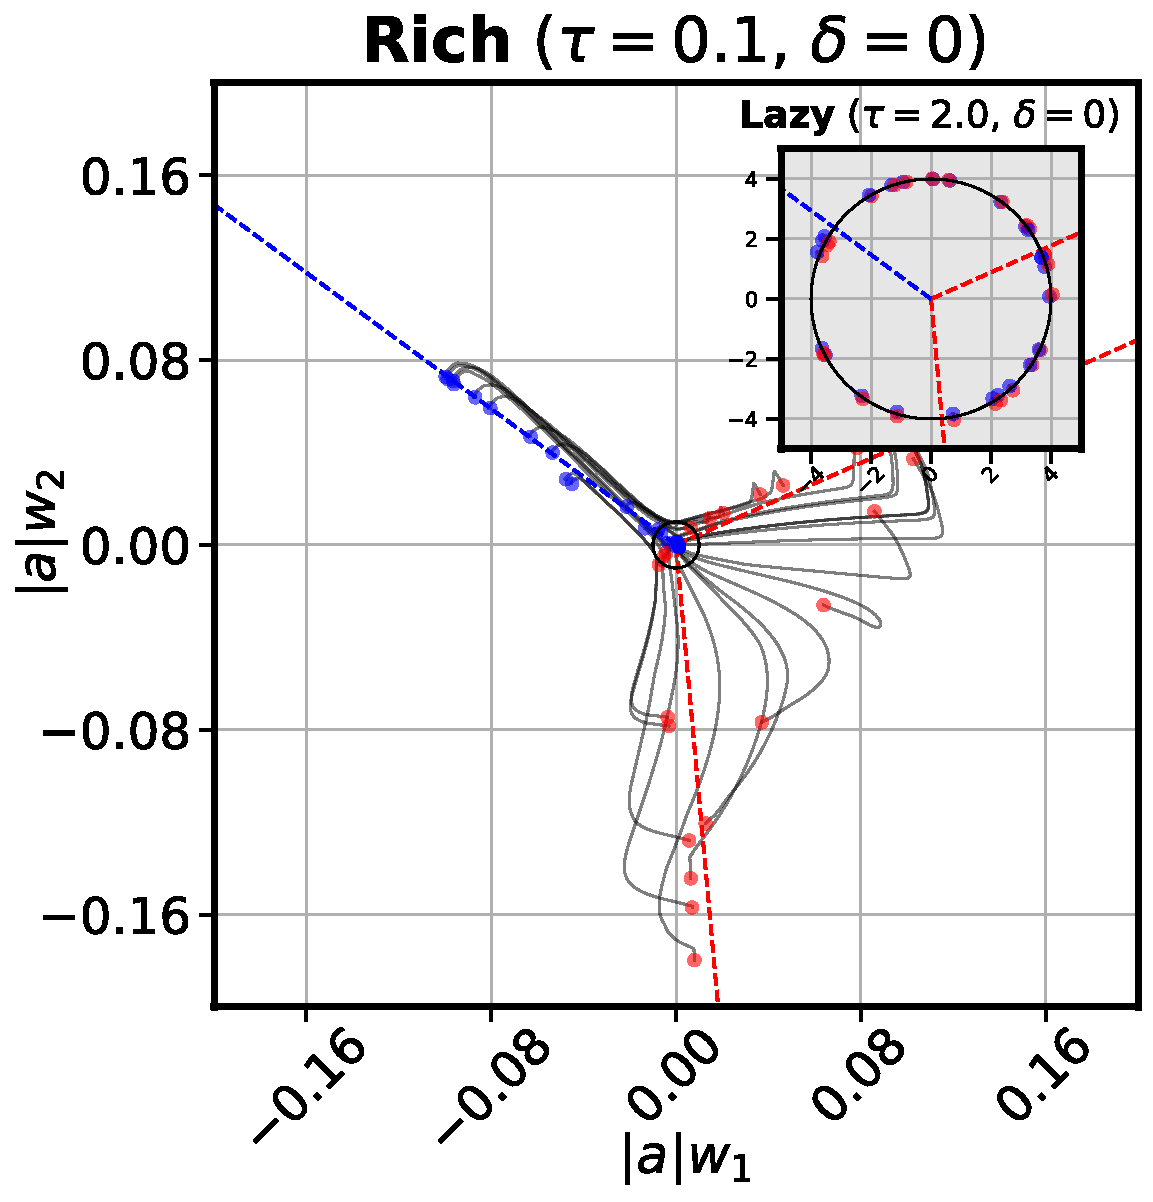
\includegraphics[width=0.49\linewidth]{fig/two-layer/scale.pdf}
        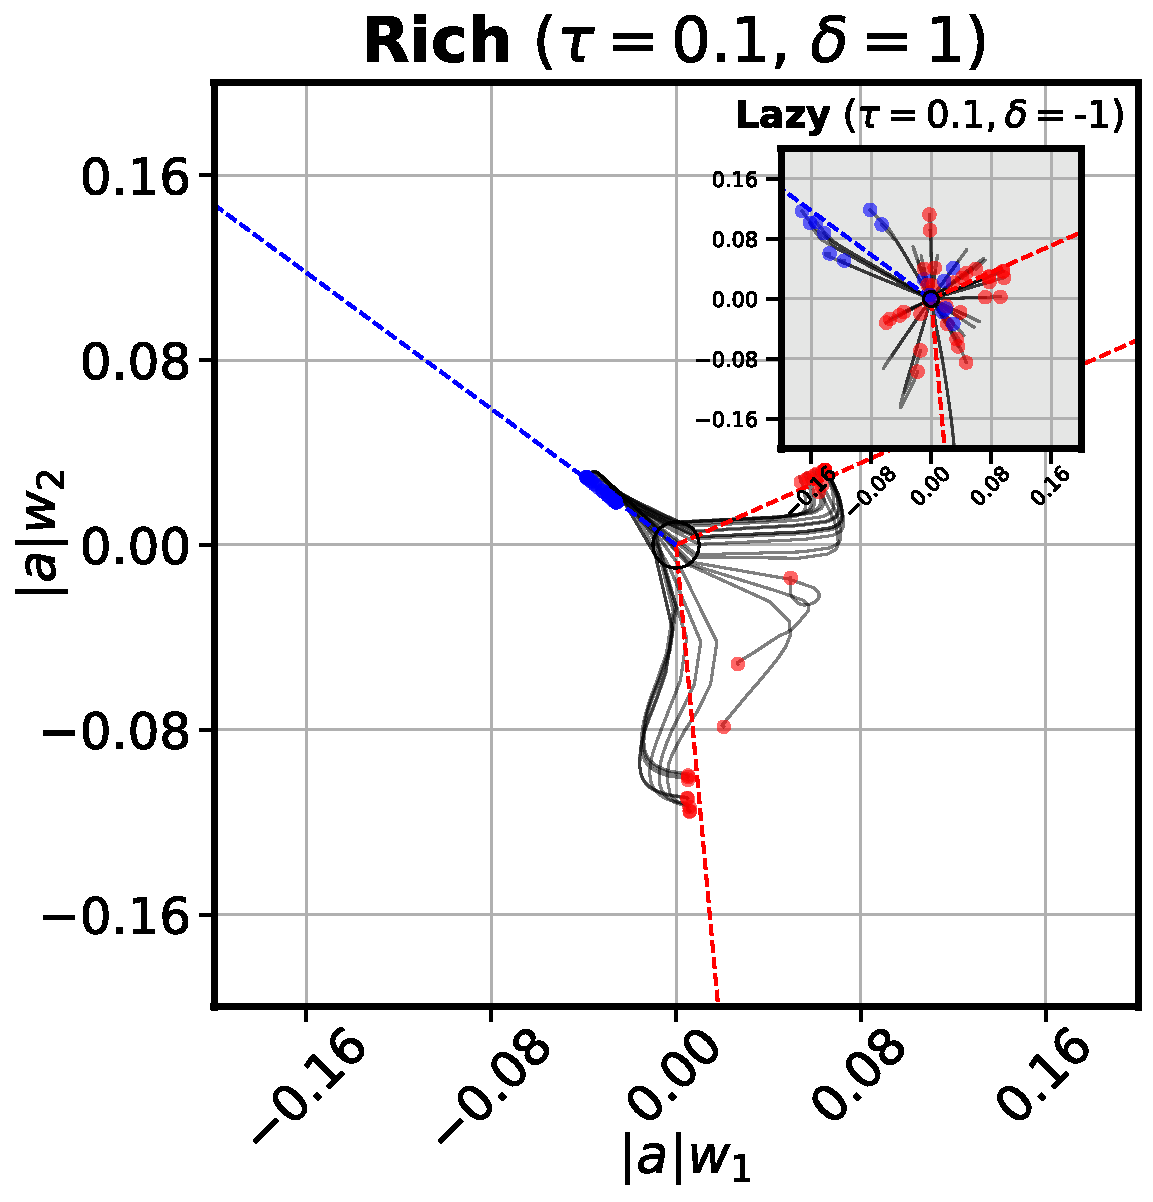
\includegraphics[width=0.49\linewidth]{fig/two-layer/shape.pdf}
        \caption{Overall and relative scale impact feature learning}
    \end{subfigure}
    \begin{subfigure}[c]{0.53\textwidth}
        \label{fig:two-layer-relu-b}
        \centering
        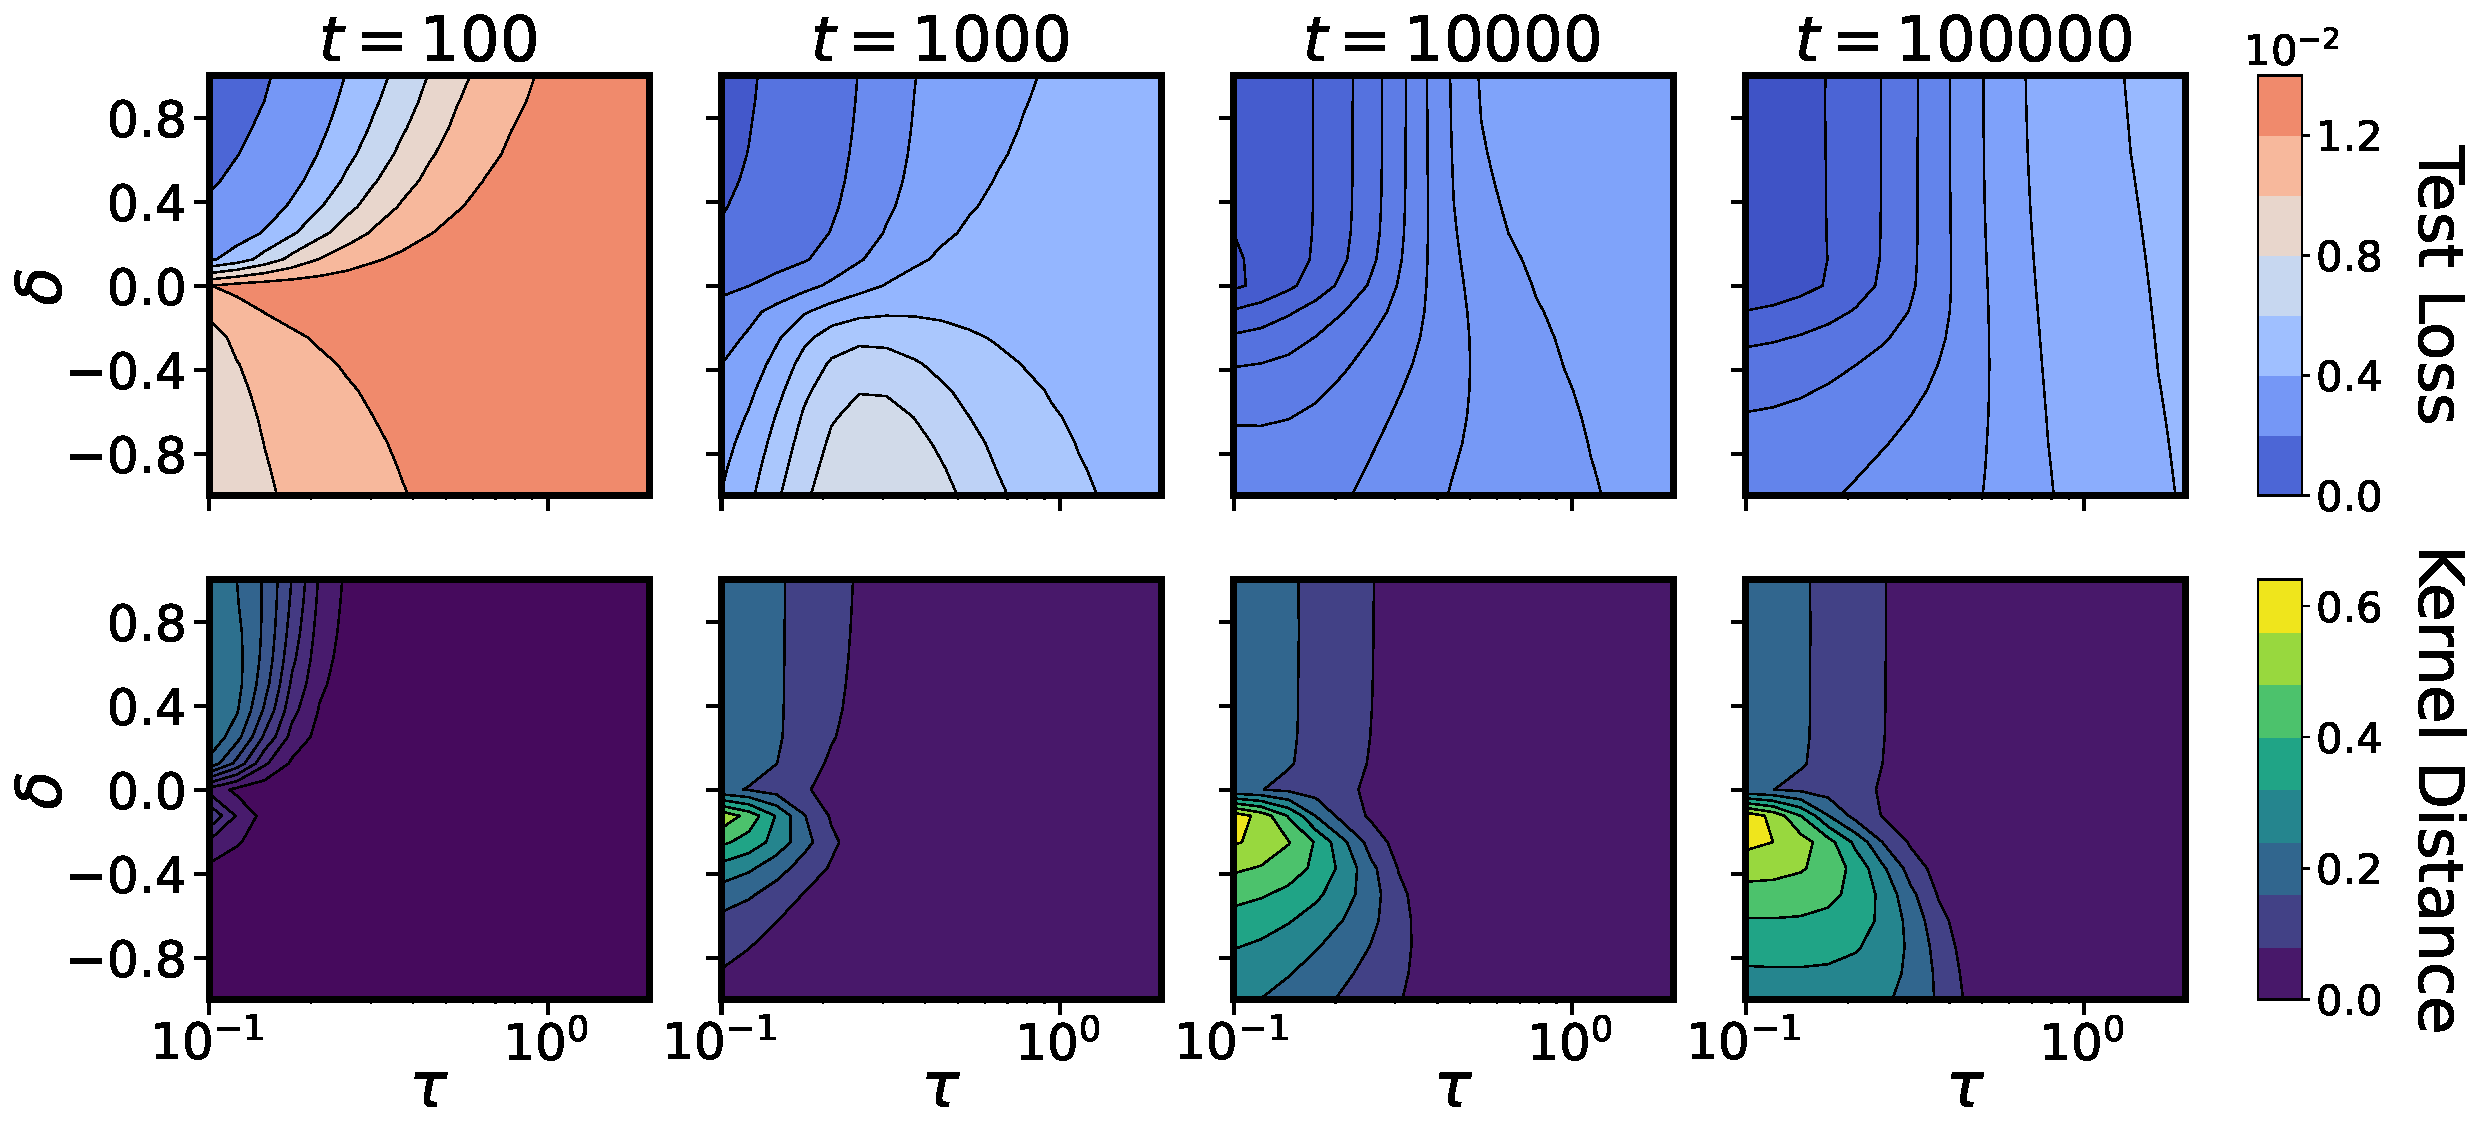
\includegraphics[width=\linewidth]{fig/two-layer/test_loss_and_kernel_distance.pdf}
        \caption{A complex phase portrait of feature learning}
    \end{subfigure}
    \caption{\textbf{Unbalanced initializations lead to rapid rich learning and generalization.}
    %
    We follow the experimental setup used in Fig. 1 of \citet{chizat2019lazy} -- a wide two-layer student ReLU network $f(x;\theta) = \sum_{i=1}^h a_i \max(0,w_i^\intercal x)$ trained on a dataset generated from a narrow two-layer teacher ReLU network.
    %
    The student parameters are initialized as $w_i \sim \text{Unif}(\mathbb{S}^{d-1}(\frac{\tau}{\alpha}))$ and $a_i = \pm\alpha\tau$, such that $\tau > 0$ controls the \emph{overall scale} of the function, while $\alpha > 0$ controls the \emph{relative scale} of the first and second layers through the conserved quantity $\delta = \tau^2 (\alpha^2 - \alpha^{-2})$.
    %
    (a) Shows the training trajectories of $|a_i|w_i$ (color denotes $\mathrm{sgn}(a_i)$) when $d = 2$ for four different settings of $\tau, \delta$.
    %
    The left plot confirms that small overall scale leads to rich and large overall scale to lazy.
    %
    The right plot shows that even at small overall scale, the relative scale can move the network between rich and lazy as well.
    %
    Here an upstream initialization $\delta > 0$ shows striking alignment to the teacher (dotted lines), while a downstream initialization $\delta < 0$ shows no alignment.
    %
    (b) Shows the test loss and kernel distance from initialization computed through training over a sweep of $\tau$ and $\delta$ when $d=100$.
    %
    Lazy learning happens when $\tau$ is large, rich learning happens when $\tau$ is small, and rapid rich learning happens when \emph{both} $\tau$ is small and $\delta$ is large -- an upstream initialization.
    %
    This initialization also leads to the smallest test loss.
    %
    See \cref{fig:two-layer-supporting} in \cref{app:experimental-details-two-layer} for supporting figures.
    }
    \label{fig:two-layer-relu}
    \vspace{-20pt}
\end{figure*}


\textbf{Our contributions.}
%
Our work begins with an exploration of the two-layer single-neuron linear network proposed by \citet{azulay2021implicit} as a minimal model displaying both lazy and rich learning.
%
In \cref{sec:single-neuron}, we derive exact solutions for the gradient flow dynamics with layer-specific learning rates of this model by employing a combination of hyperbolic and spherical coordinate transformations.
% By employing a combination of hyperbolic and spherical coordinate transformations, we derive in \cref{sec:single-neuron} exact solutions for the gradient flow dynamics with layer-specific learning rates under all initializations.
%
Alongside recent work by \citet{xu2024does}\footnote{\citet{xu2024does} presented exact NTK dynamics for a linear model trained with one-dimensional data.}, our analysis stands out as one of the few analytically tractable models for the transition between lazy and rich learning in a finite-width network, marking a notable contribution to the field.
%
% Our analysis reveals that the layer-specific initialization variances and learning rates, which we collectively refer to as the \emph{initialization geometry}, conspire to influence the learning regime through a simple set of conserved quantities that constrain the geometry of learning trajectories.
Our analysis reveals that the layer-specific initialization variances and learning rates conspire to influence the learning regime through a simple set of conserved quantities that constrain the geometry of learning trajectories.
% , which we refer to as the \emph{relative scale}. 
%
Additionally, it reveals that a crucial aspect of the relative scale overlooked in prior analysis is its directionality.
%
While a \emph{balanced initialization} results in all layers learning at similar rates, an \emph{unbalanced initialization} can cause faster learning in either earlier layers, referred to as an \emph{upstream initialization}, or later layers, referred to as a \emph{downstream initialization}. 
%
Due to the depth-dependent expressivity of layers in a network, upstream and downstream initializations often exhibit fundamentally distinct learning trajectories.
%
In \cref{sec:wide-deep-linear} we extend our analysis of the relative scale developed in the single-neuron model to more complex linear models with multiple neurons, outputs, and layers and in \cref{sec:nonlinear} to two-layer nonlinear networks with piecewise linear activation functions.
%
We find that in linear networks, rapid rich learning can only occur from balanced initializations, while in nonlinear networks, upstream initializations can actually accelerate rich learning.
%
Finally, through a series of experiments, we provide evidence that upstream initializations drive feature learning in deep finite-width networks, promote interpretability of early layers in CNNs, reduce the sample complexity of learning hierarchical data, and decrease the time to grokking in modular arithmetic.


%%%%%%%%%%%%%%%%%%%%%%%%
% DEFINITIONS
%%%%%%%%%%%%%%%%%%%%%%%%
% Initialization Geometry refers collectively to the layer-specific initialization variances and learning rates.  Has two features: overall scale and relative scale.

% Overall scale is the overall scale of the input-output map. Is either large or small.

% Relative scale is the relative scale between layers of the network. Has two classes "balanced" and "unbalanced":

%  - Balanced Initialization - All layers learning at similar rates (\delta = 0)

%  - Unbalanced Initialization - Layers learn at varying rates (\delta \neq 0).  Has two classes (for a two layer network) "upstream" and "downstream"
%       * Upstream Initialization - Early layers learn faster than latter layers (\delta > 0).
%       * Downstream Initialization - Latter layers learn faster than earlier layers (\delta < 0).

%%%%%%%%%%%%%%%%%%%%%%%%
% NOTATION
%%%%%%%%%%%%%%%%%%%%%%%%
%%% Dimensions %%%
% d = input dimension
% c = output dimension
% n = number of training points
% m = number of parameters
% h = width of hidden layer
% L = number of hidden layers
% N = total number of hidden neurons (across network)

%%% Indexing %%%
% i, j, k, l, p = indices
% i, j prefered for indexing data
% k prefered for indexing neurons
% l prefered for indexing layers
% p prefered for indexing parameters

%%% Network %%%
% \theta is parameters
% x_i, y_i is input, output
% X, Y is input, output matrices
% f(x;\theta) is NN

%%% Optimization %%%
% \mathcal{L} is loss
% \eta is learning rate
% \lambda is regularization rate
% t is gradient flow time
% \Theta is NTK
% K is NTK matrix (over training data)
% something_t means something quanitity at that point in time


\textbf{Notation.}
%
In this work, we consider a feedforward network $f(x;\theta): \mathbb{R}^d \to \mathbb{R}^c$ parameterized by $\theta \in \mathbb{R}^m$.
%
Unless otherwise specified, $c = 1$.
%
The network is trained by gradient flow $\dot{\theta} = -{\eta_{\theta}} \cdot \nabla_{\theta} \mathcal{L}(\theta)$, with an initialization $\theta_0$ and layer-specific learning rate $\eta_{\theta} \in \mathbb{R}^m_+$, to minimize the mean squared error $\mathcal{L}(\theta) = \frac{1}{2} \sum_{i=1}^n (f(x_i;\theta) - y_i)^2$ computed over a dataset $\{(x_1,y_1),\dots,(x_n,y_n)\}$ of size $n$.
%
We denote the input matrix as $X \in \mathbb{R}^{n \times d}$ with rows $x_i \in \mathbb{R}^d$ and the label vector as $y \in \mathbb{R}^n$.
%
% \footnote{Throughout this work we use the notation $\dot{x}$ and $\partial_t x$ interchangeably and we will often drop the explicit $t$ dependence on functions of the parameters $g(\theta) = g(\theta(t))$ or use the shorthand $g_t = g(\theta(t))$.}
%
The network's output $f(x;\theta)$ evolves according to the differential equation, $\partial_tf(x;\theta) = \sum_{i=1}^n \Theta(x,x_i;\theta)(y_i - f(x_i;\theta))$, where $\Theta(x,x';\theta) : \mathbb{R}^{d} \times \mathbb{R}^{d} \to \mathbb{R}$ is the \emph{Neural Tangent Kernel (NTK)}, defined as $\Theta(x, x'; \theta) = \sum_{p = 1}^m {\eta_{\theta}}_p \partial_{\theta_p} f(x;\theta)\partial_{\theta_p} f(x';\theta)$.
%
The NTK quantifies how one gradient step with data point $x'$ affects the evolution of the networks's output evaluated at another data point $x$.
%
When ${\eta_{\theta}}_p$ is shared by all parameters, the NTK is the kernel associated with the feature map $\nabla_\theta f(x;\theta) \in \mathbb{R}^m$.
%
We also define the \emph{NTK matrix} $K \in \mathbb{R}^{n \times n}$, which is computed across the training data such that $K_{ij} = \Theta(x_i, x_j;\theta)$.
%
The NTK matrix evolves from its initialization $K_0$ to convergence $K_\infty$ through training.
%
Lazy and rich learning exist on a spectrum, with the extent of this evolution serving as the distinguishing factor.
%
Various studies have proposed different metrics to track the evolution of the NTK matrix \cite{cortes2012algorithms, geiger2020disentangling, baratin2021implicit}.
%
We use \emph{kernel distance} \cite{fort2020deep}, defined as
$S(t_1,t_2) = 1 - \langle K_{t_1}, K_{t_2}\rangle / \left(\|K_{t_1}\|_F\|K_{t_2}\|_F\right)$, which is a scale invariant measure of similarity between the NTK at two times.
%
In the lazy regime $S(0,t) \approx 0$, while in the rich regime $0 \ll S(0,t) \le 1$.


\vspace{-5pt}
\section{Related Work}
\label{sec:related-work}
\vspace{-5pt}

% Numerous studies have explored the rich regime through various analyses and empirical approaches. 
%
% We provide a brief overview of these methodologies and their alignment with our work.


\textbf{Linear networks.}
%
Significant progress in studying the rich regime has been achieved in the context of linear networks. 
%
In this setting, $f(x;\theta) = \beta(\theta)^\intercal x$ is linear in its input $x$, but can exhibit highly nonlinear dynamics in parameter $\theta$ and function $\beta(\theta)$ space.
%
Foundational work by \citet{saxe2013exact} provided exact solutions to gradient flow dynamics in linear networks with task-aligned initializations. 
%
They achieved this by solving a system of Bernoulli differential equations that prioritize learning the most salient features first, which can be beneficial for generalization \cite{lampinen2018analytic}.
%
This analysis has been extended to wide \cite{fukumizu1998effect, braun2022exact} and deep \cite{arora2018optimization, arora2019implicit, ziyin2022exact} linear networks with more flexible initialization schemes \cite{gidel2019implicit, tarmoun2021understanding, gissin2019implicit}.
%
It has also been applied to study the evolution of the NTK \cite{atanasov2021neural} and the influence of the scale on the transition between lazy and rich learning \cite{jacot2021saddle, xu2024does}.
%
In this work, we present novel exact solutions for a minimal model utilizing a mix of Bernoulli and Riccati equations to showcase a complex phase portrait of lazy and rich learning with separate alignment and fitting phases.


\textbf{Implicit bias.}
%
An effective analysis approach to understanding the rich regime studies how the initialization influences the inductive bias at interpolation. 
%
The aim is to identify a function $Q(\theta)$ such that the network converges to a first-order KKT point minimizing $Q(\theta)$ among all possible interpolating solutions.
%
Foundational work by \citet{soudry2018implicit} pioneered this approach for a linear classifier trained with gradient descent, revealing a max margin bias.
%
These findings have been extended to deep linear networks \cite{ji2018gradient, gunasekar2018implicit, moroshko2020implicit}, homogeneous networks \cite{lyu2019gradient, nacson2019lexicographic, chizat2020implicit}, and quasi-homogeneous networks \cite{kunin2022asymmetric}.
%
A similar line of research expresses the learning dynamics of networks trained with mean squared error as a \emph{mirror flow} for some potential $\Phi(\beta)$, such that the inductive bias can be expressed as a \emph{Bregman divergence} \cite{gunasekar2018characterizing}.
%
This approach has been applied to diagonal linear networks, revealing an inductive bias that interpolates between $\ell^1$ and $\ell^2$ norms in the rich and lazy regimes respectively \cite{woodworth2020kernel}.
%
However, finding the potential $\Phi(\beta)$ is problem-specific and requires solving a second-order differential equation, which may not be solvable even in simple settings \cite{gunasekar2021mirrorless, li2022implicit}.
%
\citet{azulay2021implicit} extended this analysis to a time-warped mirror flow, enabling the study of a broader class of architectures.
%
In this work we derive exact expressions for the inductive bias of our minimal model and extend the results in \citet{azulay2021implicit} to wide and deep linear networks.


\textbf{Two-layer networks.}
%
Two-layer, or single-hidden layer, piecewise linear networks have emerged as a key setting for advancing our understanding of the rich regime.
%
\citet{maennel2018gradient} observed that in training two-layer ReLU networks from small initializations, the first-layer weights concentrate along fixed directions determined by the training data, irrespective of network width.
%
This phenomenon, termed \emph{quantization}, has been proposed as a \emph{simplicity bias} inherent to the rich regime, driving the network towards low-rank solutions when feasible. 
%
Subsequent studies have aimed to precisely elucidate this effect by introducing structural constraints on the training data \cite{phuong2020inductive, lyu2021gradient, boursier2022gradient, wang2022early, min2023early, wang2024understanding}.
%
Across these analyses, a consistent observation is that the learning dynamics involve distinct phases: an initial alignment phase characterized by quantization, followed by fitting phases where the task is learned. 
%
All of these studies assumed a balanced (or nearly balanced) initialization between the first and second layer.
%
In this study, we explore how unbalanced initializations influence the phases of learning, demonstrating that it can eliminate or augment the quantization effect.


\textbf{Infinite-width networks.}
%
Many recent advancements in understanding the rich regime have come from studying how the initialization variance and layer-wise learning rates should scale in the infinite-width limit to ensure constant movement in the activations, gradients, and outputs.
%
In this limit, analyzing dynamics becomes simpler in several respects: random variables concentrate and quantities will either vanish to zero, remain constant, or diverge to infinity \cite{luo2021phase}.
%
A set of works used tools from statistical mechanics to provide analytic solutions for the rich population dynamics of two-layer nonlinear neural networks initialized according to the \emph{mean field} parameterization \cite{mei2018mean, chizat2018global, sirignano2020mean, rotskoff2022trainability}.
%
These ideas were extended to deeper networks through a \emph{tensor program} framework, leading to the derivation of \emph{maximal update parametrization} ($\mu\mathrm{P}$) \cite{yang2020feature, yang2022tensor}.
%
The $\mu\mathrm{P}$ parameterization has also been derived through a self-consistent dynamical mean field theory \cite{bordelon2022self} and a spectral scaling analysis \cite{yang2023spectral}.
%
In this study, we focus on finite-width neural networks, but discuss the connection between our work and these width-dependent parameterizations in \cref{sec:nonlinear}.


%%%%%%%%%%%%%%%%%%%%%%%%%%
% ADDITIONAL WORKS TO CITE
%%%%%%%%%%%%%%%%%%%%%%%%%%

%%% Gaussian Process and Random Feature Models and Lazy Regime
% Gaussian processes work \cite{neal2012bayesian, lee2017deep, matthews2018gaussian}, and \emph{Random Feature Model} (i.e. when only the last layer learns).
% \emph{Neural Tangents library} by \citet{novak2022fast} and others?
% More Mikhail (Misha) Belkin papers on Average gradient outer product \citet{radhakrishnan2024mechanism}
% Connect to neural collapse? Average gradient outer product as a mechanism for deep neural collapse.
% More Aurthur Jacot's recent works
% "Simplifying-to-complicating" behavior (Arpit et al., 2017; Nakkiran et al., 2019; Xu et al., 2019; Rahaman et al., 2019).
% Works by Spencer Frei: frei2023random?
% Deep Gated Networks: fiat2019decoupling
% Cite works by Nicolas Flammarion, look at On the spectral bias of two-layer linear networks, Early alignment in two-layer networks training is a two-edged sword
% Make sure properly citing: On the explicit role of initialization on the convergence and implicit bias of overparametrized linear networks and Aurora works
% Cite "Exponentiated Gradient vs. Meets Gradient Descent" first paper to use the phrase Hyperentropy in wide Mirror Flow section.
% ACCESS THIS BOOK: https://link.springer.com/book/10.1007/978-3-642-58223-3



\begin{wrapfigure}{R}{0.58\textwidth}
    \vspace{-10pt}
    \begin{subfigure}{0.325\linewidth}
        \centering
        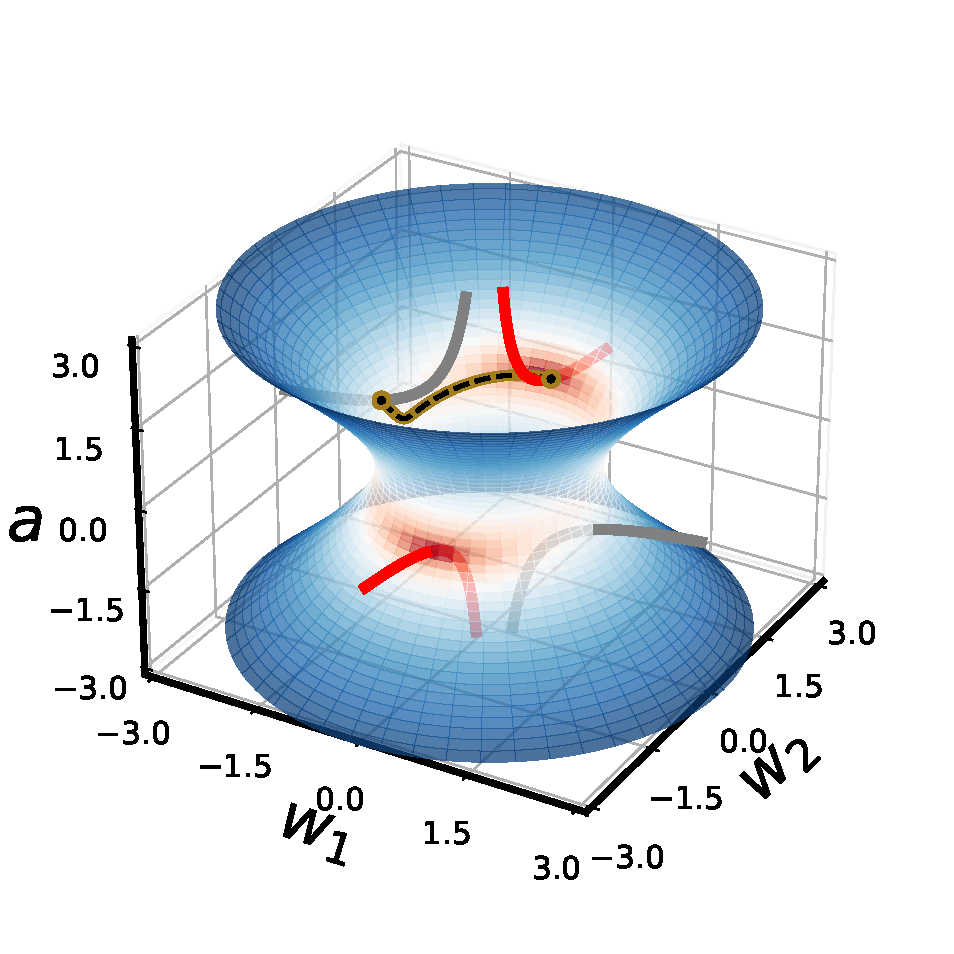
\includegraphics[width=\linewidth]{fig/single-neuron/negative.pdf}
        \caption{$\delta = -2$}
    \end{subfigure}
    \begin{subfigure}{0.325\linewidth}
        \centering
        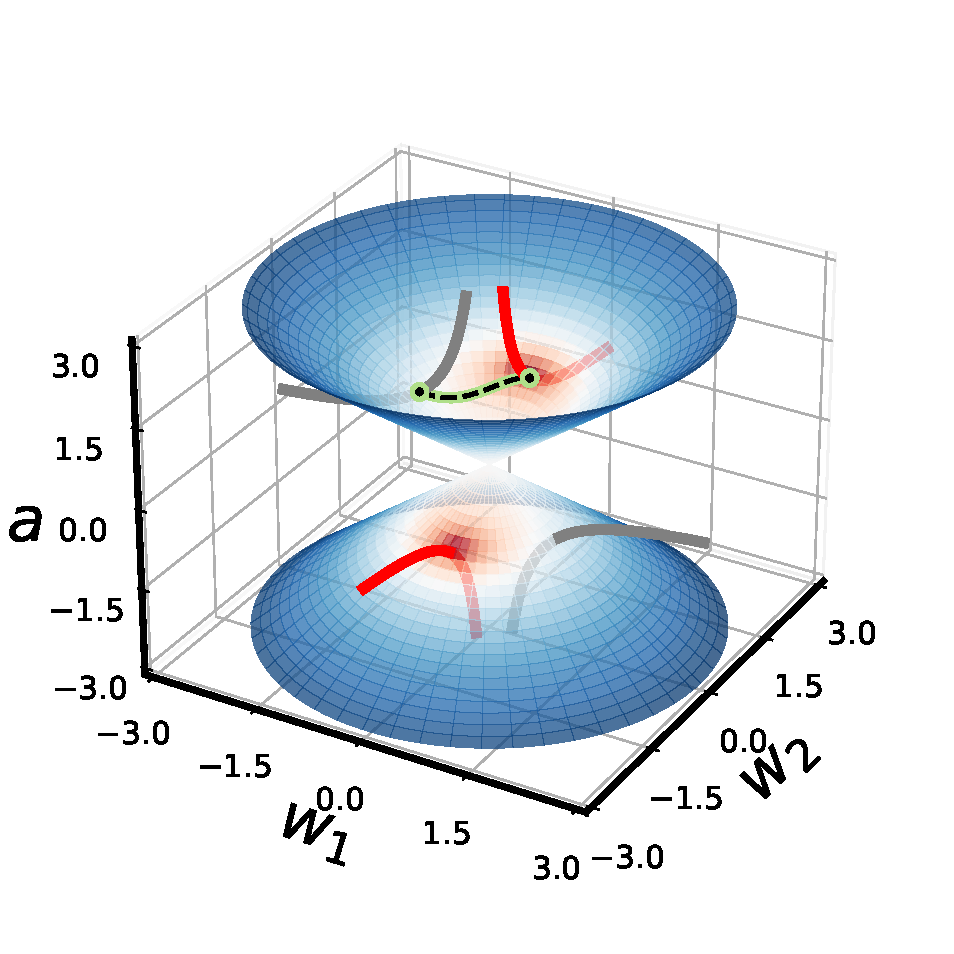
\includegraphics[width=\linewidth]{fig/single-neuron/zero.pdf}
        \caption{$\delta = 0$}
    \end{subfigure}
    \begin{subfigure}{0.325\linewidth}
        \centering
        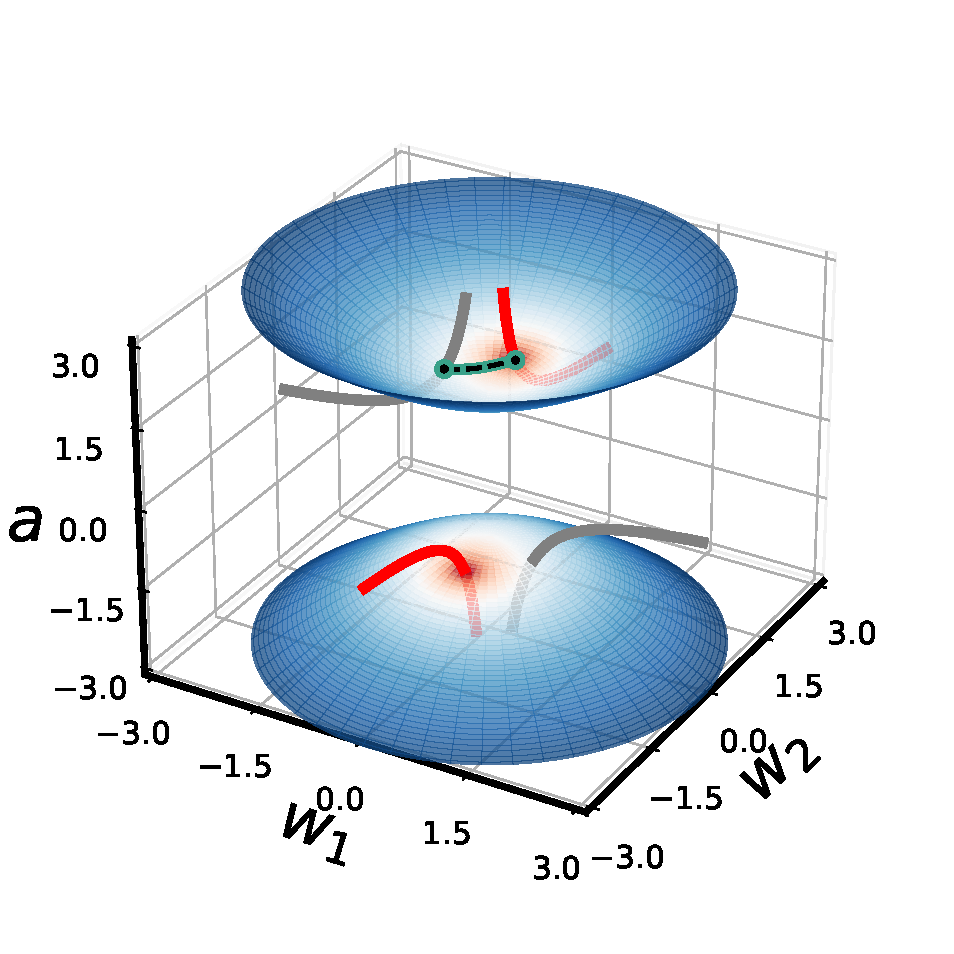
\includegraphics[width=\linewidth]{fig/single-neuron/positive.pdf}
        \caption{$\delta = 2$}
    \end{subfigure}
    \caption{\textbf{Balance determines geometry of trajectory.}
    %
    The quantity $\delta = \eta_wa^2 - \eta_a\|w\|^2$ is conserved through gradient flow, which constrains the trajectory to: (a) a one-sheeted hyperboloid for downstream initializations, (b) a double cone for balanced initializations, and (c) a two-sheeted hyperboloid for upstream initializations.
    %
    Gradient flow dynamics for three different initializations $a_0, w_0$ with the same product $\beta_0 = a_0w_0$ are shown.
    %
    The minima manifold is shown in red and the manifold of equivalent $\beta_0$ initializations in gray.
    %
    The surface is colored according to training loss, with blue representing higher loss and red representing lower loss.
    }
    \vspace{-8pt}
    \label{fig:single-neuron}
\end{wrapfigure}
\vspace{-10pt}
\section{A Minimal Model of Lazy and Rich Learning with Exact Solutions}
\label{sec:single-neuron}
\vspace{-5pt}



Here we explore an illustrative setting simple enough to admit exact gradient flow dynamics, yet complex enough to showcase lazy and rich learning regimes.
%
We study a two-layer linear network with a single hidden neuron defined by the map $f(x;\theta) = a w^\intercal x$ where $a \in \mathbb{R}$, $w \in \mathbb{R}^d$ are the parameters.
%
We examine how the parameter initializations $a_0, w_0$ and the layer-wise learning rates $\eta_{a}, \eta_{w}$ influence the training trajectory in parameter space, function space (defined by the product $\beta = aw$), and the evolution of the the NTK matrix,
%
\begin{equation}
    \label{eq:single-neuron-NTK-matrix}
    K = X \left(\eta_wa^2 \mathbf{I}_d + \eta_aww^\intercal\right)X^\intercal.
\end{equation}
%
Except for a measure zero set of initializations which converge to saddle points\footnote{The set of saddle points $\{(a,w)\}$ is the $d-1$ dimensional subspace satisfying $a = 0$ and $w^\intercal X^\intercal y = 0$.}, all gradient flow trajectories will converge to a global minimum, determined by the normal equations $X^\intercal X aw = X^\intercal y$.
%
However, even when $X^\intercal X$ is invertible such that the global minimum $\beta_*$ is unique, the rescaling symmetry between $a$ and $w$ results in a manifold of minima in parameter space.
%
The minima manifold is a one-dimensional hyperbola where $w \propto \beta_*$ and has two distinct branches for positive and negative $a$.
%
The symmetry also imposes a constraint on the network's trajectory, maintaining the difference $\delta = \eta_wa^2 - \eta_a\|w\|^2 \in \mathbb{R}$ throughout training (see \cref{app:single-neuron-conserved} for details).
%
This confines the parameter dynamics to the surface of a hyperboloid where the magnitude and sign of the conserved quantity determines the geometry, as shown in \cref{fig:single-neuron}.
%
An upstream initialization occurs when $\delta > 0$, a balanced initialization when $\delta = 0$, and a downstream initialization when $\delta < 0$.

\textbf{Deriving exact solutions in parameter space.}
%
We initially assume\footnote{We relax this assumption when considering the dynamics of $\beta$ in function space and their implicit bias.} whitened input $X^\intercal X = \mathbf{I}_d$ such that the ordinary least squares solution is $\beta_* = X^\intercal y$, and the gradient flow dynamics simplify to
$\dot{a} = \eta_a \left(w^\intercal \beta_* - a \|w\|^2\right)$, $\dot{w} = \eta_w \left(a\beta_* - a^2  w\right)$.
%
Notice that $w(t) \in \mathrm{span}(\{w_0, \beta_*\})$, and through training, $w$ aligns in direction to $\pm \beta_*$ depending on the basin of attraction\footnote{The basin is given by $\mathrm{sgn}(a_0)$ for $\delta \ge 0$ or $\mathrm{sgn}(w_0^\intercal \beta_* + \frac{a_0}{2} (\delta + \sqrt{\delta^2 + 4 \|\beta_*\|^2}))$ for $\delta < 0$. See \ref{app:single-neuron-basins}.} the parameters are initialized in.
%
Therefore, we can monitor the dynamics by tracking the hyperbolic geometry between $a$ and $\|w(t)\|$ and the spherical angle between $w(t)$ and $\beta_*$. 
%
We study the variables $\mu = a \|w\|$, an invariant under the rescale symmetry, and $\phi = \frac{w^\intercal \beta_*}{\|w\|\|\beta_*\|}$, the cosine of the spherical angle.
%
From these two scalar quantities $\mu(t), \phi(t)$ and the initialization $a_0, w_0$, we can determine the trajectory $a(t)$ and $w(t)$ in parameter space.
%
The dynamics for $\mu, \phi$ are given by the coupled nonlinear ODEs,
\begin{equation}
    \label{eq:single-neuron-transformed-dynamics}
    \dot{\mu} = \sqrt{\delta^2 + 4\eta_a\eta_w\mu^2}\left(\phi\|\beta_*\| - \mu\right),\qquad
    \dot{\phi} =  \frac{\eta_a\eta_w2\mu\|\beta_*\|}{\sqrt{\delta^2 + 4\eta_a\eta_w\mu^2} - \delta}\left(1 - \phi^2\right).
\end{equation}
Amazingly, this system can be solved exactly, as discussed in \cref{app:single-neuron-exact-solutions}, and shown in \cref{fig:single-neuron-exact-dynamics}.
%
Without delving into the specifics, we can develop an intuitive understanding of the solutions by examining the influence of the relative scale $\delta$.



\begin{wrapfigure}{R}{0.63\textwidth}
    \vspace{-14pt}
    \begin{subfigure}{0.325\linewidth}
        \centering
        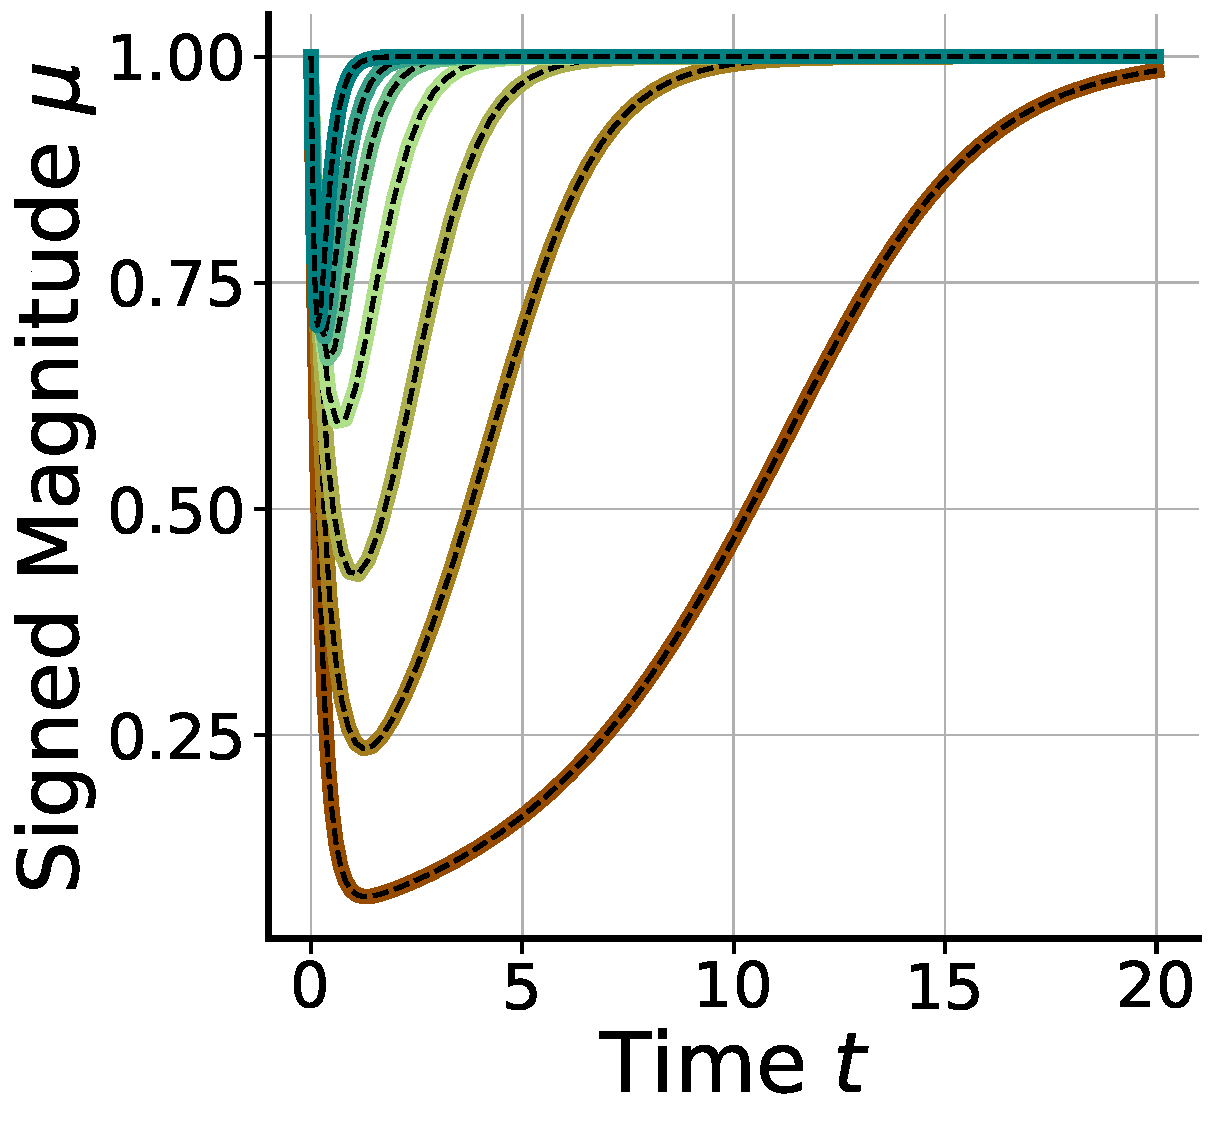
\includegraphics[width=\linewidth]{fig/single-neuron/mu.pdf}
        \caption{$\mu(t)$}
    \end{subfigure}
    \begin{subfigure}{0.325\linewidth}
        \centering
        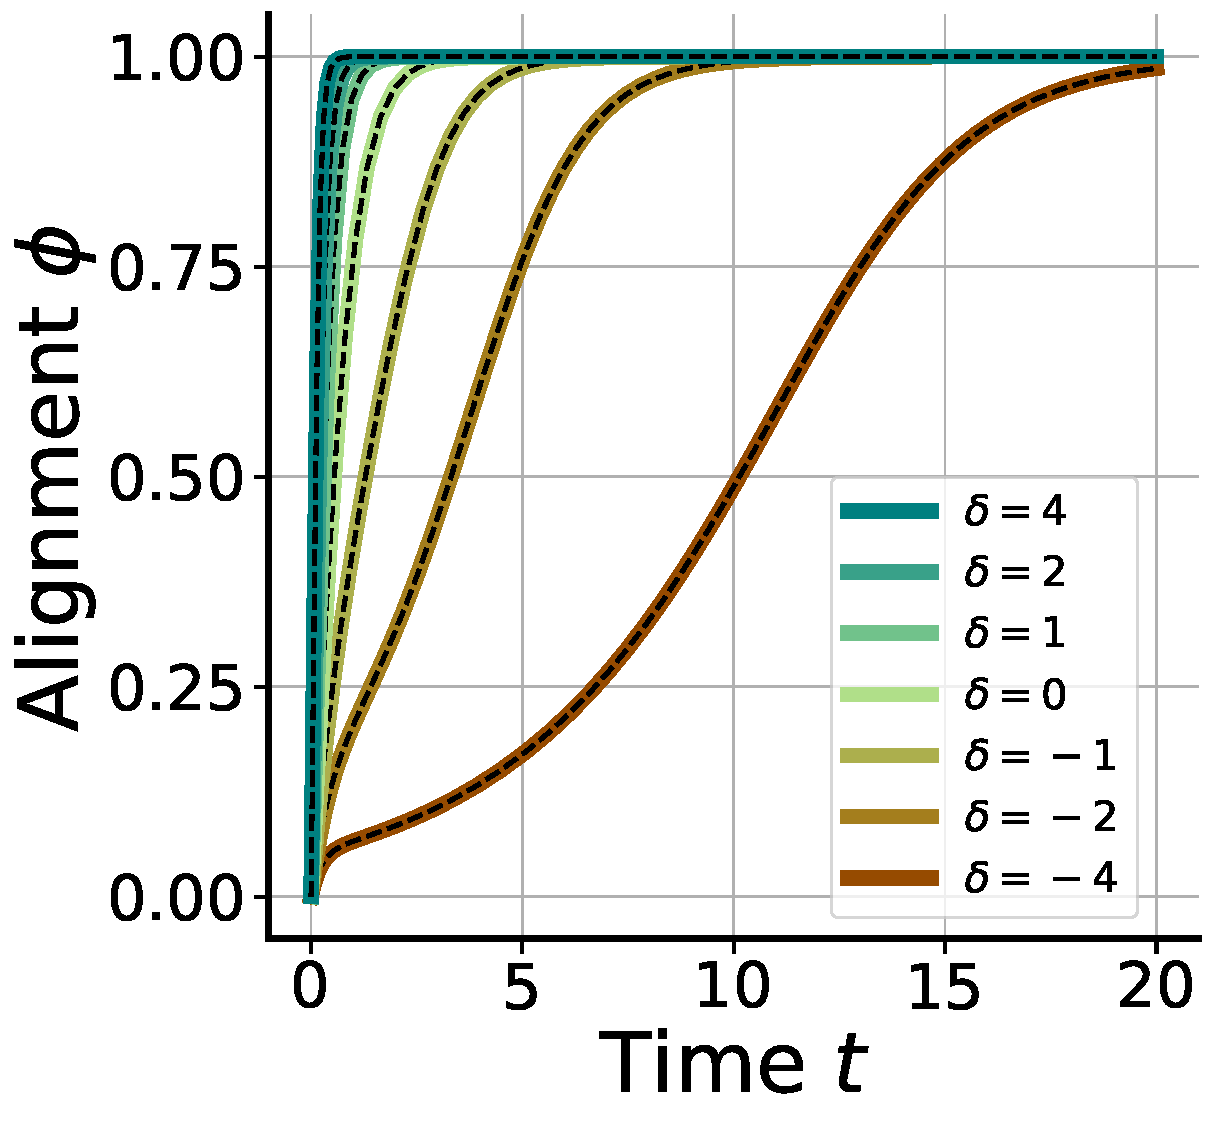
\includegraphics[width=\linewidth]{fig/single-neuron/phi.pdf}
        \caption{$\phi(t)$}
    \end{subfigure}
    \begin{subfigure}{0.325\linewidth}
        \centering
        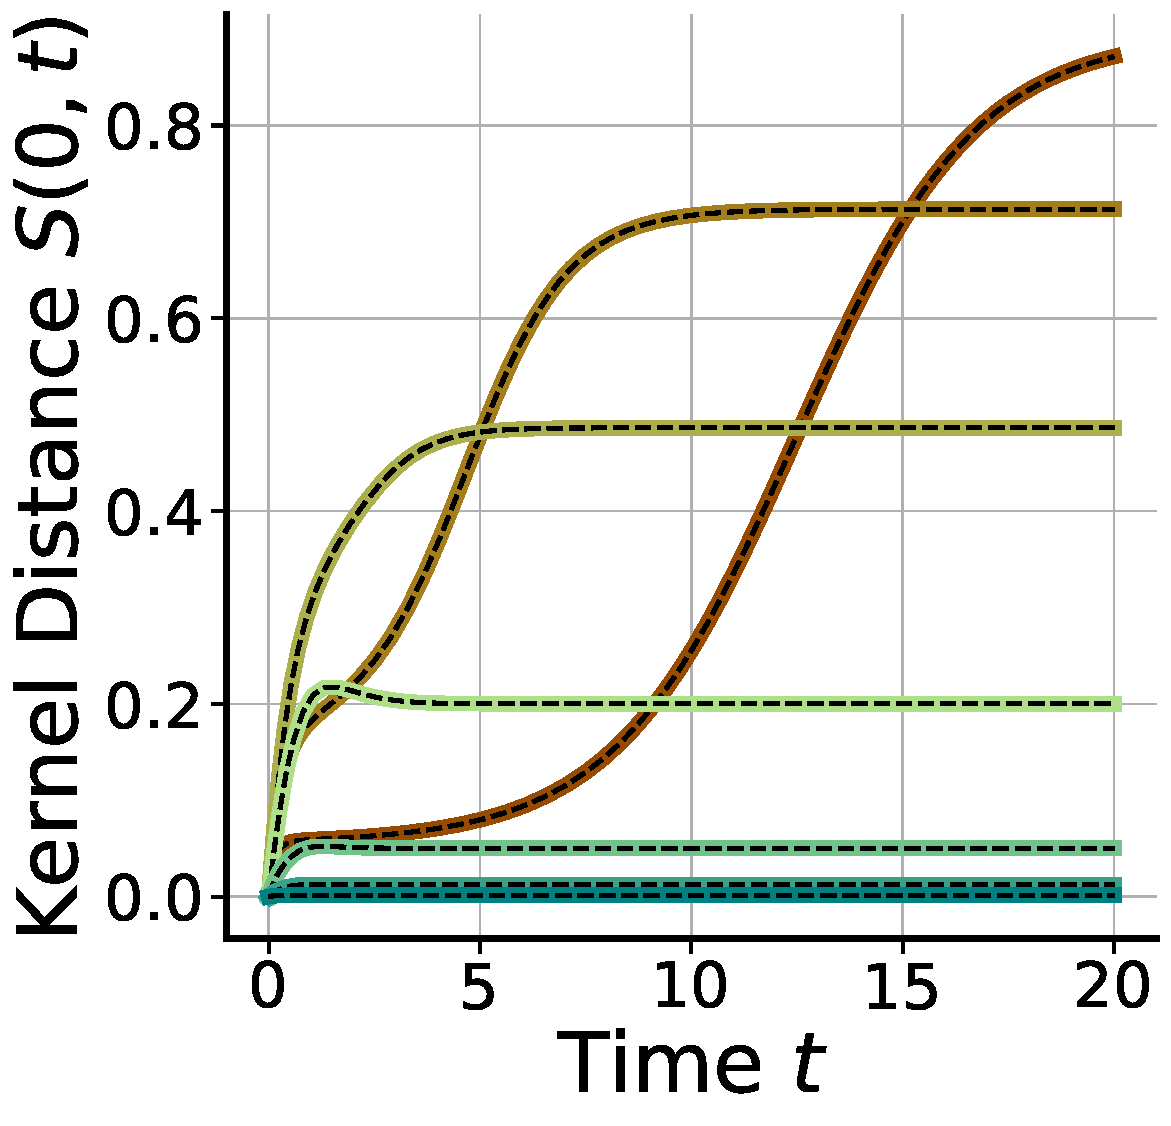
\includegraphics[width=\linewidth]{fig/single-neuron/kernel-distance.pdf}
        \caption{$S(0,t)$}
    \end{subfigure}
    \caption{
    \textbf{Exact solutions for the single hidden neuron model.}
    %
    Our theoretical predictions (black dashed lines) agree with gradient flow simulations (solid lines, color-coded based on $\delta$ values), shown here for three key metrics: $\mu$ (left), $\phi$ (middle), and $S(0,t)$ (right).
    %
    Each metric starts at the same value for all $\delta$, but varying $\delta$ has a pronounced effect on the metric's dynamics.
    %
    For upstream initializations ($\delta \gg 0$), $\mu$ changes only slightly, $\phi$ exponentially aligns, and $S$ remains near zero, indicative of the lazy regime.
    %
    For balanced initializations ($\delta = 0$), both $\mu$ and $\phi$ change significantly and $S$ quickly moves away from zero, indicative of the rich regime.
    %
    For downstream initializations ($\delta \ll 0$), $\mu$ quickly drops to zero, then $\mu$ and $\phi$ slowly climb back to one. 
    %
    Similarly, $S$ remains small before a sudden transition towards one, indicative of a delayed rich regime.
    %
     See \cref{app:single-neuron-exact-solutions} for further details.
    }
    \vspace{-18pt}
    \label{fig:single-neuron-exact-dynamics}
\end{wrapfigure}





\emph{\textbf{Upstream.}}
%
When $\delta \gg 0$, the updates for both $\mu$ and $\phi$ diverge, but $\phi$ updates much more rapidly.
%
We can decouple the dynamics of $\mu$ and $\phi$ by separation of their time scales and assume $\phi$ has reached its steady-state of $\pm 1$ before $\mu$ has updated.
%
Then, the dynamics of $\mu$ is linear and proceeds exponentially to $\pm \|\beta_*\|$.
%
This regime exhibits minimal kernel movement (see \cref{fig:single-neuron-exact-dynamics} (c)) because the kernel is dominated by the $\eta_wa^2\mathbf{I}_d$ term, whereas it is mainly $w$ that updates.

\emph{\textbf{Balanced.}}
%
When $\delta = 0$, $\mu$ follows a Bernoulli differential equation driven by a time-dependent signal $\phi \|\beta_*\|$, and $\phi$ follows a Riccati equation evolving from an initial value to $\pm 1$ depending on the basin of attraction.
%
For vanishing initialization $\|\beta_0\| \to 0$, the temporal dynamics of $\mu$ and $\phi$ decouple such that there are two phases of learning: 
an initial alignment phase where $\phi \to \pm 1$, followed by a fitting phase where $\mu \to \pm\|\beta_*\|$.
%
In the first phase, $w$ aligns to $\beta_*$ resulting in a rank-one update to the NTK, identical to the silent alignment effect described in \citet{atanasov2021neural}.
%
In the second phase, the dynamics of $\mu$ simplify to the Bernoulli equation studied in \citet{saxe2013exact} and the kernel evolves solely in overall scale.
% , where exact dynamics were also derived using a hyperbolic change of variables.

\emph{\textbf{Downstream.}}
%
When $\delta \ll 0$, the updates for $\mu$ diverge, while the updates for $\phi$ vanishes.
%
In this regime the dynamics proceed by an initial fast phase where $\mu$ converges exponentially to its steady state of $\phi\|\beta_*\|$.
%
Plugging this steady state into the dynamics of $\phi$ gives a Bernoulli differential equation $\dot{\phi} = \eta_a\eta_w\|\beta_*\|^2|\delta|^{-1}\phi(1 - \phi^2)$.
%
Due to the coefficient $|\delta|^{-1}$, the second alignment phase proceeds very slowly as $\phi$ approaches $\pm 1$, assuming $\phi, \mu \neq 0$, which is a saddle point.
%
In this regime, the dynamics proceed by an initial lazy fitting phase, followed by a rich alignment phase, where the delay is determined by the magnitude of $\delta$.



% Through this simple linear network, we can already determine how the initialization geometry determines when dynamics are in a lazy or rich regime.
% %
% Driving the distinctions is the value of $\delta$, which determines the geometry and topology of a hyperboloid constraining the learning trajectory.



\begin{wrapfigure}{R}{0.55\textwidth}
    \vspace{-15pt}
    \begin{subfigure}{0.49\linewidth}
        \centering
        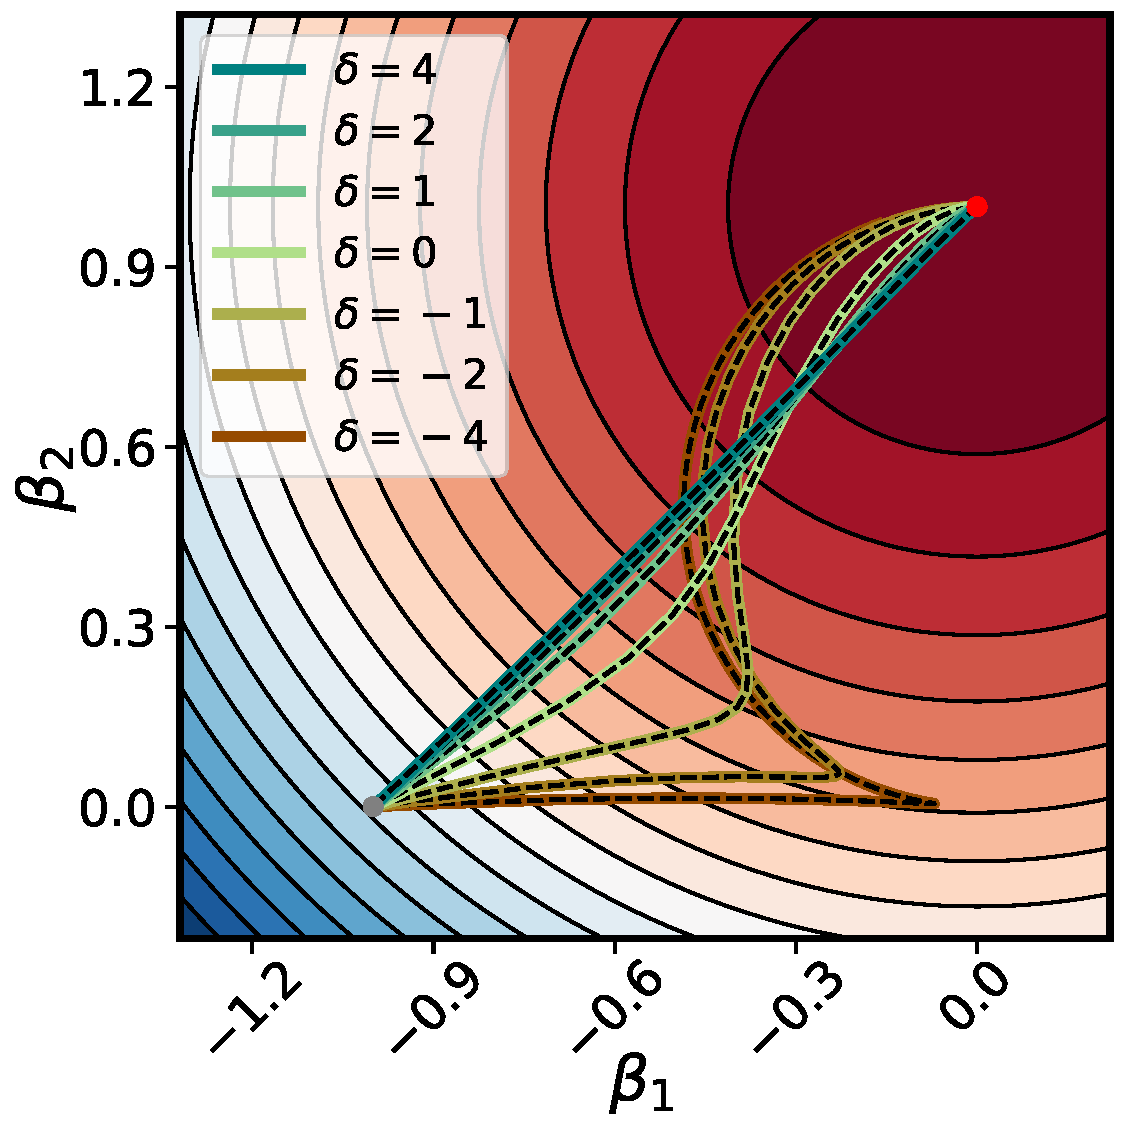
\includegraphics[width=\linewidth]{fig/single-neuron/function-space-whitened.pdf}
        \caption{Whitened $X^\intercal X$}
    \end{subfigure}
    \begin{subfigure}{0.49\linewidth}
        \centering
        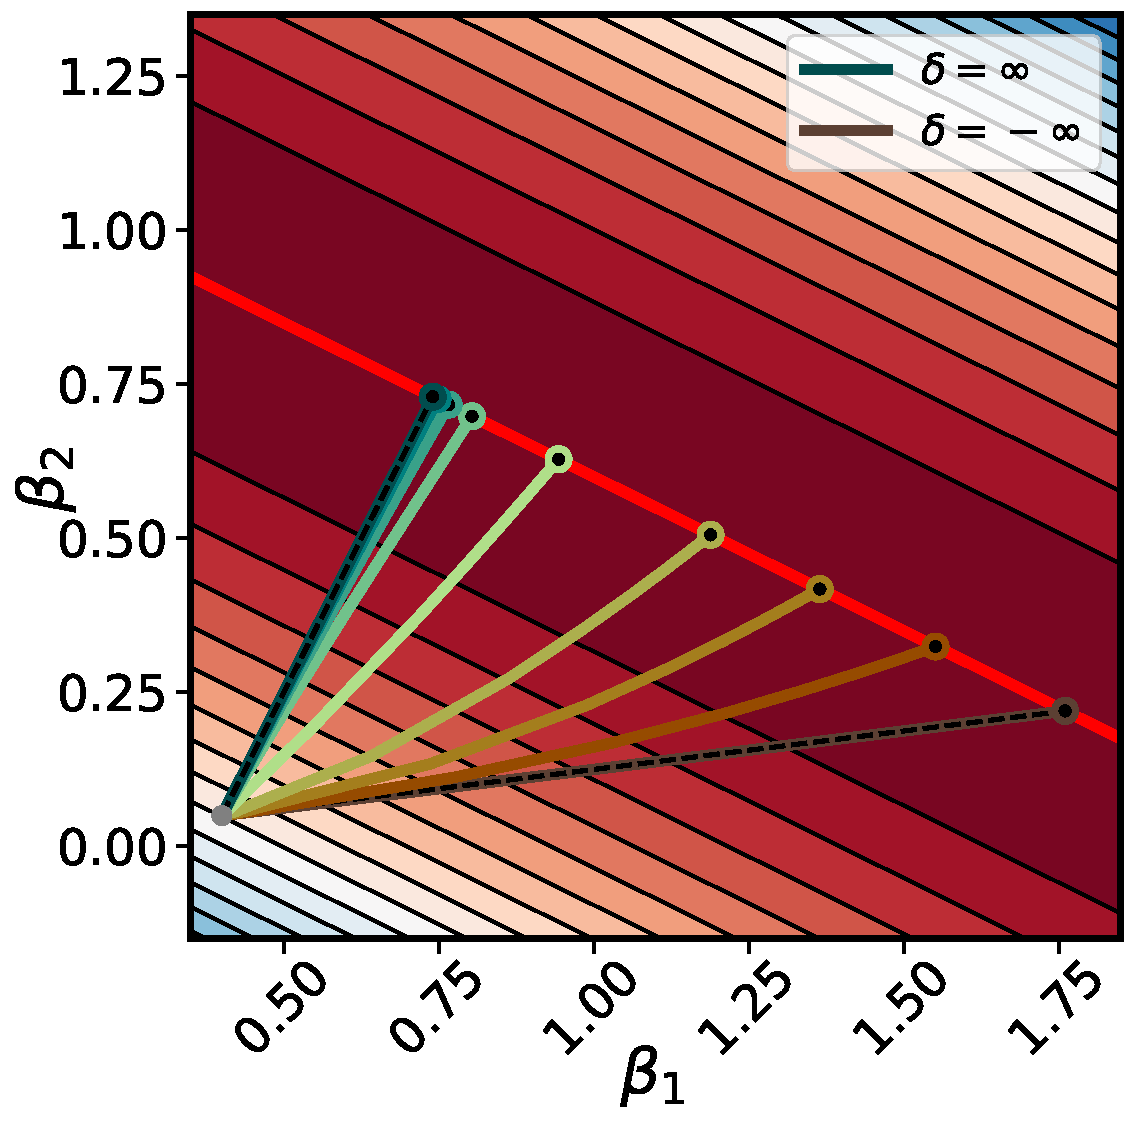
\includegraphics[width=\linewidth]{fig/single-neuron/function-space-low-rank.pdf}
        \caption{Low-Rank $X^\intercal X$}
    \end{subfigure}
    \caption{\textbf{Balance modulates $\beta$ dynamics and implicit bias.}
    Here we show the dynamics of $\beta = a w$ with different values of $\delta$, but the same initial $\beta_0$.
    %
    When $X^\intercal X$ is whitened (left), we can solve for the dynamics exactly using our expressions for $\mu, \phi$ (black dashed lines).
    %
    Upstream initializations follow the trajectory of gradient flow on $\beta$, downstream initializations first move in the direction of $\beta_0$ before sweeping around towards $\beta_*$, and balanced initializations take an intermediate trajectory between these two.
    %
    When $X^\intercal X$ is low-rank (right), then we can only predict the trajectories in the limit of $\delta = \pm \infty$.
    %
    If the interpolating manifold is one-dimensional, then we can solve for the solution in terms of $\delta$ exactly (black dots).
    %
    See \cref{app:single-neuron-inductive-bias} for details.
    }
    \vspace{-15pt}
    \label{fig:single-neuron-beta}
\end{wrapfigure}
%
\textbf{Identifying regimes of learning in function space.}
%
Here we take an alternative route towards understanding the influence of the relative scale by directly examining the dynamics in function space, an analysis strategy we will generalize to broader setups in~\cref{sec:wide-deep-linear,sec:nonlinear}.
%
The network's function is determined by the product $\beta = aw$ and governed by the ODE,
\begin{equation}
    \label{eq:beta_c_1_k_1}
    \dot{\beta} = -\underbrace{\left(\eta_w a^2\mathbf{I}_d + \eta_a w w^\intercal\right)}_{M} X^\intercal \rho,
\end{equation}
where $\rho = X \beta - y$ is the residual.
%
These dynamics can be interpreted as preconditioned gradient flow on the loss in function space where the preconditioning matrix $M$ depends on time through its dependence on $a^2$ and $ww^\intercal$.
%
Whenever $\|\beta\| \neq 0$, we can express $M$ directly in terms of $\beta$ and $\delta$ as
\begin{equation}
    \label{eq:M_c=1}
    M = \frac{\kappa + \delta}{2}\mathbf{I}_d + \frac{\kappa - \delta}{2}\frac{\beta\beta^\intercal}{\|\beta\|^2},
\end{equation}
where $\kappa = \sqrt{\delta^2 + 4\eta_a\eta_w\|\beta\|^2}$ (see \cref{app:single-neuron-beta} for a derivation).
%
This establishes a \emph{self-consistent} equation for the dynamics of $\beta$ regulated by $\delta$.
%
Additionally, notice that $M$ characterizes the NTK matrix \cref{eq:single-neuron-NTK-matrix}. 
%
Thus, understanding the evolution of $M$ along the trajectory $\beta_0$ to $\beta_*$ offers a method to discern between lazy and rich learning.
%
\emph{\textbf{Upstream.}} When $\delta \gg 0$, $M \approx \delta \mathbf{I}_d$, and the dynamics of $\beta$ converge to the trajectory of linear regression trained by gradient flow.
%
Along this trajectory the NTK matrix remains constant, confirming the dynamics are lazy.
%
\emph{\textbf{Balanced.}} When $\delta = 0$, $M = \sqrt{\eta_a\eta_w}\|\beta\|(\mathbf{I}_d + \tfrac{\beta\beta^\intercal}{\|\beta\|^2})$. %, where the second term is a projection matrix.
%
Here the dynamics balance between following the lazy trajectory and attempting to fit the task by only changing in norm.
%
As a result the NTK changes in both magnitude and direction through training, confirming the dynamics are rich.
%
\emph{\textbf{Downstream.}} When $\delta \ll 0$, $M \approx |\delta| \tfrac{\beta\beta^\intercal}{\|\beta\|^2}$, and $\beta$ follows a projected gradient descent trajectory, attempting to reach $\beta_*$ in the direction of $\beta_0$.
%
Along this trajectory the NTK matrix doesn't evolve.
%
However, if $\beta_0$ is not aligned to $\beta_*$, then at some point the dynamics of $\beta$ will slowly align.
%
In this second alignment phase the NTK matrix will change, confirming the dynamics are initially lazy followed by a delayed rich phase. 
% 
See \cref{app:single-neuron-kernel} for a derivation of the NTK dynamics $\dot{K}$.




\textbf{Determining the implicit bias via mirror flow.}
%
So far we have considered whitened or full rank $X^\intercal X$, ensuring the existence of a unique least squares solution $\beta_*$.
%
In this setting, $\delta$ influences the trajectory the model takes from $\beta_0$ to $\beta_*$, as shown in \cref{fig:single-neuron-beta} (a).
%
Now we consider low-rank $X^\intercal X$, such that there exist infinitely many interpolating solutions in function space.
%
By studying the structure of $M$, we can characterize how $\delta$ determines the interpolating solution the dynamics converge to.
%
Extending a time-warped mirror flow analysis strategy pioneered by \citet{azulay2021implicit} to allow $\delta < 0$ (see \cref{app:single-neuron-inductive-bias} for details), we prove the following theorem, which shows a tradeoff between reaching the minimum norm solution and preserving the direction of the initialization $\beta_0$.
\begin{theorem} [Extending Theorem 2 in \citet{azulay2021implicit}]
    \label{thrm:single-neuron-implicit-bias}
    For a single hidden neuron linear network, for any $\delta \in \mathbb{R}$, and initialization $\beta_0$ such that $\beta(t) \neq 0$ for all $t \ge 0$, if the gradient flow solution $\beta(\infty)$ satisfies $X \beta(\infty) = y$, then,
    \begin{equation}
        \beta(\infty) = \argmin_{\beta \in \mathbb{R}^d} \Psi_\delta(\beta) - \psi_\delta \tfrac{\beta_0}{\|\beta_0\|}^\intercal \beta \quad \mathrm{s.t.} \quad X \beta = y
    \end{equation}
    where $\Psi_\delta(\beta) = \frac{1}{3}\left(\sqrt{\delta^2 + 4\|\beta\|^2} - 2\delta\right)\sqrt{\sqrt{\delta^2 + 4\|\beta\|^2} + \delta}$ and $\psi_\delta = \sqrt{\sqrt{\delta^2 + 4\|\beta_0\|^2} - \delta}$.
\end{theorem}
We observe that for vanishing initializations there is functionally no difference between the inductive bias of the upstream ($\delta \gg 0$) and balanced ($\delta = 0$) settings.
%
However, in the downstream setting ($\delta \ll 0$), it is the second term preserving the direction of the initialization that dominates the inductive bias.
%
This tradeoff in inductive bias as a function of $\delta$ is presented in \cref{fig:single-neuron-beta} (b), where if the null space of $X^\intercal X$ is one-dimensional, we can solve for $\beta(\infty)$ in closed form (see \cref{app:single-neuron-inductive-bias}).


% At first glance it does not seem that the inductive bias presented in this theorem would be very interpretable, but again by studying the limiting behavior as a function of $\delta$ an interesting story emerges.
% %
% When $\delta \to \infty$, $Q_{\delta,\beta_0}(\beta) \to \|\beta\|^2$ and as would be expected the inductive bias in the lazy regime is simply the minimum Euclidean norm.
% %
% When $\delta = 0$, $Q_{\delta,\beta_0}(\beta) = \|\beta\|^{\frac{3}{2}} - \frac{3}{2} \frac{\beta^\intercal \beta_0}{\sqrt{\|\beta_0\|}}$.
%
% Now the inductive bias is given by a tradeoff between the minimum norm and preserving the direction of the initialization $\beta_0$.
% %
% For vanishing initialization there is functionally no difference between the inductive bias of the lazy or rich regimes in this setting.
% %
% However, for $\delta \to -\infty$, it is the second inner product term $z^\intercal \beta$ which dominates the inductive bias.
% %
% As a result if $\beta_0$ is not aligned to the minimum norm solution, then the inductive bias of the lazy-to-rich regime can be significantly different from either the lazy or rich.
%
% Additionally, if there exists an interpolating solution proportional to $\beta_0$, then the dynamics do not need to exit their initial lazy phase
%
% In fact, when the null space of $X^\intercal X$ is one-dimensional, the constrained optimization problem has an exact analytic solution, as presented in \cref{fig:single-neuron-beta}.

\vspace{-5pt}
\section{Wide and Deep Linear Networks}
\label{sec:wide-deep-linear}
\vspace{-5pt}

We now show how the analysis techniques used to study the influence of relative scale in the single-neuron setting can be applied to linear networks with multiple neurons, outputs, and layers.

\textbf{Wide linear networks.}
%
We consider the dynamics of a two-layer linear network with $h$ hidden neurons and $c$ outputs, $f(x;\theta) = A^\intercal W x$, where $W \in \mathbb{R}^{h \times d}$ and $A \in \mathbb{R}^{h \times c}$.
%
We assume $h \ge \min(d,c)$, such that this parameterization can represent all linear maps from $\mathbb{R}^d \to \mathbb{R}^c$.
%
The rescaling symmetry between $A$ and $W$ implies the $h \times h$ matrix $\Delta =  \eta_wA_0A_0^\intercal - \eta_aW_0W_0^\intercal$ is conserved throughout gradient flow \cite{du2018algorithmic}.
%
Drawing insights from our analysis of the single-neuron scenario ($h = c = 1$), 
%
we consider the dynamics of $\beta = W^\intercal A \in \mathbb{R}^{d \times c}$,
\begin{equation}
    \mathrm{vec}\left(\dot{\beta}\right) = -\underbrace{\left(\eta_wA^{\intercal}A \oplus \eta_aW^{\intercal}W\right)}_{M} \mathrm{vec}(X^\intercal X\beta - X^\intercal Y),
\end{equation}
where $\mathrm{vec}(\cdot)$ denotes the vectorization operator and $\oplus$ denotes the Kronecker sum\footnote{The Kronecker sum is defined for square matrices $C \in \mathbb{R}^{c \times c}$ and $D \in \mathbb{R}^{d \times d}$ as $C \oplus D = C \otimes \mathbf{I}_{d} + \mathbf{I}_{c} \otimes D$.}.
%
As in the single-neuron setting, we find that the dynamics of $\beta$ are preconditioned by a matrix $M$ that depends on quadratics of $A$ and $W$ and characterizes the NTK matrix $K = \left(\mathbf{I}_{c} \otimes X\right)M\left(\mathbf{I}_{c} \otimes X^\intercal\right)$.
%
We now show how $M$ can be expressed\footnote{When $h = c = 1$ we can recover \cref{eq:M_c=1} presented in the single-neuron setting directly from \cref{eq:Mi}.} in terms of the rank-1 matrices $\beta_k = w_ka_k^\intercal \in \mathbb{R}^{d \times c}$, which represent the contribution to $\beta$ of a single neuron with parameters $w_k$, $a_k$ and conserved quantity $\delta_k = \Delta_{kk}$.
% Add connection to projective and receptive fields - \citet{lehky1988network}
% In neuroscience, it has long been understood that comprehending the function of a neuron within a network requires knowledge of the weights constituting both its receptive and projective fields \citet{lehky1988network}.
%
% Here we see that rapid rich learning in linear networks can only occur when both the receptive and projective fields are learned and at similar speeds.
% 
% We see that lazy learning occurs when either just the receptive or projective field change to fit the task, while rich learning occurs when both learn by an appreciable amount.

\begin{theorem}
    \label{thrm:vec_beta}
    Whenever $\|\beta_k\|_F \neq 0$ for all $k \in [h]$, the matrix $M$ can be expressed as the sum $M = \sum_{k = 1}^h M_k$ over hidden neurons where $M_k$ is defined as,
    \begin{equation}
    \label{eq:Mi}
        M_k = \left(\frac{\sqrt{\delta_k^2 + 4\eta_a\eta_w\|\beta_k\|_F^2} + \delta_k}{2}\right)\frac{\beta_k^\intercal\beta_k}{\|\beta_k\|_F^2} \oplus \left(\frac{\sqrt{\delta_k^2 + 4\eta_a\eta_w\|\beta_k\|_F^2} - \delta_k}{2}\right)\frac{\beta_k\beta_k^\intercal}{\|\beta_k\|_F^2}.
    \end{equation}
\end{theorem}

%%%%% THE LIMITS OF M: %%%%%

% When $\delta = 0$, $M = \sum_{i = 1}^k \tfrac{\beta_k^\intercal \beta_k}{\|\beta_k\|_F} \oplus \sum_{i = 1}^k \tfrac{\beta_k \beta_k^\intercal}{\|\beta_k\|_F}$.

% As $\delta \to \infty$, $M \to \sum_{i = 1}^k |\delta_k|\tfrac{\beta_k^\intercal \beta_k}{\|\beta_k\|_F^2} \otimes \mathbf{I}_{d}$.

% As $\delta \to -\infty$, $M \to \mathbf{I}_{c} \otimes \sum_{i = 1}^k |\delta_k|\tfrac{\beta_k^\intercal \beta_k}{\|\beta_k\|_F^2}$.

By studying the dependence of $M$ on the conserved quantities $\delta_k$ and the dimensions $d$, $h$ and $c$, we can determine the influence of the relative scale on the learning regime.
%
When $\min (d,c) \le h < \max (d,c)$, and assuming independent initializations for all $\beta_k$, then networks which narrow from input to output ($d > c$) enter the lazy regime when all \(\delta_k \gg 0\), whereas networks which expand from input to output ($d < c$) do so when all \(\delta_k \ll 0\).
%
However, with opposite signs for $\delta_k$, and assuming all $\beta_k(0) \not\propto \beta_*$, these networks enter a \emph{delayed rich regime}.
%
As elaborated in \cref{app:wide-deep-linear-network-architectures},  this occurs because in these regimes a solution \(\beta_{*}\) does not exist within the space spanned by \(M\) at initialization.
%
When $h \ge \max (d,c)$ all networks enter the lazy regime when all $\delta_k \gg 0$ or all  $\delta_k \ll 0$.
%
Conversely, as all $\delta_k \to 0$, all networks  transition into the rich regime regardless of dimensions.
%
While \cref{thrm:vec_beta} offers valuable insight into the learning regimes in the limits of $\delta_k$, understanding the transition between regimes remains challenging. 
%
To achieve this, we aim to express $M$ in terms of $\beta$, rather than $\beta_k$, by introducing structure on the conserved quantities $\Delta$.


\begin{theorem}
    \label{thrm:vec_beta-isotropic}
    When $\Delta = \delta \mathbf{I}_h$ and $h = d$ if $\delta <0$ or $h = c$ if $\delta > 0$, then the matrix $M$ can be expressed as $M = \sqrt{\eta_a \eta_w\beta^{\intercal}\beta + \frac{\delta^2}{4}\mathbf{I}_c}   \otimes \mathbf{I}_d + \mathbf{I}_c \otimes \sqrt{\eta_a\eta_w \beta \beta^{\intercal} + \frac{\delta^2}{4}\mathbf{I}_d}$.
    % \begin{equation} \label{eq:M-isotropic}
    %     M = \left(\sqrt{\eta_a \eta_w\beta^{\intercal}\beta + \frac{\delta^2}{4}\mathbf{I}_c}   \otimes \mathbf{I}_d\right ) + \left(\mathbf{I}_c \otimes \sqrt{\eta_a\eta_w \beta \beta^{\intercal} + \frac{\delta^2}{4}\mathbf{I}_d}\right).
    % \end{equation}
\end{theorem}

From \cref{thrm:vec_beta-isotropic} the resulting dynamics of $\beta$ simplify to a self-consistent equation regulated by $\delta$,
\begin{equation}
    \dot{\beta} = -X^\intercal P \sqrt{\eta_a\eta_w \beta^\intercal\beta + \frac{\delta^2}{4} \mathbf{I}_c} - \sqrt{\eta_a\eta_w \beta\beta^\intercal + \frac{\delta^2}{4} \mathbf{I}_d}X^\intercal P,
\end{equation}
where $P = X\beta - Y$ is the residual.
% 
Under our isotropic assumption on the conserved quanitities $\Delta = \delta \mathbf{I}_h$, these dynamics are exact. Concurrent to our work, \citet{tu2024mixed} finds that $\beta$ \textit{approximately} follows these dynamics in the overparameterized setting $h \gg \max(d, c)$ under a Gaussian initialization $\mathcal{N}(0,\sigma^2)$ of the parameters where $\sigma^2 h$ is analogous to $\delta$.


Equipped with a self-consistent equation for the dynamics of $\beta$ we now aim to interpret these dynamics as a mirror flow with a $\delta$-dependent potential.
%
As presented in \cref{thrm:multi-neuron-singular}, the dynamics of the singular values of $\beta$ can be described as a mirror flow with a \emph{hyperbolic entropy} potential, which smoothly interpolates between an $\ell^1$ and $\ell^2$ penalty on the singular values for the rich ($\delta \to 0$) and lazy ($\delta \to \pm \infty$) regimes respectively.
%
This potential was first identified as the inductive bias for diagonal linear networks by \citet{woodworth2020kernel} and the same mirror flow on the singular values is derived from a different initialization choice in prior work by \citet{varre2024spectral}.
%
% See \cref{app:wide-deep-linear-network-mirror} for a further discussion.



\textbf{Deep linear networks}.
%
As presented in \cref{thm:deep-rich}, we generalize the inductive bias derived for rich two-layer linear networks by \citet{azulay2021implicit} to deep linear networks.
%
For a depth-$(L + 1)$ linear network, $f(x;\theta) = A^\intercal \prod_{l=1}^{L} W_l x$, where $\beta = \prod_{l=1}^{L} W_l^\intercal A$, we find that the inductive bias of the rich regime is $Q(\beta) = (\tfrac{L+1}{L+2})\|\beta\|^{\frac{L+2}{L+1}} - \|\beta_0\|^{-\frac{L}{L+1}}\beta_0^\intercal \beta$.
%
This inductive bias strikes a depth-dependent balance between attaining the minimum norm solution and preserving the initialization direction.

%
% Discuss the connection to describing the dynamics of $\beta$ as a preconditioned gradient flow in \citet{arora2018optimization} and other works discussing relationship between depth and nuclear norm in deep matrix factorization \cite{gunasekar2017implicit, arora2019implicit, li2020towards, ziyin2022exact}.
%
% Hierarchical learning in the lazy-to-rich regime.
% %
% Show what can happen when $d > k_1 > \dots > k_l > c$ in the lazy-to-rich regime such that there is a staircase effect where last layer learns, followed by second to last and so on.




\vspace{-10pt}
\section{Piecewise Linear Networks}
\label{sec:nonlinear}
\vspace{-5pt}

We now take a first step towards extending our analysis from linear networks to piecewise linear networks with activation functions of the form $\sigma(z) = \max(z, \gamma z)$. %, encompassing ReLU $\gamma = 0$ and Leaky ReLU $\gamma \in (0,1)$.
%
% \footnote{The subgradient $\sigma'(z) = 1$ if $z > 0$, $\sigma'(z) \in [\gamma, 1]$ if $z = 0$, and $\sigma'(z) = \gamma$ if $z < 0$.}
%
% These activation functions exhibit positive homogeneity, implying $\sigma(z) = \sigma'(z) z$ where $\sigma'(z)$ represents the subgradient, while also preserving a comparable rescaling symmetry to linear networks, resulting in a conserved quantity at each hidden neuron \cite{du2018algorithmic}.
%
The input-output map of a piecewise linear network with $L$ hidden layers and $h$ hidden neurons per layer is comprised of potentially $O(h^{dL})$ convex \emph{activation regions} \cite{raghu2017expressive}.
%
Each region is defined by a unique \emph{activation pattern} of the hidden neurons.
%
The input-output map is linear within each region and continuous at the boundary between regions. 
%
Collectively, the activation regions form a 2-colorable\footnote{To our knowledge, this property has not been recognized before. See \cref{app:nonlinear-surface} for a formal statement.} convex partition of input space, as shown in \cref{fig:xor-dynamics}.
%
We investigate how the relative scale influences the evolution of this partition and the linear maps within each region.



\textbf{Two-layer network.}
%
We consider the dynamics of a two-layer piecewise linear network without biases, $f(x;\theta) = a^\intercal \sigma(W x)$, where $W \in \mathbb{R}^{h \times d}$ and $a \in \mathbb{R}^h$.
%
% We permit $h > d$, which in the limit as $h \to \infty$, ensures the network is sufficiently expressive to represent any continuous function from $\mathbb{R}^d$ to $\mathbb{R}$ passing through the origin \cite{hornik1989multilayer}.
%
Following the approach in \cref{sec:wide-deep-linear}, we consider the contribution to the input-output map from a single hidden neuron $k \in [h]$ with parameters $w_k \in \mathbb{R}^d$, $a_k \in \mathbb{R}$ and conserved quantity $\delta_k = \eta_w a_k^2 - \eta_a\|w_k\|^2$ \cite{du2018algorithmic}.
%
However, unlike the linear setting, the neuron's contribution to $f(x_i;\theta)$ is regulated by whether the input $x_i$ is in the neuron's \emph{active halfspace}. %, $\{x \in \mathbb{R}^d : w_k^\intercal x > 0\}$.
%
Let $C \in \mathbb{R}^{h \times n}$ be the matrix with elements $c_{ki} = \sigma'(w_k^\intercal x_i)$, which determines the activation of the $k^{\mathrm{th}}$ neuron for the $i^{\mathrm{th}}$ data point. 
%
The dynamics of $\beta_k = a_kw_k$ are,
\begin{equation}
    \dot{\beta}_k = -\underbrace{\left(\eta_wa_k^2\mathbf{I}_d + \eta_aw_kw_k^\intercal\right)}_{M_k}\underbrace{\textstyle\sum_{i=1}^nc_{ki}x_i(f(x_i;\theta) - y_i)}_{\xi_k}.
\end{equation}
%
The matrix $M_k \in \mathbb{R}^{d \times d}$ is a preconditioning matrix on the dynamics, and when $\beta_k \neq 0$, it can be expressed in terms of $\beta_k$ and $\delta_k$.
%
Unlike the linear setting, $\xi_k \in \mathbb{R}^d$ driving the dynamics is not shared for all neurons because of its dependence on $c_{ki}$.
%
Additionally, the NTK matrix in this setting depends on $M_k$ and $C$, with elements $K_{ij} = \sum_{k = 1}^h c_{ki} x_i^\intercal M_k x_j c_{kj}$.
%
To examine the evolution of $K$, we consider a \emph{signed spherical coordinate} transformation separating the dynamics of $\beta_k$ into its directional $\hat{\beta}_k = \mathrm{sgn}(a_k)\tfrac{\beta_k}{\|\beta_k\|}$ and radial $\mu_k = \mathrm{sgn}(a_k)\|\beta_k\|$ components, such that $\beta_k = \mu_k \hat{\beta}_k$.
%
$\hat{\beta}_k$ determines the direction and orientation of the halfspace where the $k^{\mathrm{th}}$ neuron is active, while $\mu_k$ determines the slope of the contribution in this halfspace.
%
These coordinates evolve according to,
%
\begin{equation}
    \dot{\mu}_k = -\sqrt{\delta_k^2 + 4\eta_a\eta_w\mu_k^2}\hat{\beta}_k^\intercal \xi_k, \qquad
    \dot{\hat{\beta}}_k = -\frac{\sqrt{\delta_k^2 + 4\eta_a\eta_w\mu_k^2} + \delta_k}{2\mu_k} \left(\mathbf{I}_d - \hat{\beta}_k\hat{\beta}_k^\intercal\right)\xi_k.
\end{equation}
%
\emph{\textbf{Downstream.}}
%
When $\delta_k \ll 0 $, $M_k \approx |\delta_k|\hat{\beta}_k\hat{\beta}_k^\intercal$, and the dynamics are approximately $\partial_t\hat{\beta}_k = 0$ and $\partial_t\mu_k = -|\delta_k|\hat{\beta}_k^\intercal \xi_k$.
%
Irrespective of $\xi_k$, $\hat{\beta}_k(t) =  \hat{\beta}_k(0)$, which implies the overall partition map doesn't change (\cref{fig:xor-dynamics}, bottom), nor the activation patterns $C$, nor $M_k$.
%
Only $\mu_k$ changes to fit the data, while the NTK remains constant.
%
If the number of hidden neurons is insufficient to fit the data, there is a delayed rich alignment phase where the kernel will change, with $|\delta_k|$ determining the delay.


\emph{\textbf{Balanced.}}
When $\delta_k = 0$, $M_k = \sqrt{\eta_a\eta_w}|\mu_k|(\mathbf{I}_d + \hat{\beta}_k\hat{\beta}_k^\intercal)$, and the dynamics simplify to, $ \partial_t\hat{\beta}_k = -\sqrt{\eta_a\eta_w}\mathrm{sgn}(\mu_k)(\mathbf{I}_d - \hat{\beta}_k\hat{\beta}_k^\intercal)\xi_k$ and $\partial_t\mu_k = -2\sqrt{\eta_a\eta_w}|\mu_k|\hat{\beta}_k^\intercal \xi_k$.
%
Here both the direction and magnitude of $\beta_k$ evolve, resulting in changes to the activation regions, patterns $C$, and NTK $K$.
%
For vanishing initializations where $\|\beta_k(0)\| \to 0$ for all $k \in [h]$, we can decouple the dynamics into two distinct phases of training (\cref{fig:xor-dynamics}, top), analogous to the rich regime discussed in \cref{sec:single-neuron}.
%
\emph{Phase I: Partition alignment.} 
% 
At vanishing scale, the output $f(x;\theta_0) \approx 0$ for all input $x$, such that the vector driving the dynamics $\xi_k \approx -\sum_{i=1}^n c_{ki}x_iy_i$ is independent of the other hidden neurons. 
%
At the same time, the radial dynamics slow down relative to the directional dynamics, and the function's output will remain small as each neuron aligns to certain data-dependent fixed points, decoupled from the rest.
% 
Prior works have introduced structural constraints on the training data, such as orthogonally separable \cite{phuong2020inductive, wang2022early, min2023early}, pair-wise orthonormal \cite{boursier2022gradient}, linearly separable and symmetric \cite{lyu2021gradient} or small angle \cite{wang2024understanding}, to analytically determine the fixed points of this alignment phase.
%
\emph{Phase II: Data fitting.}
%
After enough time, the magnitudes of $\beta_k$ have grown such that we can no longer assume $f(x;\theta) \approx 0$ and thus the residual will depend on all $\beta_k$.
%
In this phase, the radial dynamics dominate the learning driving the network to fit the data.
%
However, it is possible for the directions to continue to change, and therefore some prior works have further decomposed this phase into multiple stages.

\begin{figure*}[t]
    \vspace{-15pt}
    \centering
    \begin{subfigure}{0.49\linewidth}
        \centering
        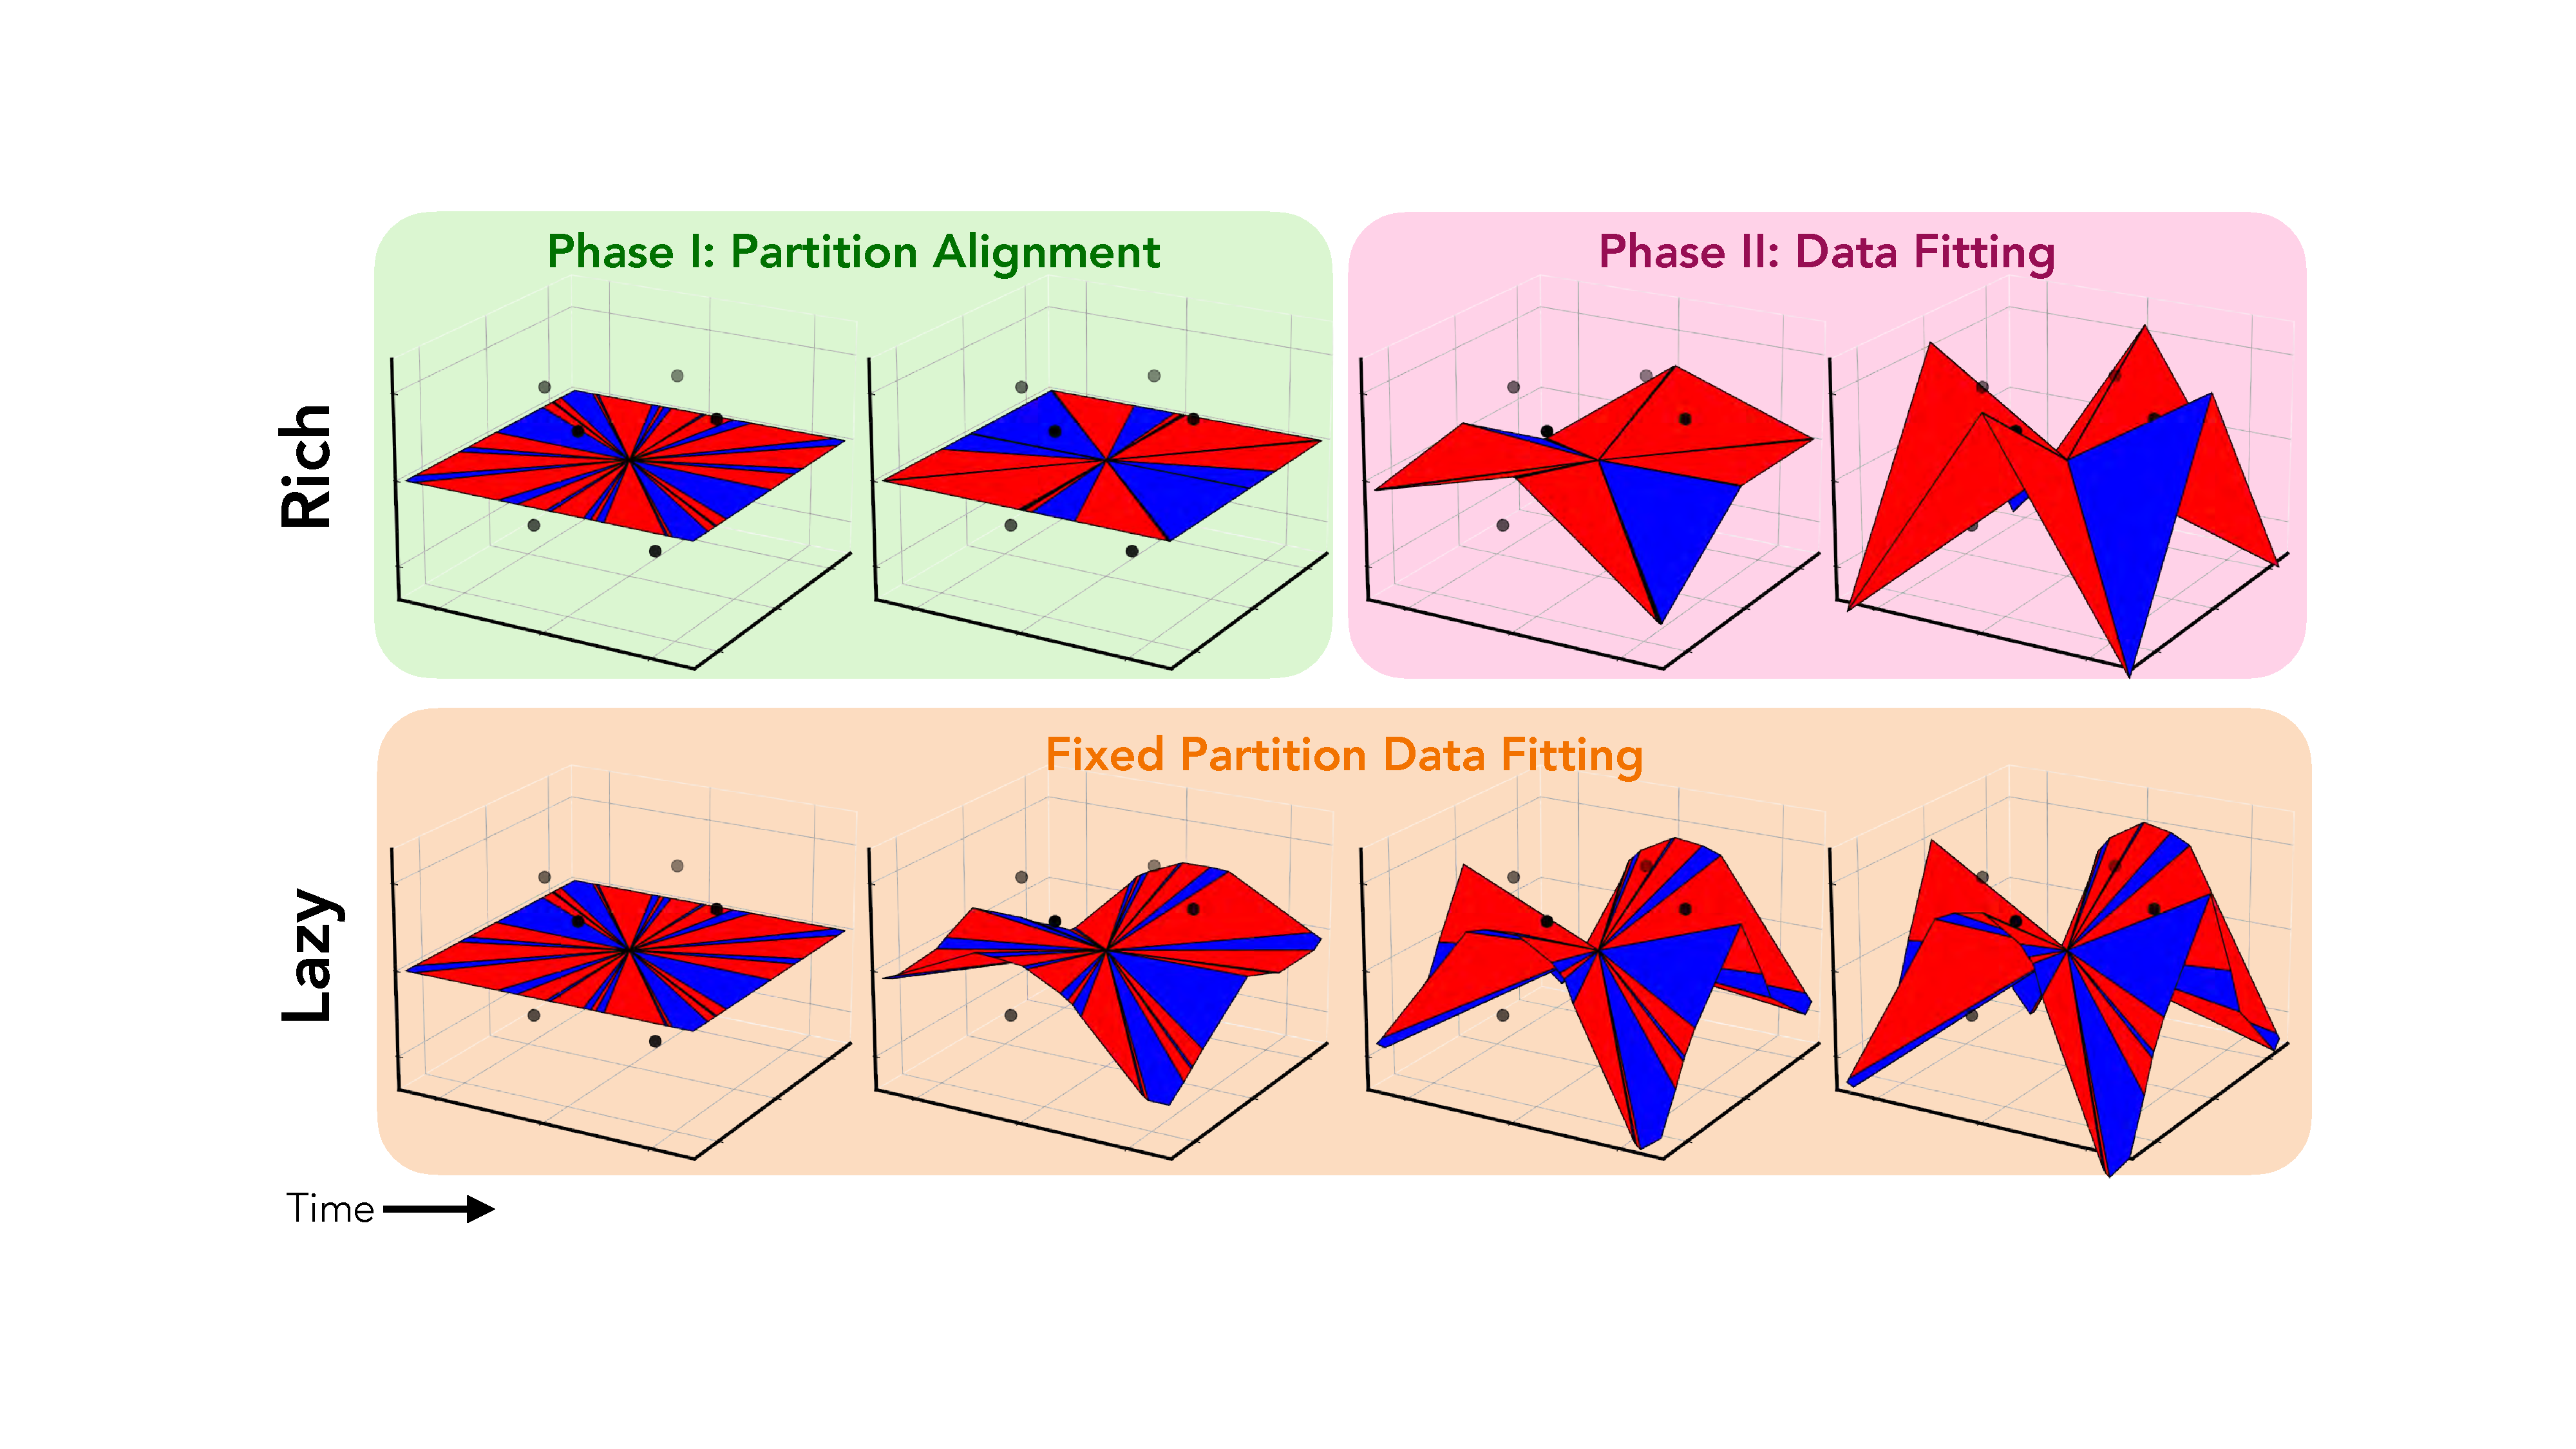
\includegraphics[width=\linewidth]{fig/ReLU-surface/fig5.pdf}
        \caption{Evolution of a ReLU network's input-output map}
    \end{subfigure}
    \begin{subfigure}{0.49\linewidth}
        \centering
        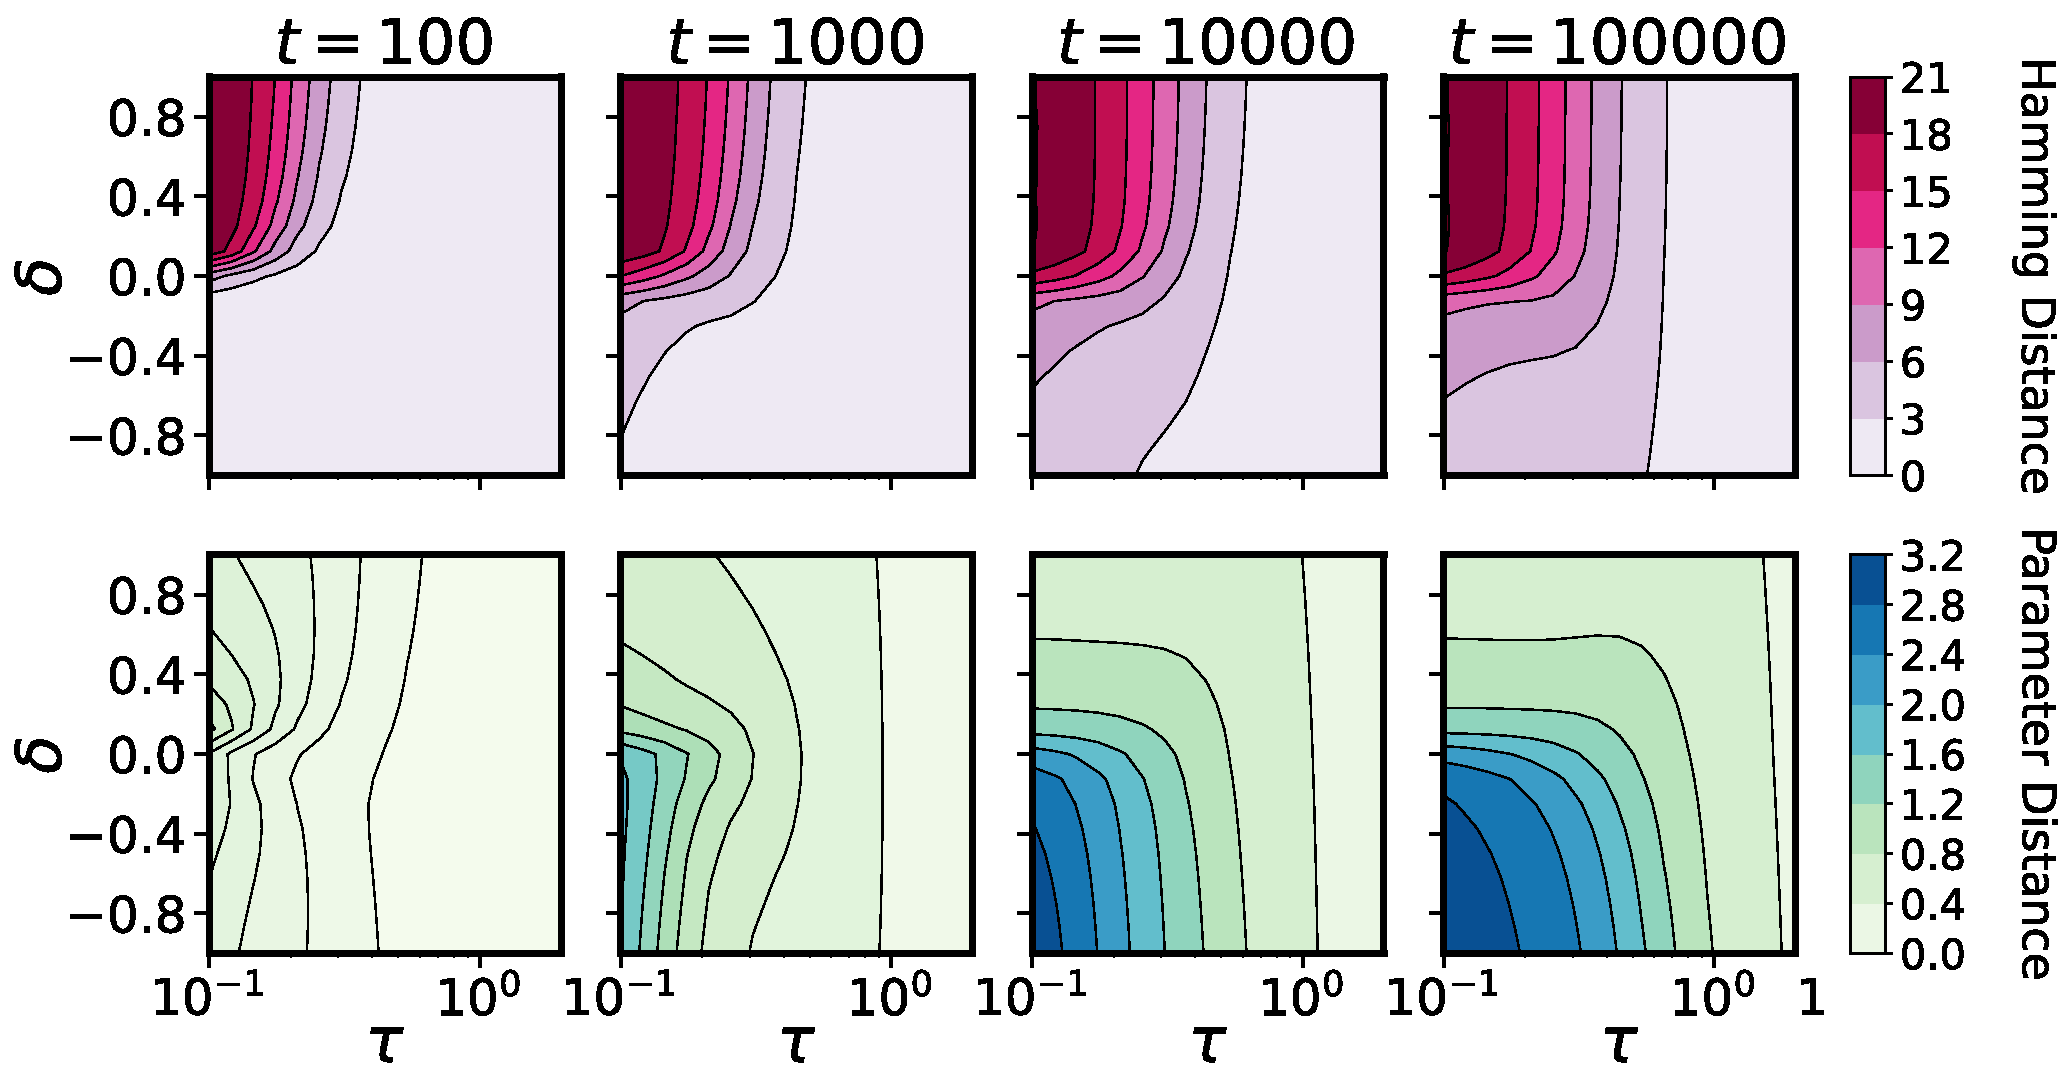
\includegraphics[width=\linewidth]{fig/two-layer/hamming-parameter.pdf}
        \caption{Hamming and parameter distance over $\tau$-$\delta$ sweep}
    \end{subfigure}
    \caption{
    \textbf{Rapid feature learning is caused by large activation changes with minimal parameter movement.}
    (a) We show the surface of a two-layer ReLU network trained on an XOR-like task, starting with a near-zero input-output map, $f(x;\theta_0)\approx0$. 
    %
    The surface consists of convex conic regions, each with a distinct activation pattern, colored by the parity of active neurons. 
    %
    A lazy initialization (\textit{bottom}) maintains a fixed activation partition throughout training, reweighting the hidden neurons to fit the data.
    %
    In contrast, a rich balanced or upstream initialization (\textit{top}) features an initial alignment phase where the partition map changes rapidly while the input-output map remains close to zero, followed by a data-fitting phase.
    %
    (b) We show the evolution of Hamming distance in activation patterns and parameter distance, relative to $t=0$, as a function of \textit{overall} and \textit{relative} scales (same experiments as in \cref{fig:two-layer-relu}(b)). \emph{Rapid feature learning} occurs from a small-$\tau$ upstream initialization that promotes faster learning in early layers, driving a large change in Hamming distance, but a small change in parameter space. In contrast, small-$\tau$ downstream initializations require large parameter movement to fit the data in the delayed rich regime.}
    \vspace{-20pt}
    \label{fig:xor-dynamics}
\end{figure*}

\emph{\textbf{Upstream.}}
%
When $\delta_k \gg 0$, $M_k \approx \delta_k \mathbf{I}_d$, and the dynamics are approximately $\partial_t\hat{\beta}_k = -\delta_k\mu_k^{-1}(\mathbf{I}_d - \hat{\beta}_k\hat{\beta}_k^\intercal)\xi_k$ and $\partial_t\mu_k = -\delta_k\hat{\beta}_k^\intercal \xi_k$.
%
Again, both the direction and magnitude of $\beta_k$ change.
%
However, unlike the balanced setting, in this setting $M_k$ is independent of $\beta_k$ and stays constant through training.
%
Yet, as $\beta_k$ change in direction, so can $C$, and thus the NTK.
%
This setting is unique, because it is rich due to a changing activation pattern, but the dynamics do not move far in parameter space.
%
Furthermore, unlike in the balanced scenario where scale adjusts the speed of radial dynamics, here it regulates the speed of directional dynamics, with vanishing initializations prompting an extremely fast alignment phase, as observed in \cref{fig:two-layer-relu} and in \cref{fig:xor-dynamics}.
%
% Mention how the directional dynamics scale proportionally with $\mu_k^{-1}$, while the radial dynamics are independent of $\mu_k$? Connect to supplementery figure for Fig. 1.  


\begin{figure*}[t]
    \begin{subfigure}{0.30\textwidth}
        \centering
        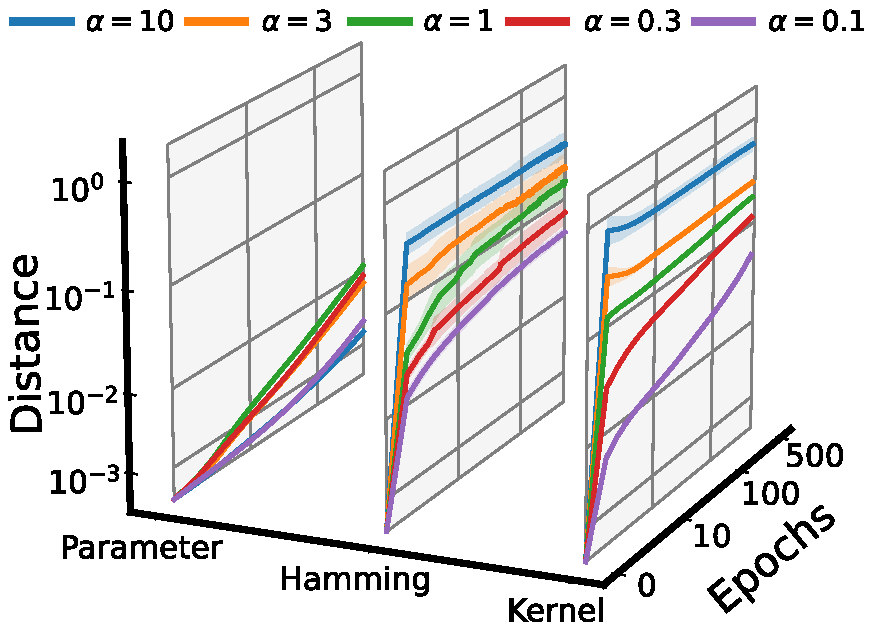
\includegraphics[width=\linewidth]{fig/deep-networks/kernel.pdf}
        \caption{Kernel Distance}
    \end{subfigure}
    \begin{subfigure}{0.22\textwidth}
        \centering
        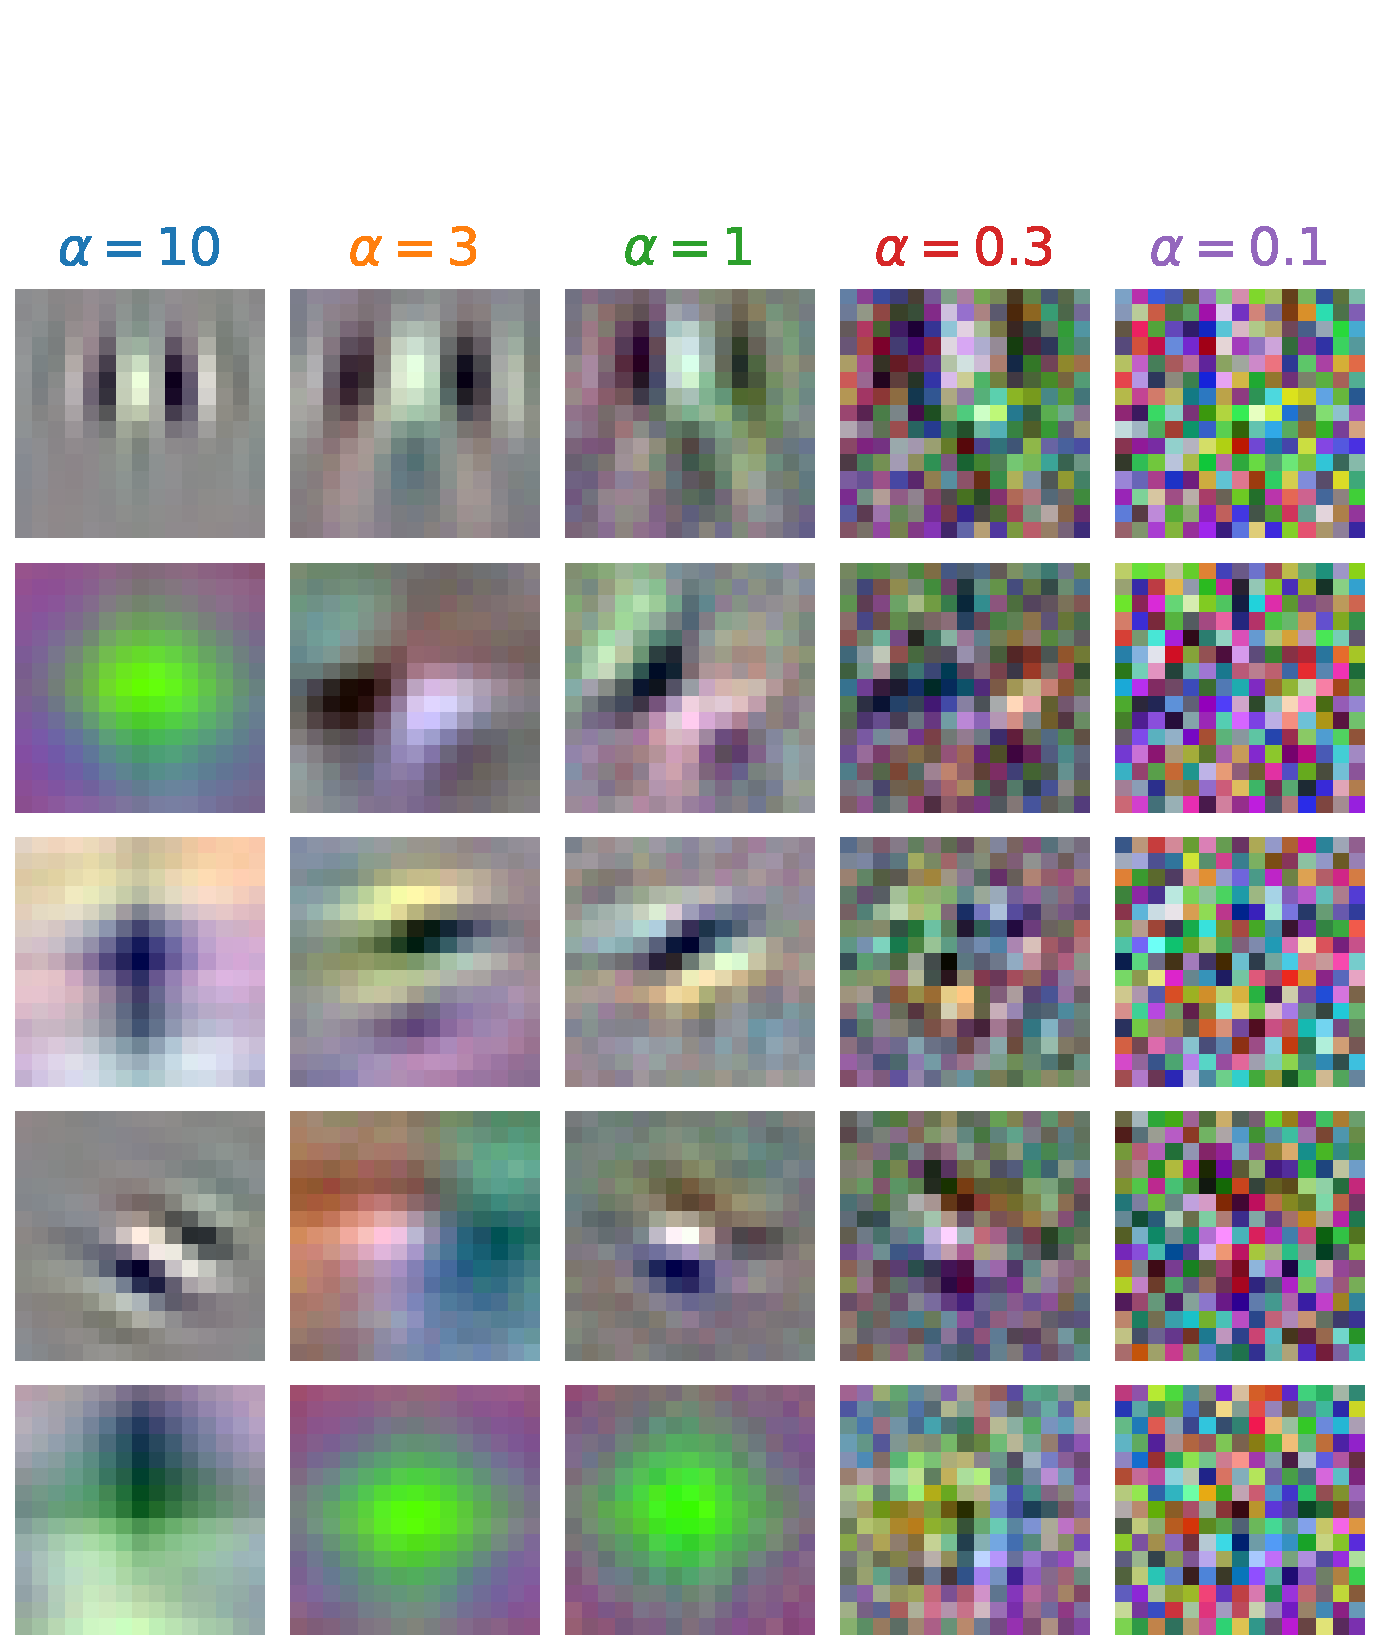
\includegraphics[width=\linewidth]{fig/deep-networks/gabors/gabors.pdf}
        \caption{Convolutional Filters}
    \end{subfigure}
    \begin{subfigure}{0.23\textwidth}
        \centering
        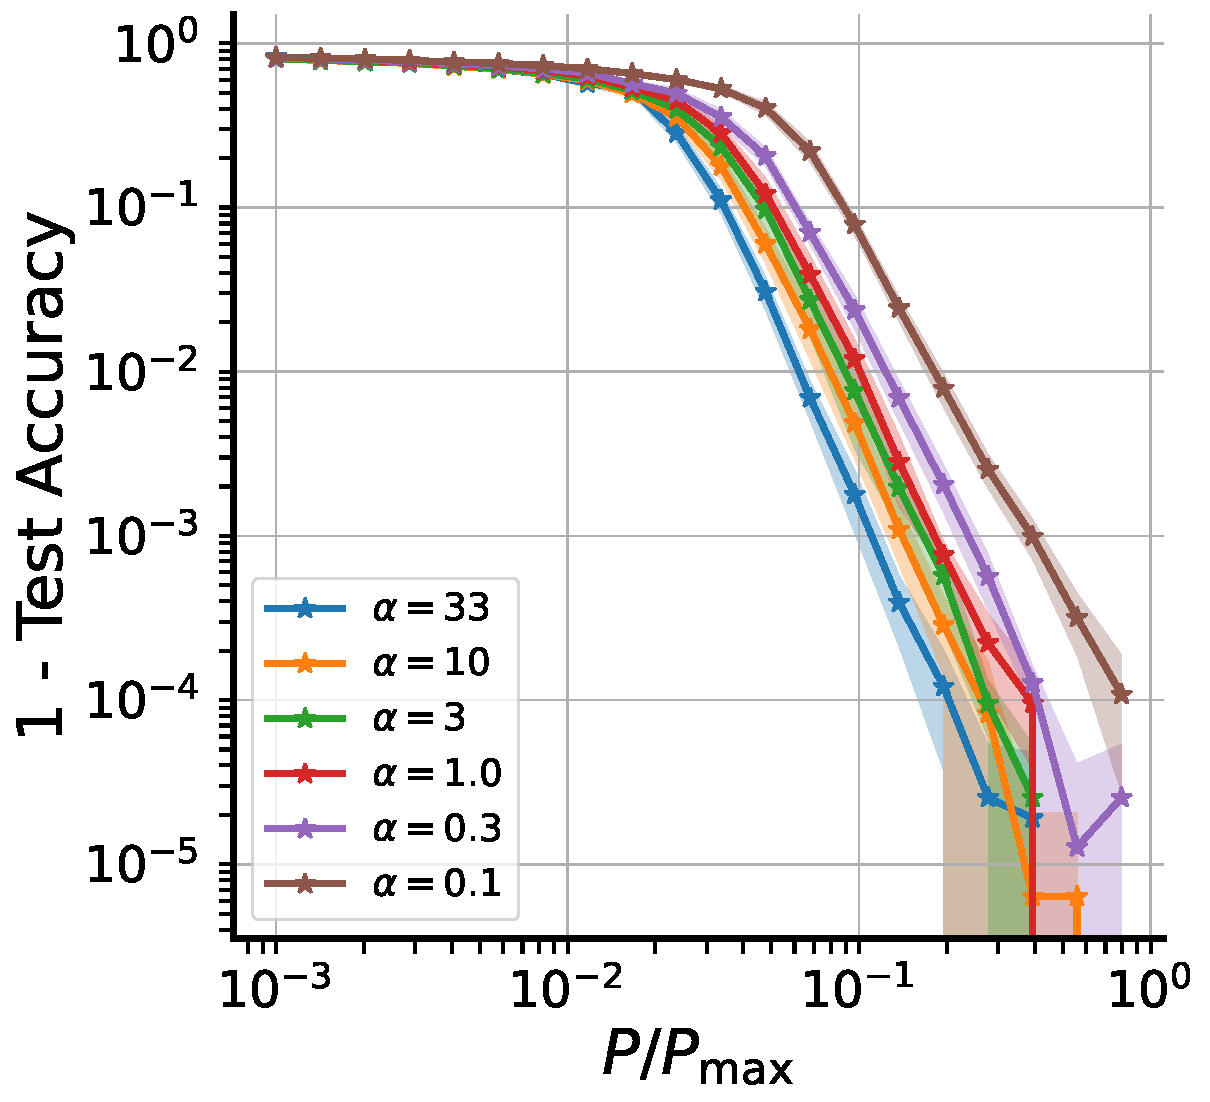
\includegraphics[width=\linewidth]{fig/deep-networks/rhm_v7.pdf}
        \caption{Random Hierarchy}
    \end{subfigure}
    \begin{subfigure}{0.23\textwidth}
        \centering
        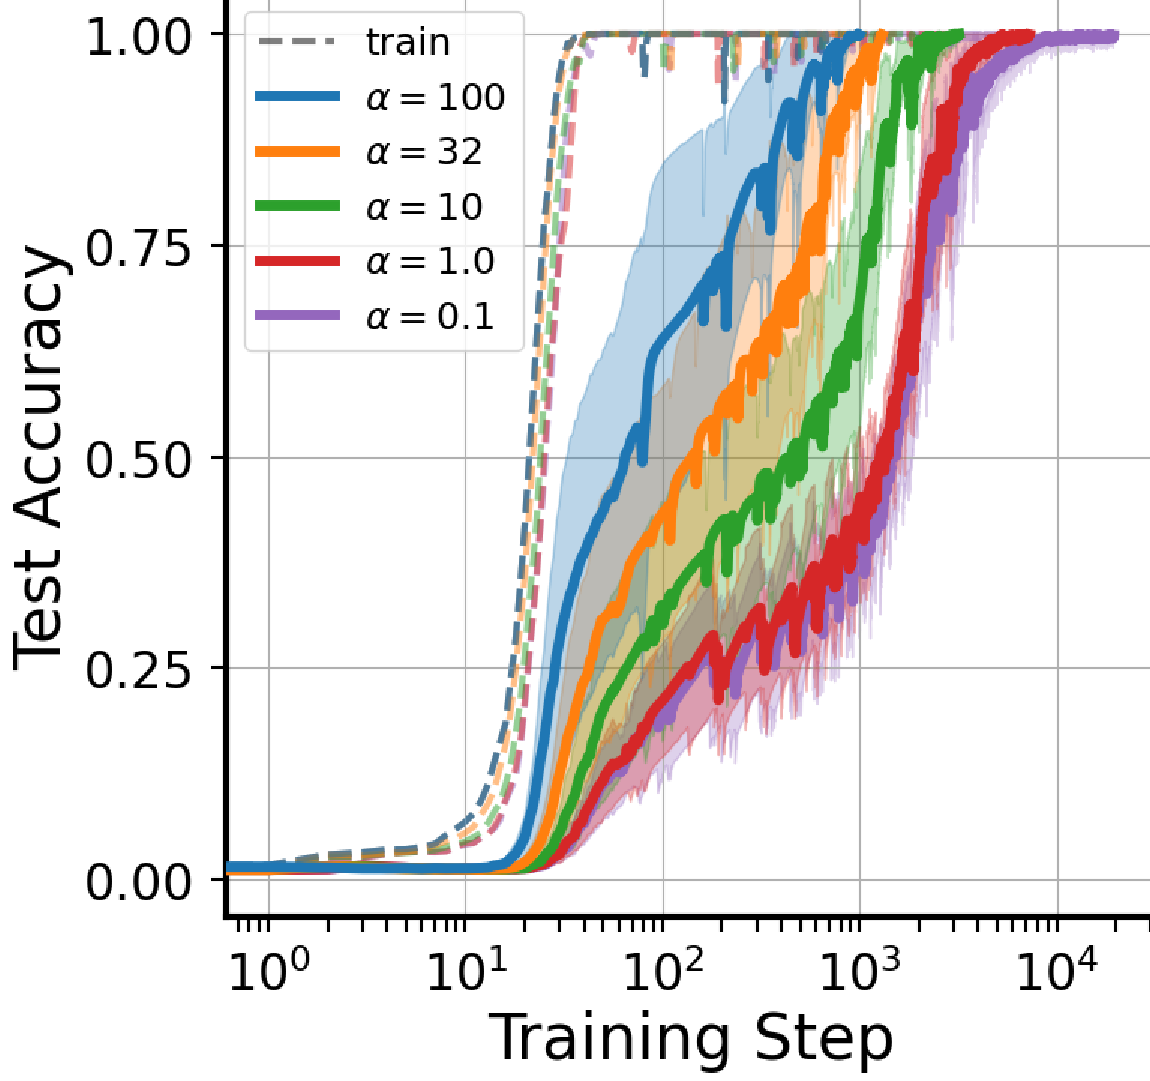
\includegraphics[width=\linewidth]{fig/deep-networks/grokking/grokking.pdf}
        \caption{Transformer Grokking}
    \end{subfigure}
    \caption{\textbf{Impact of upstream initializations in practice.}
    Here we provide evidence that an upstream initialization (a) drives feature learning through changing activation patterns, (b) promotes interpretability of early layers in CNNs, (c) reduces the sample complexity of learning hierarchical data, and (d) decreases the time to grokking in modular arithmetic.
    %
    In these experiments, we regulate the first layer's learning speed relative to the rest of the network by dividing its initialization by \(\alpha\). For models without normalization layers, we also scale the last layer's initialization by \(\alpha\) to preserve the input-output map. \(\alpha = 1\) represents standard parameterization, while \(\alpha \gg 1\) and \(\alpha \ll 1\) correspond to upstream and downstream initializations, respectively.
    %
    See \cref{app:fig-5} for details.}
    \label{fig:deep-network}
    \vspace{-18pt}
\end{figure*}

\textbf{Connections to infinite-width.} Our study of learning regimes in finite-width two-layer ReLU networks as a function of the overall and relative scale is consistent with existing infinite-width analysis of feature learning. For example, in \citet{luo2021phase} they consider a network $f(x) = \frac{1}{\alpha}\sum_{k = 1}^ha_k\sigma(w_k^\intercal x)$ with weights initialized as $a_k \sim \mathcal{N}(0, \beta_a^2)$ and $w_k \sim \mathcal{N}(0, \beta_W^2\mathbf{I}_d)$ as width $h\to\infty$. They obtain a phase diagram at infinite width capturing the dependence of learning regime on the overall function scale $\beta_a\beta_W/\alpha$ and the relative initialization scale $\beta_a/\beta_W$, each suitably normalized as a function of width. The resulting phase portrait is analogous to ours in \cref{fig:two-layer-relu} (b), where we use the conserved quantity $\delta$ rather than the relative scale $\beta_a/\beta_W$. Specifically, there is a lazy regime that includes the NTK parameterization, which is always achieved at large scale (as in the large-$\tau$ regions of \cref{fig:two-layer-relu} (b)), but is also achieved at small scale if the first layer variance is sufficiently larger than the second (as in the downstream initializations at small $\tau$ in \cref{fig:two-layer-relu} (b)). On the other side of the phase boundary is the infinite-width analog of rapid rich learning, where all neurons condense to a few directions. This is induced either at small function scale, or at larger scales if $\beta_a/\beta_W$ is sufficiently large, such that $W$ learns fast enough relative to $a$. The phase boundary, in turn, which exists only at infinite width, contains a range of parametrizations, including the mean-field parametrization.
%
More broadly, across width-dependent parametrizations, the random initialization of weights induces a distribution over per-neuron conserved quantities. 
%
While the distinction between the NTK and the mean-field parametrizations has been extensively studied, both lead to the same distribution of per-neuron conserved quantities, which is zero in expectation with a non-vanishing variance.
%
A more thorough study of what role the \textit{distribution} of per-neuron conserved quantities plays in feature learning at finite-widths is left to future work.


\textbf{Unbalanced initializations in practice.}
%
Our analysis shows that upstream initializations can drive rapid rich learning in nonlinear networks. 
% 
Further experiments in \cref{fig:deep-network} show that upstream initializations are relevant across various domains of deep learning:
%
(a) Standard initializations see significant NTK evolution early in training \cite{fort2020deep}. 
%
We show the movement is linked to changes in activation patterns rather than large parameter shifts. 
%
Adjusting the initialization variance of the first and last layers can amplify or diminish this movement.
%
(b) Filters in CNNs trained on image classification tasks often align with edge detectors \cite{krizhevsky2017imagenet}. 
%
We show that adjusting the learning speed of the first layer can enhance or degrade this alignment.
%
(c) Deep learning models are believed to avoid the curse of dimensionality and learn with limited data by exploiting hierarchical structures in real-world tasks.
%
Using the Random Hierarchy Model, introduced by \citet{petrini2023deep} as a framework for synthetic hierarchical tasks, we show that modifying the relative scale can decrease or increase the sample complexity of learning.
%
(d) Networks trained on simple modular arithmetic tasks will suddenly generalize long after memorizing their training data \cite{power2022grokking}. 
%
This behavior, termed grokking, is thought to result from a transition from lazy to rich learning \cite{kumar2023grokking, lyu2023dichotomy, rubin2024grokking} and believed to be important towards understanding emergent phenomena \cite{nanda2023progress}. 
%
We show that decreasing the variance of the embedding in a single-layer transformer ($<6\%$ of all parameters) significantly reduces the time to grokking.
%
% Overall, our experiments suggest that upstream initializations may play a crucial role in neural network behaviors.




\vspace{-10pt}
\section{Conclusion}
\label{sec:conclusion}
\vspace{-10pt}

In this work, we derived exact solutions to a minimal model that can transition between lazy and rich learning to precisely elucidate how unbalanced layer-specific initialization variances and learning rates determine the degree of feature learning.
%
We further extended our analysis to wide and deep linear networks and shallow piecewise linear networks.
%
We find through theory and empirics that unbalanced initializations, which promote faster learning at earlier layers, can actually accelerate rich learning.
%
\textbf{Limitations.}
%
The primary limitation lies in the difficulty to extend our theory to deeper nonlinear networks. 
%
In contrast to linear networks, where additional symmetries simplify dynamics, nonlinear networks require consideration of the activation pattern's impact on subsequent layers. 
%
One potential solution involves leveraging the path framework used in \citet{saxe2022neural}.
%
Another limitation is our omission of discretization and stochastic effects of SGD, which disrupt the conservation laws central to our study and introduce additional simplicity biases \cite{kunin2020neural, tanaka2021noether, chen2024stochastic, ziyin2024implicit}. 
%
\textbf{Future work.}
%
Our theory encourages further investigation into unbalanced initializations to optimize efficient feature learning. 
%
% In deep networks there are many ways to be unbalanced beyond upstream and downstream.
%
Understanding how the \emph{learning speed profile} across layers impacts feature learning, inductive biases, and generalization is an important direction for future work.

% FUTURE DIRECTIONS:
% 1. Extend exact single-neuron analysis to multiple neurons (potentially adding an assumption on their relative initialization)
% 2. Determining an exact characterization for the fixed points of the alignment phase of rich learning in piecewise linear network
% 3. Extending the nonlinear analysis to multiple layers.
% 4. Connecting our theory to more empirics of feature learning, such as the Average Gradient Outer Product mechanism for feature learning described in Misha Belkin's work?








%%%%%%%%%%%%%%%%%%%%%%%%%%%%%%%%%%%%%%%%%%%%%%%%%%%%%%%%%%%%
\clearpage
\begin{ack}
    We thank Francisco Acosta, Alex Atanasov, Yasaman Bahri, Abby Bertics, Blake Bordelon, Nan Cheng, Alex Infanger, Mason Kamb, Guillaume Lajoie, Nina Miolane, Cengiz Pehlevan, Ben Sorscher, Javan Tahir, Atsushi Yamamura for helpful discussions.
    %
    D.K. thanks the Open Philanthropy AI Fellowship for support.
    %
    S.G. thanks the James S. McDonnell and Simons Foundations, NTT Research, and an NSF CAREER Award for support.
    %
    This research was supported in part by grant NSF PHY-1748958 to the Kavli Institute for Theoretical Physics (KITP).
\end{ack}

\section*{Author Contributions}
This project originated from conversations between Daniel and Allan at the Kavli Institute for Theoretical Physics.
%
Daniel, Allan, and Feng are primarily responsible for the single neuron analysis in \cref{sec:single-neuron}.
%
Daniel, Clem, Allan, and Feng are primarily responsible for the wide and deep linear analysis in \cref{sec:wide-deep-linear}.
%
Daniel is primarily responsible for the nonlinear analysis in \cref{sec:nonlinear}.
%
Allan, Feng, and David are primarily responsible for the empirics in \cref{fig:two-layer-relu} and \cref{fig:deep-network}.
%
Daniel is primarily responsible for writing the main sections.
%
All authors contributed to the writing of the appendix and the polishing of the manuscript.

\bibliography{bibliography}
%%%%%%%%%%%%%%%%%%%%%%%%%%%%%%%%%%%%%%%%%%%%%%%%%%%%%%%%%%%%
\appendix



%%%%%%%%%%%%%%%%%%%%%%%%%%%%%%%%%%%%%%%%%%%%%%%%%%%%%%%%%%%%

% \newpage
% \section*{NeurIPS Paper Checklist}

% % %%% BEGIN INSTRUCTIONS %%%
% % The checklist is designed to encourage best practices for responsible machine learning research, addressing issues of reproducibility, transparency, research ethics, and societal impact. Do not remove the checklist: {\bf The papers not including the checklist will be desk rejected.} The checklist should follow the references and precede the (optional) supplemental material.  The checklist does NOT count towards the page
% % limit. 

% % Please read the checklist guidelines carefully for information on how to answer these questions. For each question in the checklist:
% % \begin{itemize}
% %     \item You should answer \answerYes{}, \answerNo{}, or \answerNA{}.
% %     \item \answerNA{} means either that the question is Not Applicable for that particular paper or the relevant information is Not Available.
% %     \item Please provide a short (1–2 sentence) justification right after your answer (even for NA). 
% %    % \item {\bf The papers not including the checklist will be desk rejected.}
% % \end{itemize}

% % {\bf The checklist answers are an integral part of your paper submission.} They are visible to the reviewers, area chairs, senior area chairs, and ethics reviewers. You will be asked to also include it (after eventual revisions) with the final version of your paper, and its final version will be published with the paper.

% % The reviewers of your paper will be asked to use the checklist as one of the factors in their evaluation. While "\answerYes{}" is generally preferable to "\answerNo{}", it is perfectly acceptable to answer "\answerNo{}" provided a proper justification is given (e.g., "error bars are not reported because it would be too computationally expensive" or "we were unable to find the license for the dataset we used"). In general, answering "\answerNo{}" or "\answerNA{}" is not grounds for rejection. While the questions are phrased in a binary way, we acknowledge that the true answer is often more nuanced, so please just use your best judgment and write a justification to elaborate. All supporting evidence can appear either in the main paper or the supplemental material, provided in appendix. If you answer \answerYes{} to a question, in the justification please point to the section(s) where related material for the question can be found.
 

% % %%% END INSTRUCTIONS %%%


% \begin{enumerate}

% \item {\bf Claims}
%     \item[] Question: Do the main claims made in the abstract and introduction accurately reflect the paper's contributions and scope?
%     \item[] Answer: \answerYes{}
%     \item[] Justification: The abstract clearly lays out the four main contributions sections of our paper (1) a novel minimal model of the transition between rich and lazy learning with exact solutions, (2) extension of this model to more complex linear networks, (3) application of this analysis to shallow nonlinear networks, (4) demonstration of the relevance of the unbalanced rich regime identified in practical deep learning settings. The claims made accurately match the theoretical and experimental results in the paper.
%     %
%     These four main contributions (also discussed in our contributions section in \cref{sec:introduction}) reflect \cref{sec:single-neuron}, \cref{sec:wide-deep-linear}, and \cref{sec:nonlinear}.
%     \item[] Guidelines:
%     \begin{itemize}
%         \item The answer NA means that the abstract and introduction do not include the claims made in the paper.
%         \item The abstract and/or introduction should clearly state the claims made, including the contributions made in the paper and important assumptions and limitations. A No or NA answer to this question will not be perceived well by the reviewers. 
%         \item The claims made should match theoretical and experimental results, and reflect how much the results can be expected to generalize to other settings. 
%         \item It is fine to include aspirational goals as motivation as long as it is clear that these goals are not attained by the paper. 
%     \end{itemize}

% \item {\bf Limitations}
%     \item[] Question: Does the paper discuss the limitations of the work performed by the authors?
%     \item[] Answer: \answerYes{} % Replace by \answerYes{}, \answerNo{}, or \answerNA{}.
%     \item[] Justification: In the conclusion we address some of our primary limitations, which include the difficulty in extending our theory to deeper nonlinear network settings, as well as discretization and stochastic effects of SGD. On top of that, our theoretical and empirical assumptions are documented and stated throughout the paper and appendix.
%     \item[] Guidelines:
%     \begin{itemize}
%         \item The answer NA means that the paper has no limitation while the answer No means that the paper has limitations, but those are not discussed in the paper. 
%         \item The authors are encouraged to create a separate "Limitations" section in their paper.
%         \item The paper should point out any strong assumptions and how robust the results are to violations of these assumptions (e.g., independence assumptions, noiseless settings, model well-specification, asymptotic approximations only holding locally). The authors should reflect on how these assumptions might be violated in practice and what the implications would be.
%         \item The authors should reflect on the scope of the claims made, e.g., if the approach was only tested on a few datasets or with a few runs. In general, empirical results often depend on implicit assumptions, which should be articulated.
%         \item The authors should reflect on the factors that influence the performance of the approach. For example, a facial recognition algorithm may perform poorly when image resolution is low or images are taken in low lighting. Or a speech-to-text system might not be used reliably to provide closed captions for online lectures because it fails to handle technical jargon.
%         \item The authors should discuss the computational efficiency of the proposed algorithms and how they scale with dataset size.
%         \item If applicable, the authors should discuss possible limitations of their approach to address problems of privacy and fairness.
%         \item While the authors might fear that complete honesty about limitations might be used by reviewers as grounds for rejection, a worse outcome might be that reviewers discover limitations that aren't acknowledged in the paper. The authors should use their best judgment and recognize that individual actions in favor of transparency play an important role in developing norms that preserve the integrity of the community. Reviewers will be specifically instructed to not penalize honesty concerning limitations.
%     \end{itemize}

% \item {\bf Theory Assumptions and Proofs}
%     \item[] Question: For each theoretical result, does the paper provide the full set of assumptions and a complete (and correct) proof?
%     \item[] Answer: \answerYes{}
%     \item[] Justification: For all main theoretical lemmas and theorems we either clearly state assumptions in the theorem statement or we introduce the assumptions earlier in the paper. We focus on high-level intuition in the main body of the text and include complete proofs in the appendix; where each section of the document has a corresponding appendix section.
%     \item[] Guidelines:
%     \begin{itemize}
%         \item The answer NA means that the paper does not include theoretical results. 
%         \item All the theorems, formulas, and proofs in the paper should be numbered and cross-referenced.
%         \item All assumptions should be clearly stated or referenced in the statement of any theorems.
%         \item The proofs can either appear in the main paper or the supplemental material, but if they appear in the supplemental material, the authors are encouraged to provide a short proof sketch to provide intuition. 
%         \item Inversely, any informal proof provided in the core of the paper should be complemented by formal proofs provided in appendix or supplemental material.
%         \item Theorems and Lemmas that the proof relies upon should be properly referenced. 
%     \end{itemize}

%     \item {\bf Experimental Result Reproducibility}
%     \item[] Question: Does the paper fully disclose all the information needed to reproduce the main experimental results of the paper to the extent that it affects the main claims and/or conclusions of the paper (regardless of whether the code and data are provided or not)?
%     \item[] Answer: \answerYes{} % Replace by \answerYes{}, \answerNo{}, or \answerNA{}.
%     \item[] Justification: We disclose all details needed to reproduce experiments in the paper, particularly in the appendix. We plan to release all code used for reproducing empirical results.
%     \item[] Guidelines:
%     \begin{itemize}
%         \item The answer NA means that the paper does not include experiments.
%         \item If the paper includes experiments, a No answer to this question will not be perceived well by the reviewers: Making the paper reproducible is important, regardless of whether the code and data are provided or not.
%         \item If the contribution is a dataset and/or model, the authors should describe the steps taken to make their results reproducible or verifiable. 
%         \item Depending on the contribution, reproducibility can be accomplished in various ways. For example, if the contribution is a novel architecture, describing the architecture fully might suffice, or if the contribution is a specific model and empirical evaluation, it may be necessary to either make it possible for others to replicate the model with the same dataset, or provide access to the model. In general. releasing code and data is often one good way to accomplish this, but reproducibility can also be provided via detailed instructions for how to replicate the results, access to a hosted model (e.g., in the case of a large language model), releasing of a model checkpoint, or other means that are appropriate to the research performed.
%         \item While NeurIPS does not require releasing code, the conference does require all submissions to provide some reasonable avenue for reproducibility, which may depend on the nature of the contribution. For example
%         \begin{enumerate}
%             \item If the contribution is primarily a new algorithm, the paper should make it clear how to reproduce that algorithm.
%             \item If the contribution is primarily a new model architecture, the paper should describe the architecture clearly and fully.
%             \item If the contribution is a new model (e.g., a large language model), then there should either be a way to access this model for reproducing the results or a way to reproduce the model (e.g., with an open-source dataset or instructions for how to construct the dataset).
%             \item We recognize that reproducibility may be tricky in some cases, in which case authors are welcome to describe the particular way they provide for reproducibility. In the case of closed-source models, it may be that access to the model is limited in some way (e.g., to registered users), but it should be possible for other researchers to have some path to reproducing or verifying the results.
%         \end{enumerate}
%     \end{itemize}


% \item {\bf Open access to data and code}
%     \item[] Question: Does the paper provide open access to the data and code, with sufficient instructions to faithfully reproduce the main experimental results, as described in supplemental material?
%     \item[] Answer: \answerYes{}
%     \item[] Justification: Some of our experimental results use existing open-source codebases; for those we provide specific instructions on how to reproduce results. For the rest of our experiments we plan to release code with instructions for faithful reproduction outlined in the appendix. 
%     % When reproducing results we opted for open sourced code bases...
%     \item[] Guidelines:
%     \begin{itemize}
%         \item The answer NA means that paper does not include experiments requiring code.
%         \item Please see the NeurIPS code and data submission guidelines (\url{https://nips.cc/public/guides/CodeSubmissionPolicy}) for more details.
%         \item While we encourage the release of code and data, we understand that this might not be possible, so “No” is an acceptable answer. Papers cannot be rejected simply for not including code, unless this is central to the contribution (e.g., for a new open-source benchmark).
%         \item The instructions should contain the exact command and environment needed to run to reproduce the results. See the NeurIPS code and data submission guidelines (\url{https://nips.cc/public/guides/CodeSubmissionPolicy}) for more details.
%         \item The authors should provide instructions on data access and preparation, including how to access the raw data, preprocessed data, intermediate data, and generated data, etc.
%         \item The authors should provide scripts to reproduce all experimental results for the new proposed method and baselines. If only a subset of experiments are reproducible, they should state which ones are omitted from the script and why.
%         \item At submission time, to preserve anonymity, the authors should release anonymized versions (if applicable).
%         \item Providing as much information as possible in supplemental material (appended to the paper) is recommended, but including URLs to data and code is permitted.
%     \end{itemize}


% \item {\bf Experimental Setting/Details}
%     \item[] Question: Does the paper specify all the training and test details (e.g., data splits, hyperparameters, how they were chosen, type of optimizer, etc.) necessary to understand the results?
%     \item[] Answer: \answerYes{}
%     \item[] Justification: We make sure to outline all necessary details for faithful reproduction of our deep learning experiments in the appendix. Sufficient detail to appreciate and make sense of the empirical results is presented in the main paper with specific details placed in the appendix.
%     \item[] Guidelines:
%     \begin{itemize}
%         \item The answer NA means that the paper does not include experiments.
%         \item The experimental setting should be presented in the core of the paper to a level of detail that is necessary to appreciate the results and make sense of them.
%         \item The full details can be provided either with the code, in appendix, or as supplemental material.
%     \end{itemize}

% \item {\bf Experiment Statistical Significance}
%     \item[] Question: Does the paper report error bars suitably and correctly defined or other appropriate information about the statistical significance of the experiments?
%     \item[] Answer: \answerYes{}.
%     \item[] Justification: For our main empirical results, shown in Figure 5, we make sure to run each experiment with multiple seeds and we provide standard deviations on all plots. Details on how we average over seeds are outlined carefully in the appendix.
%     \item[] Guidelines:
%     \begin{itemize}
%         \item The answer NA means that the paper does not include experiments.
%         \item The authors should answer "Yes" if the results are accompanied by error bars, confidence intervals, or statistical significance tests, at least for the experiments that support the main claims of the paper.
%         \item The factors of variability that the error bars are capturing should be clearly stated (for example, train/test split, initialization, random drawing of some parameter, or overall run with given experimental conditions).
%         \item The method for calculating the error bars should be explained (closed form formula, call to a library function, bootstrap, etc.)
%         \item The assumptions made should be given (e.g., Normally distributed errors).
%         \item It should be clear whether the error bar is the standard deviation or the standard error of the mean.
%         \item It is OK to report 1-sigma error bars, but one should state it. The authors should preferably report a 2-sigma error bar than state that they have a 96\% CI, if the hypothesis of Normality of errors is not verified.
%         \item For asymmetric distributions, the authors should be careful not to show in tables or figures symmetric error bars that would yield results that are out of range (e.g. negative error rates).
%         \item If error bars are reported in tables or plots, The authors should explain in the text how they were calculated and reference the corresponding figures or tables in the text.
%     \end{itemize}

% \item {\bf Experiments Compute Resources}
%     \item[] Question: For each experiment, does the paper provide sufficient information on the computer resources (type of compute workers, memory, time of execution) needed to reproduce the experiments?
%     \item[] Answer: \answerYes{} % Replace by \answerYes{}, \answerNo{}, or \answerNA{}.
%     \item[] Justification: We provide estimates of the total runtime and compute type required to reproduce our results. We also provide estimates of our total runtime including failed experiments.
%     \item[] Guidelines:
%     \begin{itemize}
%         \item The answer NA means that the paper does not include experiments.
%         \item The paper should indicate the type of compute workers CPU or GPU, internal cluster, or cloud provider, including relevant memory and storage.
%         \item The paper should provide the amount of compute required for each of the individual experimental runs as well as estimate the total compute. 
%         \item The paper should disclose whether the full research project required more compute than the experiments reported in the paper (e.g., preliminary or failed experiments that didn't make it into the paper). 
%     \end{itemize}
    
% \item {\bf Code Of Ethics}
%     \item[] Question: Does the research conducted in the paper conform, in every respect, with the NeurIPS Code of Ethics \url{https://neurips.cc/public/EthicsGuidelines}?
%     \item[] Answer: \answerYes{}
%     \item[] Justification: We make sure to conform with the NeurIPS Code of Ethics. Items in the code particularly relevant to our work pertain to disclosing details necessary for reproducibility.
%     \item[] Guidelines:
%     \begin{itemize}
%         \item The answer NA means that the authors have not reviewed the NeurIPS Code of Ethics.
%         \item If the authors answer No, they should explain the special circumstances that require a deviation from the Code of Ethics.
%         \item The authors should make sure to preserve anonymity (e.g., if there is a special consideration due to laws or regulations in their jurisdiction).
%     \end{itemize}


% \item {\bf Broader Impacts}
%     \item[] Question: Does the paper discuss both potential positive societal impacts and negative societal impacts of the work performed?
%     \item[] Answer: \answerYes{}
%     \item[] Justification: This paper is primarily a theoretical paper attempting to better understand one of the great mysteries of deep learning, how neural networks acquire task-relevant features. We do not see a direct path to negative applications of our work.
%     \item[] Guidelines:
%     \begin{itemize}
%         \item The answer NA means that there is no societal impact of the work performed.
%         \item If the authors answer NA or No, they should explain why their work has no societal impact or why the paper does not address societal impact.
%         \item Examples of negative societal impacts include potential malicious or unintended uses (e.g., disinformation, generating fake profiles, surveillance), fairness considerations (e.g., deployment of technologies that could make decisions that unfairly impact specific groups), privacy considerations, and security considerations.
%         \item The conference expects that many papers will be foundational research and not tied to particular applications, let alone deployments. However, if there is a direct path to any negative applications, the authors should point it out. For example, it is legitimate to point out that an improvement in the quality of generative models could be used to generate deepfakes for disinformation. On the other hand, it is not needed to point out that a generic algorithm for optimizing neural networks could enable people to train models that generate Deepfakes faster.
%         \item The authors should consider possible harms that could arise when the technology is being used as intended and functioning correctly, harms that could arise when the technology is being used as intended but gives incorrect results, and harms following from (intentional or unintentional) misuse of the technology.
%         \item If there are negative societal impacts, the authors could also discuss possible mitigation strategies (e.g., gated release of models, providing defenses in addition to attacks, mechanisms for monitoring misuse, mechanisms to monitor how a system learns from feedback over time, improving the efficiency and accessibility of ML).
%     \end{itemize}
    
% \item {\bf Safeguards}
%     \item[] Question: Does the paper describe safeguards that have been put in place for responsible release of data or models that have a high risk for misuse (e.g., pretrained language models, image generators, or scraped datasets)?
%     \item[] Answer: \answerNA{} % Replace by \answerYes{}, \answerNo{}, or \answerNA{}.
%     \item[] Justification: Our paper does not introduce new models or datasets that are not already open sourced or published.
%     \item[] Guidelines:
%     \begin{itemize}
%         \item The answer NA means that the paper poses no such risks.
%         \item Released models that have a high risk for misuse or dual-use should be released with necessary safeguards to allow for controlled use of the model, for example by requiring that users adhere to usage guidelines or restrictions to access the model or implementing safety filters. 
%         \item Datasets that have been scraped from the Internet could pose safety risks. The authors should describe how they avoided releasing unsafe images.
%         \item We recognize that providing effective safeguards is challenging, and many papers do not require this, but we encourage authors to take this into account and make a best faith effort.
%     \end{itemize}

% \item {\bf Licenses for existing assets}
%     \item[] Question: Are the creators or original owners of assets (e.g., code, data, models), used in the paper, properly credited and are the license and terms of use explicitly mentioned and properly respected?
%     \item[] Answer: \answerYes{}
%     \item[] Justification: We make sure to cite the papers whose open-source code or datasets we used for our experiments.
%     \item[] Guidelines:
%     \begin{itemize}
%         \item The answer NA means that the paper does not use existing assets.
%         \item The authors should cite the original paper that produced the code package or dataset.
%         \item The authors should state which version of the asset is used and, if possible, include a URL.
%         \item The name of the license (e.g., CC-BY 4.0) should be included for each asset.
%         \item For scraped data from a particular source (e.g., website), the copyright and terms of service of that source should be provided.
%         \item If assets are released, the license, copyright information, and terms of use in the package should be provided. For popular datasets, \url{paperswithcode.com/datasets} has curated licenses for some datasets. Their licensing guide can help determine the license of a dataset.
%         \item For existing datasets that are re-packaged, both the original license and the license of the derived asset (if it has changed) should be provided.
%         \item If this information is not available online, the authors are encouraged to reach out to the asset's creators.
%     \end{itemize}

% \item {\bf New Assets}
%     \item[] Question: Are new assets introduced in the paper well documented and is the documentation provided alongside the assets?
%     \item[] Answer: \answerNA{} % Replace by \answerYes{}, \answerNo{}, or \answerNA{}.
%     \item[] Justification: We do not release any new assets.
%     \item[] Guidelines: 
%     \begin{itemize}
%         \item The answer NA means that the paper does not release new assets.
%         \item Researchers should communicate the details of the dataset/code/model as part of their submissions via structured templates. This includes details about training, license, limitations, etc. 
%         \item The paper should discuss whether and how consent was obtained from people whose asset is used.
%         \item At submission time, remember to anonymize your assets (if applicable). You can either create an anonymized URL or include an anonymized zip file.
%     \end{itemize}

% \item {\bf Crowdsourcing and Research with Human Subjects}
%     \item[] Question: For crowdsourcing experiments and research with human subjects, does the paper include the full text of instructions given to participants and screenshots, if applicable, as well as details about compensation (if any)? 
%     \item[] Answer: \answerNA{} % Replace by \answerYes{}, \answerNo{}, or \answerNA{}.
%     \item[] Justification: This paper does not involve crowdsourcing nor research with human subjects.
%     \item[] Guidelines:
%     \begin{itemize}
%         \item The answer NA means that the paper does not involve crowdsourcing nor research with human subjects.
%         \item Including this information in the supplemental material is fine, but if the main contribution of the paper involves human subjects, then as much detail as possible should be included in the main paper. 
%         \item According to the NeurIPS Code of Ethics, workers involved in data collection, curation, or other labor should be paid at least the minimum wage in the country of the data collector. 
%     \end{itemize}

% \item {\bf Institutional Review Board (IRB) Approvals or Equivalent for Research with Human Subjects}
%     \item[] Question: Does the paper describe potential risks incurred by study participants, whether such risks were disclosed to the subjects, and whether Institutional Review Board (IRB) approvals (or an equivalent approval/review based on the requirements of your country or institution) were obtained?
%     \item[] Answer: \answerNA{}
%     \item[] Justification: This paper does not involve human study experiments and as such IRB approvals are not relevant to our work.
%     \item[] Guidelines:
%     \begin{itemize}
%         \item The answer NA means that the paper does not involve crowdsourcing nor research with human subjects.
%         \item Depending on the country in which research is conducted, IRB approval (or equivalent) may be required for any human subjects research. If you obtained IRB approval, you should clearly state this in the paper. 
%         \item We recognize that the procedures for this may vary significantly between institutions and locations, and we expect authors to adhere to the NeurIPS Code of Ethics and the guidelines for their institution. 
%         \item For initial submissions, do not include any information that would break anonymity (if applicable), such as the institution conducting the review.
%     \end{itemize}

% \end{enumerate}

%%%%%%%%%%%%%%%%%%%%%%%%%%%%%%%%%%%%%%%%%%%%%%%%%%%%%%%%%%%%



% TABLE OF CONTENTS FOR APPENDIX STRUCTURE
% 1. Single neuron 
% 2. Wide & deep linear 
% 3. Nonlinear 
% 4. Experimental details.


\clearpage
\section{Single-Neuron Linear Network}
\label{app:single-neuron}


In this section, we provide a detailed analysis of the two-layer linear network with a single hidden neuron discussed in \cref{sec:single-neuron}. 
%
The network is defined by the function $f(x;\theta) = a w^\intercal x$, where $a \in \mathbb{R}$ and $w \in \mathbb{R}^d$ are the parameters.
%
We aim to understand the impact of the initializations $a_0, w_0$ and the layer-wise learning rates $\eta_a, \eta_w$ on the training trajectory in parameter space, function space (defined by the product $\beta = aw$), and the evolution of the Neural Tangent Kernel (NTK) matrix $K$:
%
\begin{equation}
    K = X \left(\eta_w a^2 \mathbf{I}_d + \eta_a ww^\intercal\right)X^\intercal.
\end{equation}
%
The gradient flow dynamics are governed by the following coupled ODEs:
%
\begin{align}
    \label{eq:single-neuron-dynamics-unwhitened-a}
    \dot{a} &= -\eta_a w^\intercal \left(X^\intercal X aw - X^\intercal y\right),  &&a(0) = a_0,\\
    \label{eq:single-neuron-dynamics-unwhitened-w}
    \dot{w} &= -\eta_w a \left(X^\intercal X aw - X^\intercal y\right),  &&w(0) = w_0.
\end{align}
%
The global minima of this problem are determined by the normal equations $X^\intercal X aw = X^\intercal y$.
%
Even when $X^\intercal X$ is invertible, yielding a unique global minimum in function space $\beta_* = (X^\intercal X)^{-1} X^\intercal y$, the symmetry between $a$ and $w$, permitting scaling transformations, $a \to a \alpha$ and $w \to w / \alpha$ for any $\alpha \neq 0$ without changing the product $aw$, results in a manifold of minima in parameter space.
%
This minima manifold is a one-dimensional hyperbola where $a w = \beta_*$, with two distinct branches for positive and negative $a$.
%
The set of saddle points $\{(a,w)\}$ forms a $(d-1)$-dimensional subspace satisfying $a = 0$ and $w^\intercal X^\intercal y = 0$.
%
Except for a measure zero set of initializations that converge to the saddle points, all gradient flow trajectories will converge to a global minimum. 
%
In \cref{app:single-neuron-basins}, we detail the basin of attraction for each branch of the minima manifold and the $d$-dimensional surface of initializations that converge to saddle points, separating the two basins.

\subsection{Conserved quantity}
\label{app:single-neuron-conserved}

The scaling symmetry between $a$ and $w$ results in a conserved quantity $\delta \in \mathbb{R}$ throughout training, as noted in many prior works \cite{saxe2013exact, du2018algorithmic, kunin2020neural}, where
\begin{equation}
    \delta = \eta_wa^2 - \eta_a\|w\|^2.
\end{equation} 
This can be easily verified by explicitly writing out the dynamics of $\delta$.
%
Define $\rho = \left(X^\intercal X aw - X^\intercal y\right)$ for succinct notation, such that 
\begin{align*}
    \dot{\delta} &= 2\eta_w a \dot{a} - 2\eta_a w^\intercal \dot{w}\\
    &= 2\eta_w a \left(-\eta_a w^\intercal \rho\right) - 2\eta_a w^\intercal \left(-\eta_w a \rho\right)\\
    &= 0.
\end{align*}
    %
% Thus, $\delta(t) = \delta(0)$.

The conserved quantity confines the parameter dynamics to the surface of a hyperboloid where the magnitude and sign of the conserved quantity determines the geometry, as shown in \cref{fig:single-neuron}.
%
A hyperboloid of the form $\sum_{i=1}^kx_i^2 - \sum_{i=k+1}^n x_i^2 = \alpha$, with $\alpha \ge 0$, exhibits varied topology and geometry based on $k$ and $\alpha$. It has two sheets when $k = 1$ and one sheet otherwise. Its geometry is primarily dictated by $\alpha$: as $\alpha$ tends to infinity, curvature decreases, while at $\alpha = 0$, a singularity occurs at the origin.



\subsection{Exact solutions}
\label{app:single-neuron-exact-solutions}

To derive exact dynamics we assume the input data is whitened such that $X^\intercal X = \mathbf{I}_d$ and $\beta_* = X^\intercal y$ such that $\beta_* \neq 0$.
%
The dynamics of $a$ and $w$ can then be simplified as
\begin{align} 
    \label{eq:single-neuron-a-w-dynamics}
    \dot{a} &= \eta_a \left(w^\intercal \beta_* - a \|w\|^2\right), &&a(0) = a_0\\
    \dot{w} &= \eta_w \left(a\beta_* - a^2w\right), &&w(0) = w_0.
\end{align}


\subsubsection{Deriving the dynamics for \texorpdfstring{$\mu$ and $\phi$}{}}
\label{app:single-neuron-mu-phi}

As discussion in \cref{sec:single-neuron} we study the variables $\mu = a \|w\|$, an invariant under the rescale symmetry, and $\phi = \frac{w^\intercal \beta_*}{\|w\|\|\beta_*\|}$, the cosine of the angle between $w$ and $\beta_*$.
%
This change of variables can also be understood as a signed spherical decomposition of $\beta$: $\mu$ is the signed magnitude of $\beta$ and $\phi$ is the cosine angle between $\beta$ and $\beta_*$. Through chain rule, we obtain the dynamics for $\mu$ and $\phi$, which can be expressed as
\begin{align}
    \dot{\mu} &= \sqrt{\delta^2 + 4\eta_a\eta_w\mu^2}\left(\phi\|\beta_*\| - \mu\right), &&\mu(0)=a_0\|w_0\|,\\
    \dot{\phi} &= \frac{\eta_a\eta_w 2\mu\|\beta_*\|}{\sqrt{\delta^2 + 4\eta_a\eta_w\mu^2} - \delta} \left(1 - \phi^2\right), &&\phi(0)=\frac{w_0^\intercal \beta_*}{\|w_0\|\|\beta_*\|}.
\end{align}

% \textbf{Dynamics of $\mu$.}
% By chain rule, the dynamics of $\mu$ can be expressed as
% \begin{align*}
%     \dot{\mu} &= \dot{a}\|w\| + a \dot{\|w\|}\\
%     &= \eta_a \left(w^\intercal \beta_* - a \|w\|^2\right) \|w\| + \frac{a}{\|w\|}\eta_w \left(aw^\intercal \beta_* - a^2\|w\|^2\right)\\
%     &= \left(\eta_a\|w\|^2 + \eta_w a^2 \right) \left(\frac{w}{\|w\|}^\intercal \beta_* - a \|w\|\right)\\
%     &= \left(\eta_w a^2 + \eta_a\|w\|^2 \right)\left(\phi\|\beta_*\| - \mu\right)
% \end{align*}
% Notice that we express the sum $\left(\eta_w a^2 + \eta_a\|w\|^2\right)$ in terms of $\delta$,
% \begin{align*}
%     \eta_w a^2 + \eta_a\|w\|^2 &= \sqrt{\left(\eta_w a^2 
%  + \eta_a\|w\|^2\right)^2}\\
%  &= \sqrt{\left(\eta_w a^2\right)^2 
%  + 2 \eta_a \eta_w a^2 \|w\|^2 + \left(\eta_a\|w\|^2\right)^2}\\
%  &= \sqrt{\delta^2 + \eta_a\eta_w4\mu^2}
% \end{align*}
% Putting it together, we get
% \begin{equation}
%     \dot{\mu} = \sqrt{\delta^2 + \eta_a\eta_w4\mu^2}\left(\phi\|\beta_*\| - \mu\right)
% \end{equation}


% \textbf{Dynamics of $\phi$.}
% By chain rule, the dynamics of $\phi$ can be expressed as $\dot{\phi} = \left(\frac{\beta_*}{\|\beta_*\|}\right)^\intercal \dot{\left(\frac{w}{\|w\|}\right)}$, where
% \begin{align*}
%     \dot{\left(\frac{w}{\|w\|}\right)} &= \|w\|^{-1}\left(I - \frac{ww^\intercal}{\|w\|^2}\right) \dot{w}\\
%     &= \eta_w\frac{a}{\|w\|}\left(I - \frac{ww^\intercal}{\|w\|^2}\right) \left(\beta_* - a w\right)\\
%     &= \eta_w\frac{a\|\beta_*\|}{\|w\|}\left(I - \frac{ww^\intercal}{\|w\|^2}\right)\frac{\beta_*}{\|\beta_*\|}
% \end{align*}
% Simplifying in terms of the definition of $\phi$ we get $\dot{\phi} = \eta_w\frac{a\|\beta_*\|}{\|w\|} \left(1 - \phi^2\right)$.
% %
% We now show how to express the prefactor $\eta_w\frac{a\|\beta_*\|}{\|w\|}$ in terms of $\delta$ and $\mu$,
% \begin{align*}
%     \eta_w\frac{a\|\beta_*\|}{\|w\|} &= \frac{\eta_a\eta_w 2a \|w\|\|\beta_*\|}{2\eta_a\|w\|^2}\\
%     &= \frac{\eta_a\eta_w 2\mu\|\beta_*\|}{(\eta_w a^2 + \eta_a\|w\|^2)
%  - (\eta_w a^2 - \eta_a\|w\|^2)}\\
%     &= \frac{\eta_a\eta_w 2\mu\|\beta_*\|}{\sqrt{\delta^2 + \eta_a\eta_w4\mu^2} - \delta}
% \end{align*}
% Putting it all together gives us the expression,
% \begin{equation}
%     \dot{\phi} = \frac{\eta_a\eta_w 2\mu\|\beta_*\|}{\sqrt{\delta^2 + \eta_a\eta_w4\mu^2} - \delta} \left(1 - \phi^2\right)
% \end{equation}


We leave the derivation to the reader, but emphasize that a key simplification used is to express the sum $\eta_w a^2 + \eta_a\|w\|^2$ in terms of $\delta$,
\begin{equation}
    \label{eq:single-neuron-key-simplification}
    \eta_w a^2 + \eta_a\|w\|^2 = \sqrt{\delta^2 + 4\eta_a\eta_w\mu^2}.
\end{equation}
%
Additionally, notice that $\eta_a$ and $\eta_w$ only appear in the dynamics for $\mu$ and $\phi$ as the product $\eta_a\eta_w$ or in the expression for $\delta$.
%
If we were to define $\mu' = \sqrt{\eta_a\eta_w}\mu$ and $\beta_*' = \sqrt{\eta_a\eta_w} \beta_*$, then it is not hard to show that the product $\eta_a\eta_w$ is absorbed into the dynamics.
%
Thus, without loss of generality we can assume the product $\eta_a\eta_w = 1$, resulting in the following coupled system of nonlinear ODEs,
\begin{align}
    \dot{\mu} &= \sqrt{\delta^2 + 4\mu^2}\left(\phi\|\beta_*\| - \mu\right), &&\mu(0)=a_0\|w_0\|\\
    \dot{\phi} &= \frac{2\mu\|\beta_*\|}{\sqrt{\delta^2 + 4\mu^2} - \delta} \left(1 - \phi^2\right), &&\phi(0)=\frac{w_0^\intercal \beta_*}{\|w_0\|\|\beta_*\|}
\end{align}
%
We will now show how to solve this system of equations for $\mu$ and $\phi$.
%
We will solve this system when $\delta = 0$, $\delta > 0$, and $\delta < 0$ separately.
%
We will then in \cref{app:single-neuron-a-w-from-mu-phi} show a general treatment on how to obtain the individual coordinates of $a$ and $w$ from the solutions for $\mu$ and $\phi$.


\subsubsection{\texorpdfstring{Balanced $\delta = 0$}{}}
\label{app:single-neuron-balanced}

When $\delta = 0$, the dynamics for $\mu, \phi$ are,
\begin{align}
    \dot{\mu} &= \mathrm{sgn}(\mu) 2 \mu(\phi\|\beta_*\| - \mu), &&\mu(0)=a_0\|w_0\|,\\  \dot{\phi} &= \mathrm{sgn}(\mu) \|\beta_*\|(1 - \phi^2), &&\phi(0)=\tfrac{w_0^\intercal \beta_*}{\|w_0\|\|\beta_*\|}.
\end{align}

First, we show that the sign of $\mu$ cannot change through training and $\mathrm{sgn}(\mu) = \mathrm{sgn}(a)$.
%
Because $\delta = 0$, the dynamics of $a$ and $w$ are constrained to a double cone with a singularity at the origin ($a = 0, w = 0$). 
%
This point is a saddle point of the dynamics, so the trajectory cannot pass through this point to move from one cone to the other. 
%
In other words, the cone where the dynamics are initialized on is the cone they remain on.
%
Without loss of generality, we assume $a_0 > 0$, and solve the dynamics.
%
The dynamics of $\mu$ is a Bernoulli differential equation driven by a time-dependent signal $\phi \|\beta_*\|$.
%
The dynamics of $\phi$ is decoupled from $\mu$ and is in the form of a Riccati equation evolving from an initial value $\phi_0$ to $1$, as we have assumed an initialization with positive $a_0$.
%
This ODE is separable with the solution,
\begin{equation}
    \phi(t) = \tanh\left(c_\phi + \|\beta_*\| t\right),
\end{equation}
where $c_\phi = \tanh^{-1}(\phi_0)$.
%
Plugging this solution into the dynamics for $\mu$ gives a Bernoulli differential equation,
\begin{equation}
    \dot{\mu} = 2\|\beta_*\|\tanh\left(c_\phi + \|\beta_*\| t\right) \mu  - 2 \mu^2,
\end{equation}
with the solution,
\begin{equation}
    \mu(t) = \frac{2\cosh^2\left(c_\phi + \|\beta_*\|t\right)}{2\left(c_\phi + \|\beta_*\|t\right) + \sinh\left(2(c_\phi + \|\beta_*\|t)\right) + c_\mu},
\end{equation}
where $c_\mu = 2\mu_0^{-1}\cosh^2(c_\phi) - \left(2c_\phi + \sinh(2c_\phi)\right)$.
%
Note, if $\phi_0 = -1$, then $\dot{\phi} = 0$, and the dynamics of $\mu$ will be driven to $0$, which is a saddle point.


\subsubsection{Upstream \texorpdfstring{$\delta > 0$}{}} 
\label{app:single-neuron-positive}

When $\delta > 0$, the dynamics are constrained to a hyperboloid composed of two identical sheets determined by the sign of $a_0$ (as shown in \cref{fig:single-neuron} (c)).
%
% Since $a^2 = \delta + |w|^2 > 0$ for all $t \ge 0$, there's no concern about initializations that might trap the dynamics at saddle points.
%
Without loss of generality we assume $a_0 > 0$, which ensures $a(t) > 0$ for all $t \ge 0$.
%
However, unlike in the balanced setting, the dynamics of $\mu$ and $\phi$ do not decouple, making it difficult to solve.
%
Instead, we consider $\nu = \tfrac{w^\intercal \beta_*}{a}$, which evolves according to the Riccati equation,
\begin{align}
    \dot{\nu} 
    &= \|\beta_*\|^2 - \delta\nu - \nu^2, &&\nu(0)=\tfrac{w_0^\intercal \beta_*}{a_0}.
\end{align}
The solution is given by,
\begin{align} \label{eq:nu}
    \nu(t) = \frac{2R\nu_0 \cosh \left(R t\right)+\left(2\|\beta_*\|^2 - \delta\nu_0\right) \sinh \left(Rt\right)}{2R \cosh \left(R t\right) + (2 \nu_0+\delta) \sinh \left(Rt \right)},
\end{align}
where $R = \frac{1}{2}\sqrt{\delta^2+4 \|\beta_*\|^2}$.
%
The trajectory of $a(t)$ is given by the Bernoulli equation,
\begin{align} \label{eq:a-dot-with-nu}
    \dot{a} &= a(\nu(t) + \delta - a^2), && a(0)=a_0,
\end{align}
which can be solved analytically using $\nu(t)$.
%
For $a_0 > 0$, we have that
\begin{align*}
\begin{split}
    a(t) = 2e^{t\delta/2}\|\beta_*\|\sqrt{\delta} \Bigg(& \mathrm{sech}^2\left(Y(t)\right) \bigg[ 4e^{t\delta}\|\beta_*\|^2 
    -\frac{\left(\delta ^2+4 \|\beta_*\|^2\right) \left(\|\beta_*\|^2 \left(\delta -a_0^2\right) + b_0^2\right)}{b_0^2 - a_0^2\|\beta_*\|^2 + a_0b_0\delta} \\
    & - \delta  e^{\delta  t}
     \left( \delta  \cosh \left(2Y(t)\right)-\sqrt{\delta ^2+4 \|\beta_*\|^2} \sinh \left(2Y(t)\right)\right)\bigg] \Bigg)^{-1/2}
\end{split}
\end{align*}
where $b_0 = w_0^\intercal \beta_*$, and $Y(t) = \frac{1}{2}\sqrt{\delta^2 + 4\|\beta_*\|^2}t + \mathrm{atanh}\left(\frac{\frac{2b_0}{a_0} + \delta}{\sqrt{\delta^2 + 4\|\beta_*\|^2}}\right)$.
%
From the solutions for $\nu, a$, we can easily obtain dynamics for $\mu, \phi$.


\subsubsection{Downstream \texorpdfstring{$\delta < 0$}{}} 
\label{app:single-neuron-negative}

When $\delta < 0$, the dynamics are constrained to a hyperboloid composed of a single sheet (as shown in \cref{fig:single-neuron} (a)).
%
However, unlike in the upstream setting, $a$ may change sign. %which makes it challenging to predict from the initialization which branch of the minima manifold the trajectory will converge to, or whether it might get trapped at a saddle point.
%
A zero-crossing in $a$ leads to a finite time blowup in $\nu$.
%
Consequently, applying the approach used to solve for the dynamics in the upstream setting becomes more intricate.
%
First we show the following lemma:
%
\begin{lemma} \label{lemma:crossing}
    If $a_0\neq 0$ or $w_0^\intercal \beta_*\neq 0$, then $a(t) w(t)^\intercal \beta_* = 0$ has at most one solution for $t \geq 0$.
\end{lemma}
\begin{proof}
Let $\omega(t)=w(t)^\intercal\beta_*$.
The two-dimensional dynamics of $a(t)$ and $\omega(t)$ are given by,
\begin{align}
    \dot{a} &= \omega - a (a^2-\delta),\\
    \dot{\omega} &= a\|\beta_*\|^2 - a^2  \omega.
\end{align}
Consider the orthant $O^+=\{(a,\omega)|a> 0, \omega>0\}$.
%
The boundary $\partial O^+$ is formed by two orthogonal subspaces.
%
On $\{(a,\omega)|a = 0, \omega\geq 0\}$, $\dot{a} \geq 0$.
%
On $\{(a,\omega)|a \geq 0, \omega = 0\}$, $\dot{\omega} \geq 0$. 
%
Therefore, $O^+$ is a positively invariant set. 
%
Similarly, $O^-=\{(a,\omega)|a < 0, \omega<0\}$ is a positively invariant set. 
%
On the boundary $\partial O^+ \cup \partial O^-\ = \{(a,\omega)|a\omega=0\}$, the flow is contained only at the origin $a=0, \omega=0$, which represents all saddle points of the dynamics of $(a, w)$. 
%
By assumption, $(a, w)$ is not initialized at a saddle point, and thus the origin is not reachable for $t \ge 0$.
%
As a result, the trajectory $(a(t),\omega(t))$ will at most intersect the boundary $\partial O_+ \cup \partial O_-$ once.
\end{proof}

From \cref{lemma:crossing}, we conclude that either $a$ crosses zero, $w^\intercal \beta_*$ crosses zero, or neither crosses zero.
%
When $a$ doesn't cross zero, then $\nu$ is well-defined for $t\geq 0$, and our argument from \cref{app:single-neuron-positive} still holds, leading to solutions for $\mu, \phi$.
%
When $a$ does cross zero, instead of $\nu$, we consider $\upsilon = \tfrac{a}{w^\intercal \beta_*}$, the inverse of $\nu$.
%
In this case, we know from \cref{lemma:crossing} that $w^\intercal \beta_*$ does not cross zero and thus $\upsilon$ is well-defined for $t \ge 0$ and evolves according to the Riccatti equation,
\begin{align}
    \dot{\upsilon} 
    &=  1 + \delta\upsilon - \|\beta_*\|^2\upsilon^2, &&\upsilon(0)=\tfrac{a_0}{w_0^\intercal \beta_*}.
\end{align}
These dynamics have a solution similar to \cref{eq:nu}, which we leave to the reader.
%
With $\upsilon(t)$, we can then solve for the dynamics of $w^\intercal \beta_*$.
%
Let $\omega = w^\intercal \beta_*$, then $\omega$ evolves according to the Bernoulli equation,
\begin{align}
    \dot{\omega} &= \omega \left( \upsilon\|\beta\|^2 - \upsilon^{2}\omega^2 \right), &&\omega(0) = w(0)^\intercal \beta_*,
\end{align}
which can be solved analytically using $\upsilon(t)$, analogous to the solution for $a(t)$ in \cref{app:single-neuron-positive}.
%
From the solutions for $\upsilon, \omega$, we can easily obtain dynamics for $\mu, \phi$.



\subsubsection{Basins of attraction}
\label{app:single-neuron-basins}
%
From Lemma~\ref{lemma:crossing} we know that $a$ can cross zero no more than once during its trajectory. 
%
Consequently, we can identify the basin of attraction by determining the conditions under which $a$ changes sign.
%
This analysis is crucial because initial conditions leading to a sign change in $a$ correspond to scenarios where initial positive and negative values of $a_0$ are drawn towards the negative and positive branches of the minima manifold, respectively.
%
From \cref{eq:nu} we can immediately see that $a$ will change sign when the denominator vanishes. 
%
This can happen if  $\sqrt{\delta^2 + 4\|\beta_*\|^2} < - 2\nu_0 - \delta$. 
%
For $\delta < 0$, this is satisfied if $\nu_0 < \frac{1}{2} \left(-\delta - \sqrt{\delta^2 + 4\|\beta_*\|^2}\right)$, which gives the hyperplane $w_0^\intercal \beta_* + \frac{a_0}{2}\left(\delta + \sqrt{\delta^2 + 4\|\beta_*\|^2} \right) = 0$ that separates between initializations for which $a$ changes sign and initializations for which it does not (\cref{fig:single-neuron-basins}).
%
Consequently, letting $S^+$ be the set of initializations attracted to the minimum manifold with $a > 0$, we have that:

\begin{equation}
    S^+ = \left\{ (w_0,a_0) \ \middle| \
    \begin{array}{ll}
        a_0 > 0 & \text{if } \delta \geq 0 \\
        w_0^\intercal \beta_* > -\frac{a_0}{2}\left(\delta + \sqrt{\delta^2 + 4\|\beta_*\|^2}\right) & \text{if } \delta < 0
    \end{array}
    \right\}
\end{equation}
where the bottom inequality means that $\beta_0$ is sufficiently aligned to $\beta_*$ in the case of $a_0 \geq 0$ or sufficiently misaligned in the case of $a_0 \leq 0$. We can similarly define the analogous $S^-$. An initialization on the separating hyperplane will converge to a saddle point where $w^\intercal\beta_* = a = 0$.


\begin{figure}[H]
    \centering
    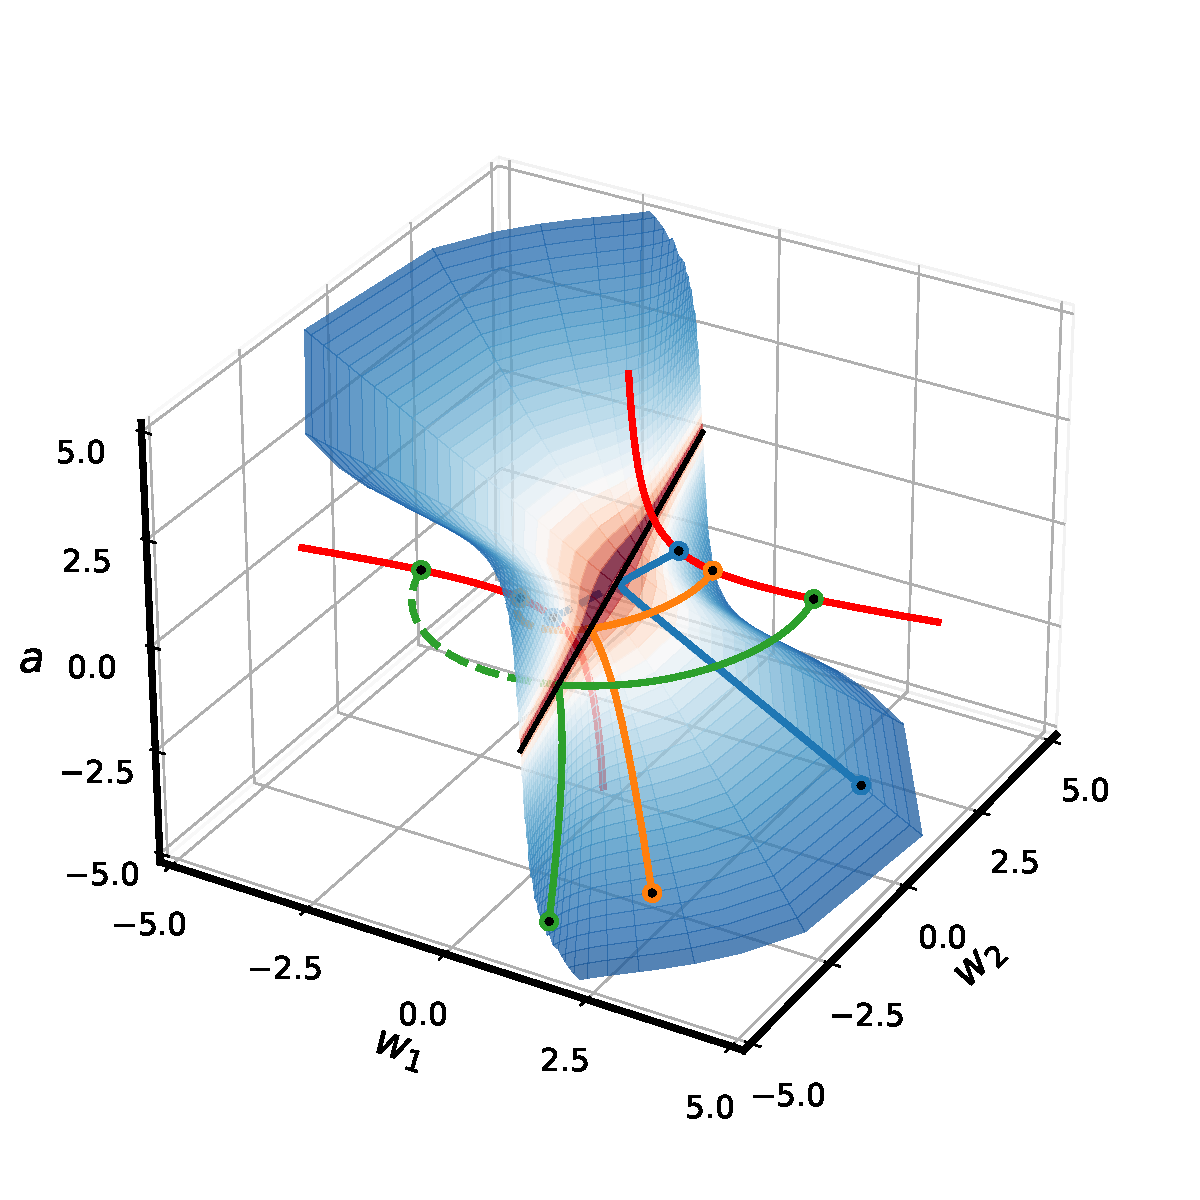
\includegraphics[width=0.5\linewidth]{fig/single-neuron/seperating-surface.pdf}
    \caption{\textbf{Two basins of attraction.}
    %
    For this model, parameter space is partitioned into two basins of attraction, one for the positive and negative branch of the minima manifold.
    %
    The surface separating the basins of attraction is determined by the equation $w_0^\intercal \beta_* + \frac{a_0}{2} \left(\delta + \sqrt{\delta^2 + 4 \|\beta_*\|^2}\right) = 0$.
    %
    For a given $\delta$, this equation describes a hyperplane through the origin.
    %
    However, a given $\delta$ can only be achieved on the surface of some hyperboloid.
    %
    Thus, the separating surface is the union of the intersections of a hyperplane and a hyperboloid, both parameterized by $\delta$.
    %
    This intersection is empty if $\delta > 0$.
    %
    Initializations exactly on the separating surface will travel along the surface to a saddle point where $w^\intercal \beta_* = a = 0$.
    }
    \label{fig:single-neuron-basins}
\end{figure}
% Could consider adding a plot of what this space of initializations that converge to saddle points looks like in function space? For a given delta should look like lines coming into origin.  Delta = 0 is line with complete negative correlation.  With \delta -> -\infty should be orthogonal line.



\subsubsection{Recovering parameters \texorpdfstring{$(a, w)$}{} from \texorpdfstring{$(\mu, \phi)$}{}}
\label{app:single-neuron-a-w-from-mu-phi}

We now discuss how to recover the dynamics of the parameters $(a, w)$ from our solutions for $(\mu, \phi)$.
%
We can recover $a$ and $\|w\|$ from $\mu$.
%
Using \cref{eq:single-neuron-key-simplification} discussed previously, we can show
%
\begin{equation}
    a = \mathrm{sgn}(\mu)\sqrt{\frac{\sqrt{\delta^2 + 4\mu^2} + \delta}{2}}, \qquad \|w\| = \sqrt{\frac{\sqrt{\delta^2 + 4\mu^2} - \delta}{2}}.
\end{equation}
%
We now discuss how to obtain the vector $w$ from $\phi$. 
%
The key observation, as discussed in \cref{sec:single-neuron}, is that $w$ only moves in the span of $w_0$ and $\beta_*$. This means we can express $w(t)$ as 
\begin{equation}
    w(t) = c_1(t)\left(\frac{\beta_*}{\|\beta_*\|}\right) + c_2(t) \left(\tfrac{\left(\mathbf{I}_d - \frac{\beta_*\beta_*^\intercal}{\|\beta_*\|^2}\right)w_0}{\sqrt{\|w_0\|^2-\left(\frac{\beta_*^\intercal w_0}{\|\beta_*\|}\right)^2}}\right)
\end{equation}
where $c_1(t)$ is the coefficient in the direction of $\beta_*$ and $c_2(t)$ is the coefficient in the direction orthogonal to $\beta_*$ on the two-dimensional plane defined by $w_0$.
%
From the definition of $\phi$ we can easily obtain the coefficients $ c_1 = \|w\|\phi$ and $c_2 = \sqrt{\|w\|^2-c_1^2}$.
%
We always choose the positive square root for $c_2$, as $c_2(t) \ge 0$ for all $t$. 
%
See \cref{app:experimental-details-single-neuron} for experimental details of how we ran our simulations and a notebook generating these exact solutions.



\begin{figure}[H]
    \centering
    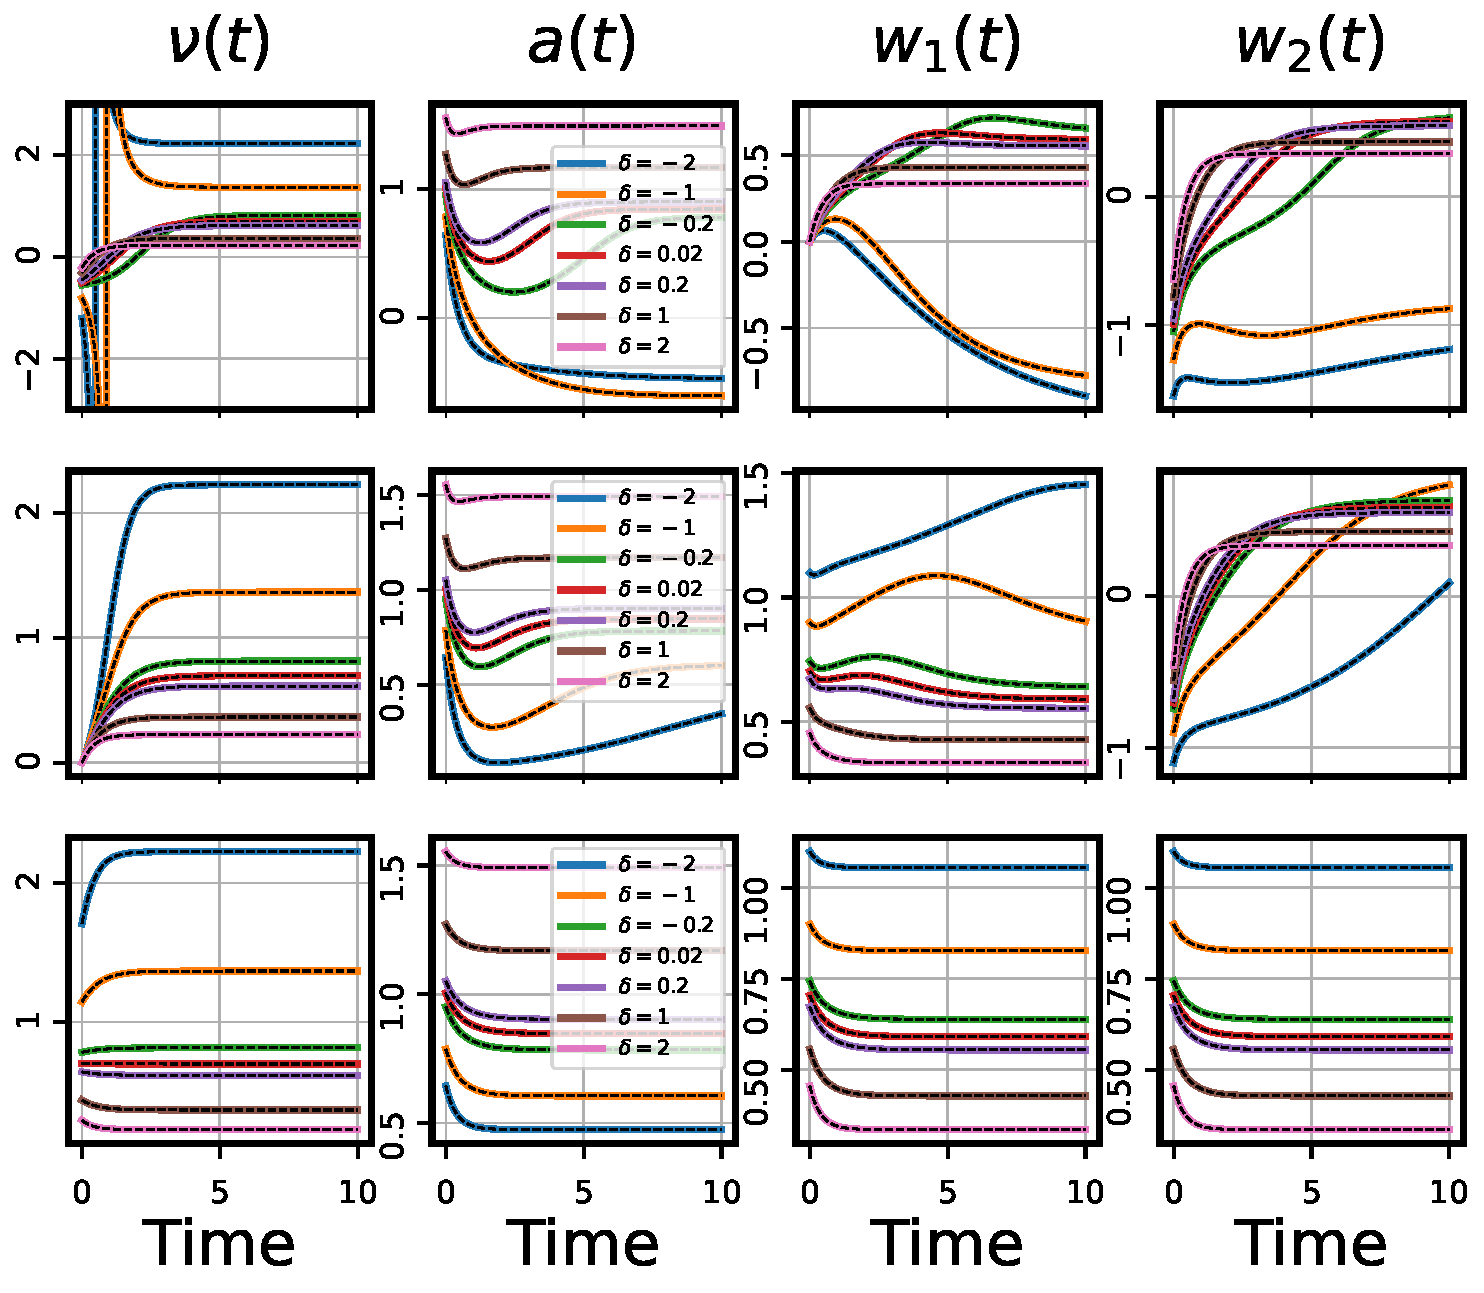
\includegraphics[width=\columnwidth]{fig/single-neuron/param_trajectories_v2.pdf}

    \caption{\textbf{Exact temporal dynamics of relevant variables in single-hidden neuron model.} Our theory recovers the time evolution under gradient flow of the quantities considered in this section, specifically $\nu$, $\varphi$, and $\zeta$, as well as the resulting dynamics of the model parameters $\{a, w_1, w_2\}$. The true $\beta*$ is a unit vector pointing in $\pi/4$ direction; $\beta(0)$ is a unit vector pointing towards $3\pi/2$, $-\pi/4$, and $\pi/4$ directions, respectively, for each of the three rows. $\delta$ then defines how $a(0)$ and $\|w(0)\|$ are chosen for a particular $\beta(0)$ where by convention we choose $a(0) > 0$.}
    \label{fig:single-neuron-trajectories}
\end{figure}




\subsection{Function space dynamics \texorpdfstring{of $\beta$}{}}
\label{app:single-neuron-beta}

The network's function is determined by the product $\beta = aw$ and governed by the ODE,
\begin{equation}
    \label{eq:single-neuron-beta}
    \dot{\beta} = a \dot{w} + \dot{a} w = -\underbrace{\left(\eta_w a^2\mathbf{I}_d + \eta_a w w^\intercal\right)}_{M} \underbrace{\left(X^\intercal X \beta - X^\intercal y\right)}_{X^\intercal \rho}.
\end{equation}
Notice, that the vector $X^\intercal \rho$ driving the dynamics of $\beta$ is the gradient of the loss with respect to $\beta$, $X^\intercal \rho = \nabla_\beta \mathcal{L}$.
%
Thus, these dynamics can be interpreted as preconditioned gradient flow on the loss in $\beta$ space where the preconditioning matrix $M$ depends on time through its dependence on $a^2$ and $ww^\intercal$.
%
The matrix $M$ also characterizes the NTK matrix, $K = XMX^\intercal$.
%
As discussed in \cref{sec:single-neuron}, our goal is to understand the evolution of $M$ along a trajectory $\{\beta(t) \in \mathbb{R}^d \;:\; t \ge 0 \}$ solving \cref{eq:single-neuron-beta}.


First, notice that by expanding $\|\beta\|^2 = a^2\|w\|^2$ in terms of the conservation law, we can show
\begin{equation}
    a^2 = \frac{\sqrt{\delta^2 + 4\eta_a\eta_w\|\beta\|^2} + \delta}{2\eta_w},
\end{equation}
which is the unique positive solution of the quadratic expression $\eta_wa^4 - \delta a^2 - \eta_a\|\beta\|^2 = 0$.
%
When $a^2 > 0$ we can use this solution and the outer product $\beta\beta^\intercal = a^2 ww^\intercal$ to solve for $ww^\intercal$ in terms of $\beta$,
\begin{equation}
    ww^\intercal = \frac{\sqrt{\delta^2 + 4\eta_a\eta_w\|\beta\|^2} - \delta}{2\eta_a}\frac{\beta\beta^\intercal}{\|\beta\|^2}.
\end{equation}
Plugging these expressions into $M$ gives
\begin{equation}
    M = \frac{\sqrt{\delta^2 + 4\eta_a\eta_w\|\beta\|^2} + \delta}{2}\mathbf{I}_d + \frac{\sqrt{\delta^2 + 4\eta_a\eta_w\|\beta\|^2} - \delta}{2}\frac{\beta\beta^\intercal}{\|\beta\|^2}.
\end{equation}

Thus, given any initialization $a_0, w_0$ such that $a(t)^2 \neq 0$ for all $t \ge 0$, we can express the dynamics of $\beta$ entirely in terms of $\beta$.
%
This is true for all initializations with $\delta \ge 0$, except if initialized on the saddle point at the origin.
%
It is also true for all initializations with $\delta < 0$ where the sign of $a$ does not switch signs.
%
In the next section we will show how to interpret these trajectories as time-warped mirror flows for a potential that depends on $\delta$.
%
As a means of keeping the analysis entirely in $\beta$ space, we will make the slightly more restrictive assumption to only study trajectories given any initialization $\beta_0$ such that $\|\beta (t)\| > 0$ for all $t \ge 0$.


Notice, that $\eta_a$ and $\eta_w$ only appear in the dynamics for $\beta$ as the product $\eta_a\eta_w$ or in the expression for $\delta$.
%
By defining $\beta' = \sqrt{\eta_a\eta_w} \beta$ and $y' = \sqrt{\eta_a\eta_w} y$ and studying the dynamics of $\beta'$, we can absorb $\eta_a\eta_w$ into the $\beta$ terms in $M$ and the additional factor $\sqrt{\eta_a\eta_w}$ into the $\beta$ and $y$ terms in $\rho$.
%
This transformation of $\beta$ and $y$ merely rescales $\beta$ space without changing the loss landscape or location of critical points. 
%
As a result, from here on we will, without loss of generality, study the dynamics of $\beta$ assuming $\eta_a\eta_w = 1$.

\subsubsection{Kernel dynamics}
\label{app:single-neuron-kernel}

The dynamics of the NTK matrix $K = X M X^\intercal$ is determined by $\dot{M}$. From \cref{eq:M_c=1}, which is derived in this section, we can write $\dot{M} = \frac{2 \|\beta\|}{\kappa} (\mathbf{I}_d + \hat{\beta}\hat{\beta}^\intercal) \partial_t \|\beta\| + \frac{\kappa - \delta}{2} \partial_t (\hat{\beta}\hat{\beta}^\intercal)$ where $\hat{\beta} = \tfrac{\beta}{\|\beta\|}$. From this expression we see that the change in $M$ is driven by two terms, one that depends on the change in the magnitude of $\beta$ and another that depends on the change in the direction of $\beta$. As done in the main text, we consider $\delta \gg 0$,  $\delta \ll 0$, and $\delta = 0$ to identify different regimes of learning. For $\delta \gg 0$, the coefficients in front of both terms vanish, and thus, irrespective of the trajectory taken from $\beta(0)$ to $\beta_*$, the change in the NTK is vanishing, indicative of a lazy regime. For $\delta \ll 0$, the coefficient for the first term vanishes, while the coefficient on the second term diverges. Here, the change in the NTK is driven solely by the change in the direction of $\beta$. This is why for large negative delta we observe a delayed rich regime, where the eventual alignment of $\beta$ to $\beta_*$ leads to a dramatic change in the kernel. When $\delta = 0$, the coefficients for both terms are roughly of the same order, and thus changes in both the magnitude and direction of $\beta$ contribute to a change in the kernel, indicative of a rich regime.



\subsection{Deriving the inductive bias}
\label{app:single-neuron-inductive-bias}


Until now, we have primarily considered that $X^\intercal X$ is either whitened or full rank, ensuring the existence of a unique least squares solution $\beta_*$.
%
In this setting, $\delta$ influences the trajectory the model takes from initialization to convergence, but all models eventually converge to the same point, as shown in \cref{fig:single-neuron-beta}.
%
Now we consider the over-parameterized setting where we have more features $d$ than observations $n$ such that $X^\intercal X$ is low-rank and there exists infinitely many interpolating solutions in function space.
%
By studying the structure of $M$ we can characterize or even predict how $\delta$ determines which interpolating solution the dynamics converge to among all possible interpolating solutions.
%
To do this we will extend a time-warped mirror flow analysis strategy pioneered by \citet{azulay2021implicit}.


\subsubsection{Overview of time-warped mirror flow analysis}
\label{app:mirror-flow-analysis}

Here we recap the standard analysis for determining the implicit bias of a linear network through mirror flow.
%
As first introduced in \citet{gunasekar2018characterizing}, if the learning dynamics of the predictor $\beta$ can be expressed as a \emph{mirror flow} for some strictly convex potential $\Phi_\alpha(\beta)$,
\begin{equation}
    \label{eq:mirror-flow}
    \dot{\beta} = -\left(\nabla^2 \Phi_\alpha(\beta)\right)^{-1} X^\intercal \rho,
\end{equation}
where $\rho = (X\beta - y)$ is the residual, then the limiting solution of the dynamics is determined by the constrained optimization problem,
\begin{equation}
    \label{eq:mirror-flow-bregman}
    \beta(\infty) = \argmin_{\beta \in \mathbb{R}^d} D_{\Phi_{\alpha}}(\beta, \beta(0)) \quad \text{s.t.} \quad  X \beta = y,
\end{equation}
where $D_{\Phi_{\alpha}}(p,q) = \Phi_{\alpha}(p) - \Phi_{\alpha}(q) - \langle \nabla \Phi_{\alpha}(q), p-q\rangle$ is the Bregman divergence defined with $\Phi_{\alpha}$.
%
To understand the relationship between mirror flow \cref{eq:mirror-flow} and the optimization problem \cref{eq:mirror-flow-bregman}, we consider an equivalent constrained optimization problem
\begin{equation}
    \label{eq:argmin-Q}
    \beta(\infty) = \argmin_{\beta \in \mathbb{R}^d} Q(\beta) \quad \text{s.t.} \quad  X \beta = y,
\end{equation}
where $Q(\beta) = \Phi_\alpha(\beta) - \nabla \Phi_\alpha(\beta(0))^\intercal \beta$, which is often referred to as the \emph{implicit bias}.
%
$Q(\beta)$ is strictly convex, and thus it is sufficient to show that $\beta(\infty)$ is a first order KKT point of the constrained optimization (\ref{eq:argmin-Q}).
%
This is true iff there exists $\nu \in \mathbb{R}^n$ such that $\nabla Q(\beta(\infty)) = X^\intercal \nu$.
%
The goal is to derive $\nu$ from the mirror flow \cref{eq:mirror-flow}.
%
Notice, we can rewrite \cref{eq:mirror-flow} as, $\dot{\left(\nabla \Phi_\alpha(\beta)\right)} = -X^\intercal \rho$, which integrated over time gives
\begin{equation}
    \nabla \Phi_\alpha(\beta(\infty)) - \nabla \Phi_\alpha(\beta(0)) = -X^\intercal\int_0^\infty \rho(t)dt.
\end{equation}
The LHS is $\nabla Q(\beta(\infty))$.
%
Thus, by defining $\nu = \int_0^\infty \rho(t)dt$, which assumes the residual decays fast enough such that this is well defined, then we have shown the desired KKT condition.
%
Crucial to this analysis is that there exists a solution to the second-order differential equation
\begin{equation}
    \nabla^2 \Phi_\alpha(\beta) = \left(\nabla_\theta \beta \nabla_\theta \beta^\intercal\right)^{-1},
\end{equation}
which even for extremely simple Jacobian maps may not be true \cite{gunasekar2021mirrorless}.
%
\citet{azulay2021implicit} showed that if there exists a smooth positive function $g(\beta) : \mathbb{R}^d \to (0,\infty)$ such that the ODE,
% Note that if g can be zero, then this could be used to generalize Theorem 3.1 to when \beta(t) = 0...could g be negative?
\begin{equation}
    \nabla^2 \Phi_\alpha(\beta) = g(\beta)\left(\nabla_\theta \beta \nabla_\theta \beta^\intercal\right)^{-1},
\end{equation}
has a solution, then the previous interpretation holds for $\Phi_\alpha(\beta)$ with $\nu = \int_0^\infty g(\beta(t'))\rho(t')dt$.
%
As before, it is crucial that this integral exists and is finite.
%
\citet{azulay2021implicit} further explained that this scalar function $g(\beta)$ can be considered as warping time $\tau(t) = \int_0^tg(\beta(t'))dt'$ on the trajectory taken in predictor space $\beta(\tau(t))$.
%
So long as this warped time doesn't ``stall out'', that is we require that $\tau(\infty) = \infty$, then this will not change the interpolating solution.


\subsubsection{Applying time-warped mirror flow analysis}

Here show how to apply the time-warped mirror flow analysis to the dynamics of $\beta$ derived in \cref{app:single-neuron-beta} where $\nabla_\theta \beta \nabla_\theta \beta^\intercal = M$.
%
We will only consider initializations $\beta_0$ such that $\|\beta(t)\| > 0$ for all $t \ge 0$, such that $M$ can be expressed as
\begin{equation}
    M = \frac{\sqrt{\delta^2 + 4\|\beta\|^2} + \delta}{2}I_d + \frac{\sqrt{\delta^2 + 4\|\beta\|^2} - \delta}{2}\frac{\beta\beta^\intercal}{\|\beta\|^2}.
\end{equation}

\textbf{Computing $M^{-1}$.}
%
Whenever $\|\beta\| > 0$, then $M$ is a positive definite matrix with a unique inverse that can be derived using the Sherman–Morrison formula, $(A + uv^\intercal)^{-1} = A^{-1} - \tfrac{A^{-1}uv^\intercal A^{-1}}{1 + u^\intercal A^{-1}v}$. Here we can define $A$, $u$, and $v$ as
\begin{equation}
    A = \left(\frac{\sqrt{\delta^2 + 4\|\beta\|^2} + \delta}{2}\right)I_d,\;
    u = \left(\frac{\sqrt{\delta^2 + 4\|\beta\|^2} - \delta}{2\|\beta\|^2}\right)\beta,\;
    v = \beta
\end{equation}
First notice the following simplification, $u^\intercal A^{-1}v = \frac{\sqrt{\delta^2 + 4\|\beta\|^2} - \delta}{\sqrt{\delta^2 + 4\|\beta\|^2} + \delta}$.
%
After some algebra, $M^{-1}$ is
\begin{equation}
    M^{-1} = \left(\frac{2}{\sqrt{\delta^2 + 4\|\beta\|^2} + \delta}\right)I_d - \left(\frac{\frac{\sqrt{\delta^2 + 4\|\beta\|^2} - \delta}{\sqrt{\delta^2 + 4\|\beta\|^2} + \delta}}{\|\beta\|^2\sqrt{\delta^2 + 4\|\beta\|^2}}\right)\beta\beta^\intercal
\end{equation}
To make notation simpler we will define the following two scalar functions,
\begin{equation}
    \label{eq:f-defn-M-inv-two-layer}
    f_\delta(x) = \frac{2}{\sqrt{\delta^2 + 4x} + \delta},\qquad
    h_\delta(x) = \frac{\sqrt{\delta^2 + 4x} - \delta}{x\sqrt{\delta^2 + 4x}\left(\sqrt{\delta^2 + 4x} + \delta\right)},
\end{equation}
such that we can express $M^{-1} = f_\delta\left(\|\beta\|^2\right)I_d - h_\delta\left(\|\beta\|^2\right)\beta\beta^\intercal$.


\textbf{Proving $M^{-1}$ is not a Hessian map.}
%
If $M^{-1}$ is the Hessian of some potential, then we can show that the dynamics of $\beta$ are a mirror flow.
%
However, from our expression for $M^{-1}$ we can actually prove that it is \emph{not} a Hessian map.
%
As discussed in \citet{gunasekar2021mirrorless}, a symmetric matrix $H(\beta)$ is the Hessian of some potential $\Phi(\beta)$ if and only if it satisfies the condition,
\begin{equation}
    \forall \beta\in \mathbb{R}^m, \quad \forall i,j,k \in [m] \quad 
    \frac{\partial H_{ij}(\beta)}{\partial \beta_k } = \frac{\partial H_{ik}(\beta)}{\partial \beta_j }.
\end{equation}
We will use this property to show $M^{-1}$ is not a Hessian map.
%
First, notice this condition is trivially true when $i = j = k$.
%
Second, notice that for all $i \neq j \neq k$,  
\begin{equation}
    \frac{\partial M^{-1}_{ij}}{\partial \beta_k } = \frac{\partial M^{-1}_{ik}}{\partial \beta_j } = -2\nabla h_\delta\left(\|\beta\|^2\right) \beta_i\beta_j\beta_k
\end{equation}
Thus, $M^{-1}$ is a Hessian map if and only if for all $i \neq j$, $\frac{\partial M^{-1}_{ii}}{\partial \beta_j} = \frac{\partial M^{-1}_{ij}}{\partial \beta_i}$.
%
Using our expression for $M^{-1}$, the LHS is
\begin{equation}
    \frac{\partial M^{-1}_{ii}}{\partial \beta_j} = 2\nabla f_\delta\left(\|\beta\|^2\right) \beta_j - 2\nabla h_\delta\left(\|\beta\|^2\right) \beta_j\beta_i^2
\end{equation}
while the RHS is
\begin{equation}
    \frac{\partial M^{-1}_{ij}}{\partial \beta_i} = -h_\delta\left(\|\beta\|^2\right) \beta_j - 2\nabla h_\delta\left(\|\beta\|^2\right) \beta_j\beta_i^2
\end{equation}
Thus, $M^{-1}$ is a Hessian map if and only if $2\nabla f_\delta(x) + h_\delta(x) = 0$.
%
Plugging in our definitions of $f_\delta(x)$ and $h_\delta(x)$ we find
\begin{equation}
    \label{eq:hessian-condition-f-h}
    2\nabla f_\delta(x) + h_\delta(x) = \frac{-4}{\sqrt{\delta^2 + 4x}(\sqrt{\delta^2 + 4x} + \delta)^2},
\end{equation}
which does not equal zero and thus $M^{-1}$ is not a Hessian map.
% The gradient $\nabla f_\delta(x)$ is
% \begin{equation}
%     \nabla f_\delta(x) = \frac{-4}{\sqrt{\delta^2 + 4x}(\sqrt{\delta^2 + 4x} + \delta)^2},
% \end{equation}



\textbf{Finding a scalar function $g_\delta(x)$ such that $g_\delta(\|\beta\|^2)M^{-1}$ is a Hessian map.}
%
While we have shown that $M^{-1}$ is not a Hessian map, it is very close to a Hessian map.
%
Here we will show that there exists a scalar function $g_\delta(x)$ such that $g_\delta\left(\|\beta\|^2\right)M^{-1}$ is a Hessian map.
%
For any $g_\delta(x)$ can define $g_\delta\left(\|\beta\|^2\right)M^{-1}$ in terms of two new functions $\tilde{f}_\delta(x)$ and $\tilde{h}_\delta(x)$ evaluated at $x = \|\beta\|^2$,
\begin{equation}
    g_\delta\left(\|\beta\|^2\right)M^{-1} = \underbrace{g_\delta\left(\|\beta\|^2\right)f_\delta\left(\|\beta\|^2\right)}_{\tilde{f}_\delta\left(\|\beta\|^2\right)}I_d - \underbrace{g_\delta\left(\|\beta\|^2\right)h_\delta\left(\|\beta\|^2\right)}_{\tilde{h}_\delta\left(\|\beta\|^2\right)}\beta\beta^\intercal.
\end{equation}
Thus, as derived in the previous section, we get the analogous condition on $\tilde{f}_\delta(x)$ and $\tilde{h}_\delta(x)$ for $g_\delta\left(\|\beta\|^2\right)M^{-1}$ to be a Hessian map,
\begin{equation}
    2 \underbrace{\left(\nabla g_\delta(x) f_\delta(x) + g(x)\nabla f_\delta(x)\right)}_{\nabla \tilde{f}_\delta(x)} + \underbrace{g_\delta(x)h_\delta(x)}_{\tilde{h}_\delta(x)} = 0
\end{equation}
Rearranging terms we find that $g_\delta(x)$ must solve the ODE
\begin{equation}
    \nabla g_\delta(x) = -\left(2f_\delta(x)\right)^{-1}\left(2\nabla f_\delta(x) + h_\delta(x)\right)g_\delta(x).
\end{equation}
Using our previous expressions (\cref{eq:f-defn-M-inv-two-layer} and \cref{eq:hessian-condition-f-h}) we find
\begin{equation}
-\left(2f_\delta(x)\right)^{-1}\left(2\nabla f_\delta(x) + h_\delta(x)\right) = \frac{1}{\sqrt{\delta^2 + 4x}(\sqrt{\delta^2 + 4x} + \delta)},
\end{equation}
which implies $g_\delta(x)$ solves the differential equation, $\nabla g_\delta(x) = \frac{g_\delta(x)}{\sqrt{\delta^2 + 4x}(\sqrt{\delta^2 + 4x} + \delta)}$.
%
The solution is $g_\delta(x) = c\sqrt{\sqrt{\delta^2 + 4x} + \delta}$, where $c \in \mathbb{R}$ is a constant.
%
Let $c = 1$.
%
Plugging in our expressions for $g_\delta\left(\|\beta\|^2\right)$, $f_\delta\left(\|\beta\|^2\right)$, $h_\delta\left(\|\beta\|^2\right)$, we get that
\begin{equation}
    \label{eq:g-m-inv-two-layer}
    g_\delta\left(\|\beta\|^2\right)M^{-1} = \left(\frac{2}{\sqrt{\sqrt{\delta^2 + 4\|\beta\|^2} + \delta}}\right)I_d - \left(\frac{\frac{\sqrt{\delta^2 + 4\|\beta\|^2} - \delta}{\sqrt{\sqrt{\delta^2 + 4\|\beta\|^2} + \delta}}}{\|\beta\|^2\sqrt{\delta^2 + 4\|\beta\|^2}}\right)\beta\beta^\intercal
\end{equation}
is a Hessian map for some unknown potential $\Phi_\delta(\beta)$.



\textbf{Solving for the potential $\Phi_\delta(\beta)$.}
%
Take the ansatz that there exists some function scalar $q(x)$ such that $\Phi_\delta(\beta) = q_\delta(\|\beta\|) + c_\delta$ where $c_\delta$ is a constant such that $\Phi_\delta(\beta) > 0$ for all $\beta \neq 0$ and $\Phi_\delta(0) = 0$.
%
The Hessian of this ansatz takes the form,
\begin{equation}
    \nabla^2 \Phi_\delta(\beta) = \left(\frac{\nabla q(\|\beta\|)}{\|\beta\|}\right) I_d - \left(\frac{\nabla q(\|\beta\|)}{\|\beta\|^{3}} - \frac{\nabla^2 q(\|\beta\|)}{\|\beta\|^2}\right)\beta\beta^\intercal.
\end{equation}
Equating terms from our expression for $g_\delta\left(\|\beta\|^2\right)M^{-1}$ (equation~\ref{eq:g-m-inv-two-layer}) we get the expression for $\nabla q(\|\beta\|)$
\begin{equation}
    \label{eq:gradient-condition-two-layer}
    \nabla q(\|\beta\|) = \frac{2\|\beta\|}{\sqrt{\sqrt{\delta^2 + 4\|\beta\|^2} + \delta}},
\end{equation}
which plugged into the second term gives the expression for $\nabla^2 q(\|\beta\|)$,
\begin{equation}
    \label{eq:hessian-condition-two-layer}
    \nabla^2 q(\|\beta\|) = \frac{2}{\sqrt{\sqrt{\delta^2 + 4\|\beta\|^2} + \delta}} - \left(\frac{\frac{\sqrt{\delta^2 + 4\|\beta\|^2} - \delta}{\sqrt{\sqrt{\delta^2 + 4\|\beta\|^2} + \delta}}}{\sqrt{\delta^2 + 4\|\beta\|^2}}\right) = \frac{\sqrt{\sqrt{\delta^2 + 4\|\beta\|^2} + \delta}}{\sqrt{\delta^2 + 4\|\beta\|^2}}.
\end{equation}
%
We now look for a function $q(x)$ such that both these conditions (\cref{eq:gradient-condition-two-layer} and \cref{eq:hessian-condition-two-layer}) are true.
%
Consider the following function and its derivatives,
\begin{align}
    q(x) &= \frac{1}{3}\left(\sqrt{\delta^2 + 4x^2} - 2\delta\right)\sqrt{\sqrt{\delta^2 + 4x^2} + \delta}\\
    \nabla q(x) &= \frac{2x}{\sqrt{\sqrt{\delta^2 + 4x^2} + \delta}}\\
    \nabla^2 q(x) &= \frac{\sqrt{\sqrt{\delta^2 + 4x^2} + \delta}}{\sqrt{\delta^2 + 4x^2}}
\end{align}
Letting $x = \|\beta\|$ notice $\nabla q(\|\beta\|)$ and $\nabla^2 q(\|\beta\|)$ satisfies the previous conditions.
%
Furthermore, $\nabla^2 q(x) > 0$ for all $\delta$ as long as $x \neq 0$ and thus $q(x)$ is a convex function which achieves its minimum at $x = 0$. 
%
Thus, the constant $c_\delta = -q(0)$ is
\begin{equation}
    c_\delta = 
    \begin{cases}
        0 & \text{if } \delta \le 0\\
        \frac{\sqrt{2}|\delta|^\frac{3}{2}}{3} & \text{if } \delta > 0
    \end{cases} = \max\left(0, \mathrm{sgn}(\delta)\frac{\sqrt{2}|\delta|^\frac{3}{2}}{3}\right),
\end{equation}
and the potential $\Phi_\delta(\beta)$ is 
\begin{equation}
    \Phi_\delta(\beta) = \frac{1}{3}\left(\sqrt{\delta^2 + 4\|\beta\|^2} - 2\delta\right)\sqrt{\sqrt{\delta^2 + 4\|\beta\|^2} + \delta} + \max\left(0, \mathrm{sgn}(\delta)\frac{\sqrt{2}|\delta|^\frac{3}{2}}{3}\right).
\end{equation}
%Finally, putting it all together, we can express the inductive bias in the following theorem:
% \begin{theorem}
%     \label{thrm:single-neuron-implicit-bias}
%     For a two-layer linear network with a single hidden neuron ($h = 1$), any $\delta \in \mathbb{R}$, and initialization $\beta_0$ such that $\|\beta(t)\| > 0$ for all $t \ge 0$, if the gradient flow solution $\beta(\infty)$ satisfies $X \beta(\infty) = y$, then,
%     \begin{equation}
%         \beta(\infty) = \argmin_{\beta \in \mathbb{R}^d} \Psi_\delta(\beta) - \psi_\delta \tfrac{\beta_0}{\|\beta_0\|}^\intercal \beta \quad \mathrm{s.t.} \quad X \beta = y
%     \end{equation}
%     where $\Psi_\delta(\beta) = \frac{1}{3}\left(\sqrt{\delta^2 + 4\|\beta\|^2} - 2\delta\right)\sqrt{\sqrt{\delta^2 + 4\|\beta\|^2} + \delta}$ and $\psi_\delta = \sqrt{\sqrt{\delta^2 + 4\|\beta_0\|^2} - \delta}$.
% \end{theorem}
Finally, putting it all together, we can express the inductive bias as in \cref{thrm:single-neuron-implicit-bias}.

\subsubsection{Connection to Theorem 2 in \texorpdfstring{\citet{azulay2021implicit}}{Azulay et al.}}

We discuss how \cref{thrm:single-neuron-implicit-bias} connects to Theorem 2 in \citet{azulay2021implicit}, which we rewrite:

\begin{theorem}[Theorem 2 from \citet{azulay2021implicit}]
    \label{thrm:single-neuron-azulay}
    For a depth 2 fully connected network with a single hidden neuron ($h = 1$), any $\delta \ge 0$, and initialization $\beta_0$ such that $\beta_0 \neq 0$, if the gradient flow solution $\beta(\infty)$ satisfies $X \beta(\infty) = y$, then,
    \begin{equation}
        \beta(\infty) = \argmin_{\beta \in \mathbb{R}^d} q_\delta(\|\beta\|) + z^\intercal \beta \quad \mathrm{s.t.} \quad X \beta = y
    \end{equation}
    where $q_\delta(x) = \frac{\left(x^2 - \frac{\delta}{2}\left(\frac{\delta}{2} + \sqrt{x^2 + \frac{\delta^2}{4}}\right)\right)\sqrt{\sqrt{x^2 + \frac{\delta^2}{4}} - \frac{\delta}{2}}}{x}$ and $z = -\frac{3}{2}\sqrt{\sqrt{\|\beta_0\|^2 + \frac{\delta^2}{4}} - \frac{\delta}{2}} \frac{\beta_0}{\|\beta_0\|}$.
\end{theorem}

The most striking difference is in the expressions for the inductive bias.
%
\citet{azulay2021implicit} take an alternative route towards deriving the inductive bias by inverting $M$ in terms of the original parameters $a$ and $w$ and then simplifying $M^{-1}$ in terms of $\beta$, which results in quite a different expression for their inductive bias.
%
However, they are actually functionally equivalent.
%
It requires a bit of algebra, but one can show that
\begin{equation}
    \Phi_\delta(\beta) =  \frac{2\sqrt{2}}{3}q_\delta(\|\beta\|) + c_\delta.
\end{equation}
%
% Steps not presented:
% 1. Multiply and divide $q_\delta(\|\beta\|)$ by $\sqrt{\sqrt{\delta^2/4 + \|\beta\|^2} + \delta / 2}$
% 2. Divide the \|\beta\|^2 term by the same factor and turn expression into a product of two terms
% 3. Multiply and divide first term by $\sqrt{\delta^2/4 + \|\beta\|^2} - \delta / 2$
% 4. Multiply by 2\sqrt{2} / 3 and clean up constants
%
Another important distinction between our two theorems lies in the assumptions we make.
%
\citet{azulay2021implicit} consider only initializations such that $\delta \ge 0$ and $\beta_0 \neq 0$. 
%
We make a less restrictive assumption by considering initializations $\beta_0$ such that $\|\beta(t)\| > 0$ for all $t \ge 0$, which allows for both positive and negative $\delta$.
%
Except for a measure zero set of initializations, all initializations considered by \citet{azulay2021implicit} also satisfy our assumptions.
%
In both cases, our assumptions ensure that $M$ is invertible for the entire trajectory from initialization to interpolating solution. 
%
However, it is worth considering whether the theorems would hold even when there exists a point on the trajectory where $M$ is low-rank. 
%
As discussed in \cref{app:single-neuron-beta}, this can only happen for an initialization with $\delta < 0$ and where the sign of $a$ changes.
%
Only at the point where $a(t) = 0$ does $M$ become low-rank.
%
A similar challenge arose in this setting when deriving the exact solutions presented in \cref{app:single-neuron-negative}. 
%
We were able to circumvent the issue in part by introducing \cref{lemma:crossing} proving that this sign change could only happen at most once given any initialization.
%
This lemma was based on the setting with whitened input, but a similar statement likely holds for the general setting.
%
If this were the case, we could define $M$ at this unique point on the trajectory in terms of the limit of $M$ as it approached this point. 
%
This could potentially allow us to extend the time-warped mirror flow analysis to all initializations such that $\|\beta_0\| > 0$.



\subsubsection{Exact solution when interpolating manifold is one-dimensional}

When the null space of $X^\intercal X$ is one-dimensional, the constrained optimization problems in \cref{thrm:single-neuron-implicit-bias} and \cref{thrm:single-neuron-azulay} have an exact analytic solution.
%
In this case we can parameterize all interpolating solutions $\beta$ with a single scalar $\alpha \in \mathbb{R}$ such that $\beta = \beta_* + \alpha v$ where $X^\intercal X v = 0$ and $\|v\| = 1$.
%
Using this description of $\beta$, we can then differentiate the inductive bias with respect to $\alpha$, set to zero, and solve for $\alpha$.
%
We will use the following expressions,
\begin{equation}
    \nabla_x q(x) = \frac{3}{2}\mathrm{sign}(x)\sqrt{\sqrt{x^2 + \frac{\delta^2}{4}} - \frac{\delta}{2}}, \quad
    \nabla_\alpha \|\beta\| = \frac{\alpha}{\|\beta\|}, \quad
    \nabla_\alpha z^\intercal \beta = z^\intercal v.
\end{equation}
We will also use the expression, $\|\beta\|^2 = \|\beta_*\|^2 + \alpha^2$.
%
Pulling these expressions together we get the following equation for $\alpha$,
\begin{equation}
    \sqrt{\sqrt{\|\beta_*\|^2 + \alpha^2 + \frac{\delta^2}{4}} - \frac{\delta}{2}} \frac{\alpha}{\sqrt{\|\beta_*\|^2 + \alpha^2}} = -\frac{2z^\intercal v}{3}.
\end{equation}
If we let $k = -\frac{2z^\intercal v}{3}$, the solution for $\alpha$ is
\begin{equation}
    \alpha = k \sqrt{\frac{k^2 + \delta}{2} + \sqrt{\left(\frac{k^2 + \delta}{2}\right)^2 + \|\beta_*\|^2}}.
\end{equation}
This solution always works for the initializations we considered in \cref{thrm:single-neuron-implicit-bias}. 
%
Interestingly, it appears that $\beta = \beta_* - \alpha v$ also works for initializations not previously considered. 
%
This includes trajectories that pass through the origin, resulting in a change in the sign of $a$.



\clearpage
\section{Wide and Deep Linear Networks}
\label{app:wide-deep-linear-network}


Here we discuss how our analysis techniques, developed in the previous section for a single-neuron linear network, can be extended to linear networks with multiple neurons, outputs, and layers.


\subsection{Wide linear networks}

We consider the dynamics of a two-layer linear network with $h$ hidden neurons and $c$ outputs, $f(x;\theta) = A^\intercal W x$, where $W \in \mathbb{R}^{h \times d}$ and $A \in \mathbb{R}^{h \times c}$.
%
We assume that $h \ge \min(d,c)$, such that this parameterization can represent all linear maps from $\mathbb{R}^d \to \mathbb{R}^c$.
%
As in the single-neuron setting, the rescaling symmetry in this model between the first and second layer implies the $h \times h$ matrix $\Delta =  A_0A_0^\intercal - W_0W_0^\intercal$ determined at initialization remains conserved throughout gradient flow \cite{du2018algorithmic}.
%
This can be easily shown from the temporal dynamics of $A$ and $W$,
\begin{align}
    \label{eq:ODE-A-wide}
    \dot{A} &= - \eta_a W X^{\intercal} (X \beta -Y),\\
    \label{eq:ODE-W-wide}
    \dot{W}^{\intercal} &= -\eta_wX^\intercal (X\beta -Y)A^{\intercal}.
\end{align}
%
Extending derivations in \cite{braun2022exact}, the NTK matrix can be expressed as 
\begin{equation}
    K = \left(\mathbf{I}_{c} \otimes X\right)\left(\eta_w A^{\intercal}A \oplus \eta_a W^{\intercal}W\right)\left(\mathbf{I}_{c} \otimes X^\intercal\right),
\end{equation}
% The derivation used the Kronecker property {\displaystyle (\mathbf {A} \otimes \mathbf {B} )(\mathbf {C} \otimes \mathbf {D} )=(\mathbf {AC} )\otimes (\mathbf {BD} ).}
where $\otimes$ and $\oplus$ denote the Kronecker product and sum respectively.
%
The Kronecker sum is defined for square matrices $C \in \mathbb{R}^{c \times c}$ and $D \in \mathbb{R}^{d \times d}$ as $C \oplus D = C \otimes \mathbf{I}_{d} + \mathbf{I}_{c} \otimes D$.

\subsubsection{Parameter space dynamics}

Inspired by our analysis of the single-neuron setting, we introduce two coordinate transformations to study the parameter space dynamics of a wide two-layer linear network.
%
In both analyses we assume whitened input $X^\intercal X = \mathbf{I}_d$ and let $\eta_a = \eta_w = 1$.
%
However, we will find that the analysis of the dynamics in function space, for general unwhitened data, is more tractable.

\textbf{Parameter dynamics when $c = 1$.}
%
Drawing insights from our analysis of the single-neuron scenario ($h = c = 1$), we might consider a combination of hyperbolic and spherical coordinate transformations to study the parameter space dynamics of a wide two-layer linear network.
%
We consider the following two quantities for each hidden neuron $k \in [h]$:
\begin{equation}
    \mu_k = a_k\|w_k\|, \qquad \phi_k = \frac{w_k^\intercal \beta_*}{\|w_k\|\|\beta_*\|}.
\end{equation}
We will also consider a new matrix quantity $Q \in \mathbb{R}^{h\times h}$ with elements $Q_{kk'} = \frac{w_k^\intercal w_{k'}}{\|w_k\|\|w_{k'}\|}$.
%
The resulting dynamics for $\mu$ and $\phi$ can be entirely written in terms $\mu, \phi, \Delta$:
\begin{align}
    \dot{\mu} &= \sqrt{\mathrm{Diag}(\Delta)^2 + 4\mathrm{Diag}(\mu)^2}\left(\phi - Q\mu\right),\\
    \dot{\phi} &= M\mathrm{Diag}(\mu)\left((\|\beta_*\|^2 - \phi^\intercal \mu)I_h + \mathrm{Diag}(\phi)Q\mu - \phi^2\right),
\end{align}
where $M = 2\left(\sqrt{\mathrm{Diag}(\Delta)^2 + 4 \mathrm{Diag}(\mu)^2} - \mathrm{Diag}(\Delta)\right)^{-1}$.
%
Using the conserved structure of $\Delta$ we can express $Q$ as a function of $\mu$ and $M$,
\begin{equation}
    Q = M \mu \mu^\intercal M - M^{1/2}\Delta M^{1/2}.
\end{equation}
This approach yields a coupled nonlinear dynamical system with $2h$ variables.
%
Imposing additional assumptions on the initialization, such as permutation invariance between hidden neurons, can simplify the system of differential equations.
%
A similar approach was used by \citet{saad1995exact} to derive a set of differential equations for a soft committee machine model, capturing its online learning dynamics in a teacher-student setup, which \citet{goldt2019generalisation} extended to its generalization error dynamics.

\textbf{Parameter dynamics when $c = h$.}
%
In this analysis we assume an initialization such that the conserved quantities $\Delta = \delta \mathbf{I}_h$, an assumption we will discuss further in \cref{app:simplifying-assumptions-Delta}, and that $A$ is invertible throughout training.
%
Let $\beta_* = X^\intercal Y$, which for whitened input, is the unique minimum of the dynamics in function space.
%
% We consider the variable $\omega = W \beta_*$, which evolves according to
% \begin{equation}
%     \dot{\omega} = \dot{W}\beta_* 
%     = \left(AY^\intercal X - AA^\intercal W\right)\beta_* 
%     = A\beta_*^\intercal\beta_* - AA^\intercal \omega.
% \end{equation}
%
We consider the variable $\nu = A^{-1} W \beta_* \in \mathbb{R}^{c \times c}$.
%
Using the identity that $\dot{A^{-1}} = - A^{-1} \dot{A} A^{-1}$ and our assumption on $\Delta$, we find that the matrix $\nu$ evolves according to the matrix Riccati ODE,
\begin{equation}
    \dot{\nu} = \beta_*^\intercal\beta_* - \delta \nu - \nu^2.
\end{equation}
% \begin{align}
%     \dot{\nu} &= A^{-1}\dot{\omega} + \dot{A^{-1}} \omega\\
%     &= A^{-1}\left(A\beta_*^\intercal\beta_* - AA^\intercal \omega\right) - A^{-1} \left(\omega - WW^\intercal A\right) A^{-1} \omega\\
%     &= \left(\beta_*^\intercal\beta_* - A^\intercal \omega\right) + A^{-1} (AA^\intercal - \delta \mathbf{I}_h)A A^{-1}\omega - (A^{-1}\omega)^2 \\
%     &= \beta_*^\intercal\beta_* - A^\intercal \omega + A^\intercal \omega - \delta A^{-1} \omega - (A^{-1}\omega)^2\\
%     &= \beta_*^\intercal\beta_* - \delta \nu - \nu^2
% \end{align}
Additionally, consider the variable $C = A^\intercal A$, which evolves according to the matrix Bernoulli ODE
\begin{equation}
    \dot{C} = C (\nu + \delta \mathbf{I}_h) +(\nu + \delta \mathbf{I}_h)^\intercal C  - 2C^2.
\end{equation}
% \begin{align}
%     \dot{C} &= A^\intercal \dot{A} + \dot{A}^\intercal A\\ 
%     &= A^\intercal \left(W X^\intercal Y - WW^\intercal A\right) + \left(W X^\intercal Y - WW^\intercal A\right)^\intercal A\\
%     &= A^\intercal \omega + \omega^\intercal A - 2A^\intercal(AA^\intercal - \delta \mathbf{I}_h) A\\
%     &= A^\intercal A A^{-1} \omega + \omega^\intercal A^{-\intercal} A^\intercal A + 2\delta A^\intercal A - 2\left(A^\intercal A\right)^2\\
%     &= C (\nu + \delta \mathbf{I}_h) +(\nu + \delta \mathbf{I}_h)^\intercal C  - 2C^2
% \end{align}
Taken together we have found a change of variables, analogous to the one introduced in \cref{app:single-neuron-positive} for the single-neuron setting, that evolves according to a matrix Riccati and Bernoulli equation,
\begin{align}
    \dot{\nu} &= \beta_*^\intercal\beta_* - \delta \nu - \nu^2, && \nu(0) = A_0^{-1}W_0\beta_*,\\
    \dot{C} &= C (\nu + \delta \mathbf{I}_h) + (\nu + \delta \mathbf{I}_h)^\intercal C - 2C^2, && C(0) = A_0^\intercal A_0.
\end{align}
However, solving this system exactly as we did in the single-neuron setting is challenging. Unless we assume that $\nu$ and $\beta_*^\intercal\beta_*$ share the same eigenspace -- allowing us to decouple the dynamics of $\nu$ into a set of scalar Riccati equations -- the system cannot be easily solved.
%
Instead, we will find that the dynamics of the product $W^\intercal A$ in function space is more tractable and requires fewer assumptions.

\subsubsection{Function space dynamics}
%
We consider the dynamics of $\beta = W^\intercal A \in \mathbb{R}^{d \times c}$ in function space, which is governed by the ODE,
\begin{equation}
\label{eq:two-layer-beta-dynamics-AA-WW}
    \dot{\beta}=W^{\intercal}\dot{A} + \dot{W}^{\intercal}A = -\left(\eta_w X^\intercal(X \beta -Y)A^{\intercal}A + \eta_a W^{\intercal}W X^{\intercal}  (X\beta -Y)\right).
\end{equation}
%
Vectorizing using the identity  $ \mathrm{vec}(ABC) = ( C^{\intercal}\otimes A ) \mathrm{vec}(B)$ equation \ref{eq:two-layer-beta-dynamics-AA-WW} becomes
 \begin{align}
    \mathrm{vec}\left(\dot{\beta}\right) &= - \mathrm{vec} \left ( \eta_w \mathbf{I}_d X^\intercal(X \beta -Y)A^{\intercal}A  +  \eta_a W^{\intercal}W X^{\intercal} (X \beta -Y)\mathbf{I}_c \right ),\\
    &=  -( \eta_w A^{\intercal}A \otimes  \mathbf{I}_d  +  \eta_a \mathbf{I}_c \otimes W^{\intercal}W  )\mathrm{vec}(X^\intercal X\beta - X^\intercal Y),\\
    \label{eq:vect_beta}
    & =  -  \underbrace{\left(\eta_w A^{\intercal}A \oplus \eta_a W^{\intercal}W\right)}_{M} \mathrm{vec}(X^\intercal X\beta - X^\intercal Y).
\end{align}
As in the single-neuron setting, we find that the dynamics of $\beta$ can be expressed as gradient flow preconditioned by a matrix $M$ that depends on quadratics of $A$ and $W$.


\subsubsection{Proving \texorpdfstring{\cref{thrm:vec_beta}}{}}

We first prove \cref{thrm:vec_beta}.
%
Consider a single hidden neuron $k \in [h]$ of the multi-output model defined by the parameters $w_k \in \mathbb{R}^d$ and $a_k \in \mathbb{R}^c$.
%
Let $\beta_k = w_ka_k^\intercal$ be the $\mathbb{R}^{d \times c}$ matrix representing the contribution of this hidden neuron to the input-output map of the network $\beta = \sum_{k=1}^h \beta_k$.
%
Consider the two gram matrices $\beta_k^\intercal \beta_k \in \mathbb{R}^{c \times c}$ and $\beta_k \beta_k^\intercal \in \mathbb{R}^{d \times d}$,
\begin{equation}
    \beta_k^\intercal \beta_k = \|w_k\|^2 a_ka_k^\intercal, \qquad \beta_k\beta_k^\intercal = \|a_k\|^2 w_kw_k^\intercal.
\end{equation}
Notice that we can express $\|\beta_k\|_F^2$ as
\begin{equation}
    \|\beta_k\|_F^2 = \mathrm{Tr}(\beta_k^\intercal\beta_k) = \mathrm{Tr}(\beta_k\beta_k^\intercal) =  \|a_k\|^2\|w_k\|^2
\end{equation}
%
At each hidden neuron we have the conserved quantity\footnote{As long as $c > 1$, then the surface of this $d + c$ hyperboloid is always connected, however its topology will depend on the relationship between $d$ and $c$.} $\eta_w \|a_k\|^2 - \eta_a\|w_k\|^2 = \delta_k$ where $\delta_k \in \mathbb{R}$.
%
Using this quantity we can invert the expression for $\|\beta_k\|_F^2$ to get
\begin{align}
    \|a_k\|^2 &= \frac{\sqrt{\delta_k^2 + 4\eta_a \eta_w\|\beta_k\|_F^2} + \delta_k}{2\eta_w},\\
    \|w_k\|^2 &= \frac{\sqrt{\delta_k^2 + 4\eta_a \eta_w\|\beta_k\|_F^2} - \delta_k}{2\eta_a}.
\end{align}
When $\|\beta_k\|_F^2 > 0$, we can use these expressions to solve for the outer products $a_ka_k^\intercal$ and $w_kw_k^\intercal$ in terms of $\beta_k$ and $\delta_k$,
\begin{align}
    a_ka_k^\intercal &= \frac{\sqrt{\delta_k^2 + 4\eta_a \eta_w \|\beta_k\|_F^2} + \delta_k}{2\eta_w} \frac{\beta_k^\intercal\beta_k}{\|\beta_k\|_F^2},\\
    w_kw_k^\intercal &= \frac{\sqrt{\delta_k^2 + 4\eta_a \eta_w \|\beta_k\|_F^2} - \delta_k}{2\eta_a} \frac{\beta_k\beta_k^\intercal}{\|\beta_k\|_F^2}.
\end{align}
By substituting these expressions into the decompositions $A^\intercal A = \sum_{k=1}^h a_ka_k^\intercal$ and $W^\intercal W = \sum_{k=1}^h w_k w_k^\intercal$, we derive the representation for $M$ presented in \cref{thrm:vec_beta}: $M = \sum_{k = 1}^h M_k$ where
\begin{equation}
    M_k = \left(\frac{\sqrt{\delta_k^2 + 4\eta_a\eta_w\|\beta_k\|_F^2} + \delta_k}{2}\right)\frac{\beta_k^\intercal\beta_k}{\|\beta_k\|_F^2} \oplus \left(\frac{\sqrt{\delta_k^2 + 4\eta_a\eta_w\|\beta_k\|_F^2} - \delta_k}{2}\right)\frac{\beta_k\beta_k^\intercal}{\|\beta_k\|_F^2}.
\end{equation}


\subsubsection{Understanding \texorpdfstring{$M$}{} when there is a single-neuron \texorpdfstring{$h = 1$}{}}
\label{app:wide-deep-linear-network-single-neuron}

When there is a single-hidden neuron $h = \min (d, c) = 1$, the expression for $M$ presented in \cref{thrm:vec_beta} simplifies allowing us to precisely understand the influence of $\delta$ on the learning regime.
%
When $h = c = 1 $, then $\frac{\beta^\intercal\beta}{\|\beta\|_F^2} = 1$.
%
Therefore, \cref{eq:Mi} simplifies to
\begin{equation}
        M = \frac{\sqrt{\delta^2 + \eta_a \eta_w 4\|\beta\|^2} + \delta}{2}\mathbf{I}_d + \frac{\sqrt{\delta^2 + \eta_a \eta_w 4\|\beta\|^2} - \delta}{2}\frac{\beta\beta^\intercal}{\|\beta\|^2},
\end{equation}
and we recover \cref{eq:M_c=1} presented in \cref{sec:single-neuron}.
%
When $h = d = 1 $, then $\frac{\beta\beta^\intercal}{\|\beta\|_F^2} = 1$ and thus \cref{eq:Mi} simplifies to,
\begin{equation}
        M = \frac{\sqrt{\delta^2 + \eta_a \eta_w 4\|\beta\|^2} + \delta}{2}\frac{\beta^\intercal\beta}{\|\beta\|^2} + \frac{\sqrt{\delta^2 + \eta_a \eta_w 4\|\beta\|^2} - \delta}{2}\mathbf{I}_c.
\end{equation}
In both settings, $M$ is the weighted sum of the identity matrix and a rank-one projection matrix.
%
While these equations are strikingly similar there is an interesting distinction that arises in the limits of $\delta$.
%
As $\delta \to \infty$, then the first expression for $M$ becomes proportional to $\mathbf{I}_d$, while the second expression for $M$ becomes proportional to the rank-1 projection $\frac{\beta^\intercal\beta}{\|\beta\|^2}$.
%
Conversely, as $\delta \to -\infty$, then the first expression for $M$ becomes proportional to the rank-1 projection $\frac{\beta\beta^\intercal}{\|\beta\|^2}$, while the second expression for $M$ becomes proportional to $\mathbf{I}_c$. 
%
When $h = d = c = 1$, then $M = \sqrt{\delta^2 + \eta_a \eta_w 4\|\beta\|^2}$ and thus in both limits of $\delta \to \pm \infty$, $M$ becomes a constant independent of $\beta$.
%
In all settings, when $\delta = 0$, $M$ depends on $\beta$.
%
In other words, the influence of $\delta$ on whether the dynamics are lazy, rich, or delayed rich, crucially depends on the relative sizes of dimensions $d$, $h$, and $c$.





\subsubsection{Interpreting \texorpdfstring{$M$}{} in different limits and architectures}
\label{app:wide-deep-linear-network-architectures}

We now seek to more generally understand the influence of the conserved quantities $\delta_i$ and the relative sizes of dimensions $d$, $h$ and $c$ on the learning regime.
%
For a matrix $A \in \mathbb{R}^{d \times c}$, let $\mathrm{Row}(A) \subseteq \mathbb{R}^c$ and $\mathrm{Col}(A) \subseteq \mathbb{R}^d$ denote the row and column space of $A$ respectively.


\begin{theorem}
    \label{theorem:span-beta}
    The dynamics are in the lazy regime, for all $t\ge 0$, if $\delta_k \to \infty$ for all $k\in[h]$ and there exists a least squares solution $\beta_* \in \mathbb{R}^{d \times c}$ such that
    \begin{equation}
        \mathrm{Row}(\beta_*) \subseteq \mathrm{Span}\left( \bigcup_{k=1}^{h} \mathrm{Row}\left(\beta_k(0)\right) \right),
    \end{equation}
    or $\delta_k \to -\infty$ for all $k\in[h]$ and there exists a solution such that
    \begin{equation}
        \mathrm{Col}(\beta_*) \subseteq \mathrm{Span}\left( \bigcup_{k=1}^{h} \mathrm{Col}\left(\beta_k(0)\right) \right).
    \end{equation}
\end{theorem}


\begin{proof}
    As $\delta_k \to \infty$, $M_k \to |\delta_k|\tfrac{\beta_k^\intercal \beta_k}{\|\beta_k\|_F^2} \otimes \mathbf{I}_{d}$, implying $\dot{\beta_k} = -|\delta_k|\frac{\partial \mathcal{L}}{\partial \beta}\left(\tfrac{\beta_k^\intercal \beta_k}{\|\beta_k\|_F^2}\right)$.
    %
    Notice that $\left(\tfrac{\beta_k^\intercal \beta_k}{\|\beta_k\|_F^2}\right)$ is the unique orthogonal projection matrix onto the one-dimensional row space of $\beta_k$.
    %
    Thus, the dynamics of each $\beta_k$ follow a projected gradient descent in their row space.
    %
    As a result, $M_k$ will not change and thus the NTK will be static.
    %
    By assumption there exists a least squares solution $\beta_*$ such that the rows of $\beta_*$ are in the span of the rows of $\beta_k$.
    %
    Thus, a solution will be reached as $t \to \infty$, while the $M_k$ remain static.


    As $\delta_k \to -\infty$ for all $k\in[h]$, $M_k \to \mathbf{I}_{c} \otimes |\delta_k|\tfrac{\beta_k\beta_k^\intercal}{\|\beta_k\|_F^2}$, and an analogous argument can be made.
\end{proof}

Note that the assumptions in \cref{theorem:span-beta} can be more intuitively expressed in terms of the parameter space $(W, A)$. Except in highly degenerate cases, the assumption $\mathrm{Row}(\beta_*) \subseteq \mathrm{Span}\left( \bigcup_{k=1}^{h} \mathrm{Row}\left(\beta_k(0)\right) \right)$ is equivalent to the existence of a $\beta_*$ whose rows lie in the span of $\{a_k(0)\}_{k=1}^h$, or, equivalently, to the existence of a matrix $W$ such that $\beta_* = W^\intercal A(0)$. Similarly, the condition $\mathrm{Col}(\beta_*) \subseteq \mathrm{Span}\left( \bigcup_{k=1}^{h} \mathrm{Col}\left(\beta_k(0)\right) \right)$ is in most cases equivalent to the existence of a matrix $A$ such that $\beta_* = W(0)^\intercal A$.

A direct consequence of \cref{theorem:span-beta} is that networks which narrow from input to output ($d > c$) must enter the lazy regime with probability 1 as all \(\delta_k \rightarrow \infty\) whenever $h \ge c$ and assuming independent initializations for all $\beta_k$.
%
In this case, the rows of $\{\beta_1,\dots,\beta_h\}$ span all of $\mathbb{R}^c$ and thus the condition on the least squares solution is trivially true.
%
By the same logic, networks which expand from input to output ($d < c$) do so as all \(\delta_k \to -\infty\)  whenever $h \ge d$ and assuming independent initializations for all $\beta_k$.
%
Additionally, when $h \ge \max(d,c)$ and assuming independent initializations for all $\beta_k$, then all networks enter the lazy regime as either all $\delta_k \to \infty$ or all $\delta_k \to -\infty$.


Another interesting implication of \cref{theorem:span-beta}, is that if there does not exist a least squares solution $\beta_*$ with rows in the span of the rows of $\{\beta_1,\dots,\beta_h\}$, then the network will enter a delayed rich regime as all $\delta_k \to \infty$, where the magnitude of the $\delta_k$ will determine the delay.
%
In this setting, the network is initially lazy, attempting to fit the solution within the row space of the $\beta_k$, but eventually the direction of the rows must change in order to fit the problem, leading to a rich phase.
%
A similar statement involving the columns of $\beta_*$ is true as all $\delta_k \to -\infty$.



\subsubsection{Simplifying \texorpdfstring{$M$}{} through assumptions on \texorpdfstring{$\Delta$}{}}
\label{app:simplifying-assumptions-Delta}

We now consider how introducing structures on $\Delta$ can lead to simpler expressions for $M$.
%
A natural assumption to consider is the following:

\begin{assumption}[Isotropic initialization]
    Let $A \in \mathbb{R}^{h \times c}$ and $W \in \mathbb{R}^{h \times d}$ be initialized such that $\Delta = \eta_w A(0)A(0)^\intercal - \eta_a W(0)W(0)^\intercal= \delta \mathbf{I}_h$.
\end{assumption}

In \emph{square networks}, where the dimensions of the input, hidden, and output layers coincide ($d = h = c$), and the weights are initialized as $A \sim \mathcal{N}(0, \sigma_a^2/c)$ and $W \sim \mathcal{N}(0, \sigma_w^2/d)$, this assumption is naturally satisfied with $\delta = \sigma_a^2 - \sigma_w^2$ as the dimension $h \to \infty$.
%
However, a limitation of this assumption is that for general $\delta$ it requires $h \le \min( d, c)$.
%
Specifically, when $\delta > 0$, the isotropic initialization requires that $A(0)A(0)^\intercal \succ 0$, which implies $h \le c$.
%
Similarly, when $\delta <  0$, the isotropic initialization requires that $W(0)W(0)^\intercal \succ 0$, which implies $h \le d$.
%
Now we prove two important implications of the isotropic initialization assumption.


\begin{lemma}
    \label{lemma:WW_in_terms_Beta_wide}
    Let $\Delta = \delta \mathbf{I}_h$. If either $\delta \geq 0$ or $\delta < 0$ and $h \geq d$, we have that
    \begin{equation}
        W^{\intercal}W = \frac{1}{\eta_a}  \left ( - \frac{\delta}{2}\mathbf{I}_d + \sqrt{\eta_a \eta_w \beta \beta^{\intercal}  + \frac{\delta^2}{4}\mathbf{I}_d} \right).
    \end{equation}
\end{lemma}
\begin{proof} 
The quantity $ \eta_wAA^\intercal - \eta_aWW^\intercal= \delta \mathbf{I}_h$ is conserved in gradient flow. 
%
Multiplying on the left by $W^\intercal$ and on the right by $W$ we have that
\begin{equation}
\eta_a ( W^{\intercal}W)^2 +\delta W^{\intercal}W = \eta_w \beta \beta^{\intercal}.
\end{equation}
Completing the square by adding $\frac{\delta^2}{4\eta_a}\mathbf{I}_d$ to both sides and dividing by $\eta_a$ we get the equality,
\begin{equation}
\left( W^{\intercal}W + \frac{\delta}{2\eta_a}\mathbf{I}_d \right)^2 = \frac{\delta^2}{4\eta_a^2}\mathbf{I}_d + \frac{\eta_w}{\eta_a}\beta\beta^\intercal
\end{equation}
For $\delta \geq 0$, $W^{\intercal}W + \frac{\delta}{2\eta_a}\mathbf{I}_d \succeq 0$. 
%
For $\delta < 0$, then we know from the conserved quantity that $WW^\intercal + \frac{\delta}{2\eta_a}\mathbf{I}_h = \frac{\eta_w}{\eta_a}AA^\intercal - \frac{\delta}{2 \eta_a}\mathbf{I}_h \succ 0$, which implies when $h \ge d$ that $W^{\intercal}W + \frac{\delta}{2\eta_a}\mathbf{I}_d \succ 0$.
%
As a result, we can take the principal square root of each side,
\begin{equation}
    W^{\intercal}W + \frac{\delta}{2\eta_a}\mathbf{I}_d = \sqrt{\frac{\delta^2}{4\eta_a^2}\mathbf{I}_d + \frac{\eta_w}{\eta_a}\beta\beta^\intercal},
    % W^{\intercal}W + \frac{\delta}{2}\mathbf{I}_d = \sqrt{\frac{\delta^2}{4}\mathbf{I}_d + \beta\beta^\intercal},
\end{equation}
which rearranged gives the final result.
\end{proof}

\begin{lemma}
    \label{lemma:AA_in_terms_Beta_wide}
    Let $\Delta = \delta \mathbf{I}_h$. If either $\delta \leq 0$ or $\delta > 0$ and $h \geq c$, we have that
    \begin{equation}
        A^\intercal A = \frac{1}{\eta_w} \left ( \frac{\delta}{2}\mathbf{I}_c + \sqrt{\eta_a \eta_w \beta^{\intercal}  \beta + \frac{\delta^2}{4}\mathbf{I}_c} \right).
    \end{equation}
\end{lemma}
\begin{proof} 
    The proof is analogous to the proof of \cref{lemma:WW_in_terms_Beta_wide}.
    % The quantity
    % \begin{align*}
    %     \eta_wAA^\intercal - \eta_aWW^\intercal= \delta \mathbf{I}_h
    % \end{align*}
    % is conserved in gradient flow.
    
    %For $A$  multiplying on the left and write by $A^\intercal$ and $A$ the conservation equation we get 
    % \begin{equation}
    %      - \delta A(t)^\intercal A(t)  + \eta_w (A(t)^\intercal A(t))^2 
    %       =  \eta_a \beta \beta^{\intercal}.
    % \end{equation}
    % Completing the square
    % \begin{equation}
    % \eta_w(A(t)^\intercal A(t))^2 - \delta A(t)^\intercal A(t) + \frac{\delta^2}{4\eta_w}I =\eta_a \beta^{\intercal}  \beta + \frac{\delta^2}{4\eta_w}I
    % \end{equation}
    % \begin{align}
    % \left(\sqrt{\eta_w}A(t)^\intercal A(t) - \frac{\delta}{2\sqrt{\eta_w}}I\right)^2 = \eta_a \beta^{\intercal}  \beta + \frac{\delta^2}{4\eta_w}I \\
    % \sqrt{\eta_w}A(t)^\intercal A(t) - \frac{\delta}{2\sqrt{\eta_w}}I = + \sqrt{\eta_a \beta^{\intercal}  \beta + \frac{\delta^2}{4\eta_w}I} \\
    % \sqrt{\eta_w} A(t)^\intercal A(t) = + \frac{\delta}{2\sqrt{\eta_w}}I + \sqrt{\eta_a \beta^{\intercal}  \beta + \frac{\delta^2}{4\eta_w}I}\\
    % A(t)^\intercal A(t) = + \frac{1}{\eta_w} \left ( \frac{\delta}{2}I + \sqrt{\eta_a \eta_w \beta^{\intercal}  \beta + \frac{\delta^2}{4}I} \right).
    % \end{align}
    % Multiplying on the left by $A^\intercal$ and on the right by $A$, we have that
    % \begin{align*}
    %      \eta_w (A^\intercal A)^2 - \delta A^\intercal A 
    %       =  \eta_a \beta \beta^{\intercal}.
    % \end{align*}
    % Completing the square,
    % \begin{align*}
    %     \left( A^\intercal A - \frac{\delta}{2\eta_w}\mathbf{I}_c \right)^2 = \frac{\delta^2}{4\eta_w^2}\mathbf{I}_c + \frac{\eta_a}{\eta_w} \beta \beta^{\intercal}
    % \end{align*}
    % Note that for $\delta \leq 0$, $A^{\intercal}A - \frac{\delta}{2\eta_w}\mathbf{I}_c \succeq 0$. For $\delta > 0$, we have that $AA^\intercal - \frac{\delta}{2\eta_w}\mathbf{I}_h = \frac{\eta_a}{\eta_w}WW^\intercal + \frac{\delta}{2 \eta_w}\mathbf{I}_h \succ 0$, so that for $h \geq c$, we have that $A^{\intercal}A + \frac{\delta}{2\eta_w}\mathbf{I}_c \succ 0$. Taking the principal square root of each side,
    % \begin{align*}
    %     A^\intercal A - \frac{\delta}{2\eta_w}\mathbf{I}_c = \sqrt{\frac{\delta^2}{4\eta_w^2}\mathbf{I}_c + \frac{\eta_a}{\eta_w} \beta \beta^{\intercal}}
    % \end{align*}
    % Simplifying leads to, 
    % \begin{align*}
    %     A^\intercal A = \frac{1}{\eta_w} \left ( \frac{\delta}{2}\mathbf{I}_c + \sqrt{\eta_a \eta_w \beta^{\intercal}  \beta + \frac{\delta^2}{4}\mathbf{I}_c} \right).
    % \end{align*}
\end{proof}



From \cref{lemma:WW_in_terms_Beta_wide} and \cref{lemma:AA_in_terms_Beta_wide} we can prove \cref{thrm:vec_beta-isotropic}, as shown below.

\begin{proof}
    We start from
    \begin{equation}
        \mathrm{vec}\left(\dot{\beta}\right) = -\underbrace{\left(\eta_wA^{\intercal}A \oplus \eta_aW^{\intercal}W\right)}_{M} \mathrm{vec}(X^\intercal X\beta - X^\intercal Y),
    \end{equation}
    Plugging in expressions for $W^\intercal W$ from \cref{lemma:WW_in_terms_Beta_wide} and $A^\intercal A$ from \cref{lemma:AA_in_terms_Beta_wide} we can directly write,
    \begin{align}
        M &= \left( \frac{\delta}{2}\mathbf{I}_c + \sqrt{\eta_a \eta_w \beta^{\intercal}  \beta + \frac{\delta^2}{4}\mathbf{I}_c} \right) \oplus \left ( - \frac{\delta}{2}\mathbf{I}_d + \sqrt{\eta_a \eta_w \beta \beta^{\intercal}  + \frac{\delta^2}{4}\mathbf{I}_d} \right)\\
        %&= \left ( \frac{\delta}{2}\mathbf{I}_c + \sqrt{\eta_a \eta_w \beta^{\intercal}  \beta + \frac{\delta^2}{4}\mathbf{I}_c} \right) \otimes \mathbf{I}_d + \mathbf{I}_c \otimes \left ( - \frac{\delta}{2}\mathbf{I}_d + \sqrt{\eta_a \eta_w \beta \beta^{\intercal}  + \frac{\delta^2}{4}\mathbf{I}_d} \right)\\
        &= \left(\sqrt{\eta_a \eta_w\beta^{\intercal}\beta + \frac{\delta^2}{4}\mathbf{I}_c}   \otimes \mathbf{I}_d\right ) + \left(\mathbf{I}_c \otimes \sqrt{\eta_a\eta_w \beta \beta^{\intercal} + \frac{\delta^2}{4}\mathbf{I}_d}\right)
    \end{align}
\end{proof}



From this expression for $M(\beta)$ we can easily consider how it simplifies in limiting settings of $\delta$:
\begin{equation}
    M \to
    \begin{cases}
        \delta \mathbf{I}_{dc} &\delta \to -\infty\\
        \sqrt{\eta_a \eta_w\beta^{\intercal}\beta} \otimes \mathbf{I}_d + \mathbf{I}_c \otimes \sqrt{\eta_a\eta_w \beta \beta^{\intercal}} &\delta = 0\\
        \delta \mathbf{I}_{dc} &\delta \to \infty. 
    \end{cases}
\end{equation}

As $\delta \to \pm \infty$,  $M \to \delta \mathbf{I}_{dc}$, and the dynamics are lazy.
%
In this limit, the dynamics of $\beta$ converge to the trajectory of linear regression trained by gradient flow and along this trajectory the NTK matrix remains constant.
%
When $\delta = 0$, $M = \sqrt{\eta_a \eta_w\beta^{\intercal}\beta} \otimes \mathbf{I}_d + \mathbf{I}_c \otimes \sqrt{\eta_a\eta_w \beta \beta^{\intercal}}$, and the dynamics are rich. 
%
Here the NTK changes in both magnitude and direction through training.
%
In the next section we will attempt to better understand these dynamics for intermediate values of $\delta$ through the lens of a mirror flow.




\subsubsection{Deriving a mirror flow for the singular values of \texorpdfstring{$\beta$}{}}
\label{app:wide-deep-linear-network-mirror}

For a matrix $\beta$, the dynamics of one of its singular values are given by $\dot{\sigma} = u^\intercal \dot{\beta} v$, where $u$ and $v$ are the corresponding left and right singular vectors.
%
This equality can be derived from chain rule and the fact that $\|u\| = \|v\| = 1$:
\begin{equation}
    \dot{\sigma} = \dot{u}^\intercal \beta v + u^\intercal \dot{\beta} v + u^\intercal \beta \dot{v} = \dot{u}^\intercal u \sigma + u^\intercal \dot{\beta} v + \sigma v^\intercal \dot{v} = u^\intercal \dot{\beta} v.
\end{equation}
In the last equality we used that fact that for any vector $z$ with a fixed norm, $\dot{\|z\|^2} = 2\dot{z}^\intercal z = 0$.
%
Letting $\mathrm{diag}: \mathbb{R}^{d \times c} \to \mathbb{R}^{\min(d, c)}$ be the operator that, given a rectangular matrix, returns a vector of the elements on the main diagonal, we can then write,
\begin{align}
    \dot{\lambda} = \mathrm{diag}(U^\intercal \dot{\beta} V)
\end{align}
%
\begin{equation}
    \dot{\lambda} = -M \nabla_\lambda \mathcal{L} 
\end{equation}
where $M$ is a diagonal matrix and $\nabla_\lambda \mathcal{L}$ is the gradient of the loss with respect to the singular values of $\beta$. 
%
Without loss of generality we consider $\eta_a = \eta_w = 1$.
\begin{lemma}
\label{lemma:mirror-singular}
Let $\Delta = \delta \mathbf{I}_h$. We then have that $\dot{\lambda} = -M \nabla_\lambda \mathcal{L}$, where $M \in \mathbb{R}^{\min(d, c) \times \min(d, c)}$ is a diagonal matrix with
\begin{align}
    M_{ii} = \begin{cases}
        \sqrt{\delta^2 + 4 \lambda_{i}^2} & i \leq \min(d, h, c) \\
        0 & \mathrm{otherwise}
    \end{cases}
\end{align}
\begin{proof}
First note that
\begin{align}
    \dot{\lambda} &= \mathrm{diag}(U^\intercal \dot{\beta}V)\\
    &= -\mathrm{diag}\left(U^\intercal \left[ X^\intercal (X\beta - Y)A^\intercal A + W^\intercal W X^\intercal (X\beta - Y) \right]V\right)\\
    &= -\mathrm{diag}\left(U^\intercal X^\intercal (X\beta - Y)V\Sigma_A^2 + \Sigma_W^2 U^\intercal X^\intercal (X\beta - Y)V \right)
\end{align}
where we let $W^\intercal W = U \Sigma_W^2 U^\intercal$ and $A^\intercal A = V \Sigma_A^2 V^\intercal$, using the fact that, under $\Delta = \mathbf{I}_h$, the eigenvectors of $A^\intercal A$ are the right singular vectors of $\beta$ and the eigenvectors of $W^\intercal W$ are the left singular vectors of $\beta$. This expression rewrites as
\begin{align}
    \dot{\lambda} = -M \mathrm{diag} \left( U^\intercal X^\intercal (X\beta - Y)V \right)
\end{align}
where $M \in \mathbb{R}^{\min(d, c) \times \min(d, c)}$ is a diagonal matrix with $M_{ii} = (\Sigma_A^2)_{ii} + (\Sigma_{W}^2)_{ii}$.
%
For $i \leq \min(d, h, c)$, one can show that $M_{ii} = \sqrt{\delta^2 + 4 \lambda_{i}^2}$.
%
This is because for $i \leq \min(d, h, c)$, $(\Sigma_{A}^2)_{ii} = (\Sigma_{W}^2)_{ii} + \delta$ from the conservation law and $(\Sigma_{W}^2)_{ii}(\Sigma_{A}^2)_{ii} =  \lambda_i^2$ from the definition of $\lambda$.
%
Together this implies $(\Sigma_{W}^2)_{ii}\left(\delta + (\Sigma_{W}^2)_{ii} \right) = \lambda_{i}^2$, which is a quadratic equation in $(\Sigma_{W}^2)_{ii}$.
%
If $h < \min(d, c)$ then $M_{ii} = 0$ for $i > \min(d, c)$ accounting for rank deficiency of both $A$ and $W$ in this case.
%
Additionally, in our setting of MSE loss, it is straightforward to show that
\begin{align}
    \frac{\partial \mathcal{L}}{\partial \lambda_i} = \left(U^\intercal X^\intercal (X\beta - Y) V\right)_{ii}
    % \mathrm{diag} (\partial_\Lambda L) = -\mathrm{diag}(U^\intercal X^\intercal (X\beta - Y)V)
\end{align}
We then have that $\nabla_\lambda \mathcal{L} = \mathrm{diag}\left(U^\intercal X^\intercal (X\beta - Y) V \right)$, which, combined with our expression for $M$, completes the proof.
\end{proof}
\end{lemma}
% 
Leveraging \cref{lemma:mirror-singular}, we can show that the singular values of $\beta$ evolve under a mirror flow in the following theorem.
\begin{theorem}
\label{thrm:multi-neuron-singular}
Let $\Delta = \delta \mathbf{I}_h$ and assume $h \geq \min(d, c)$ and $\delta \ne 0$. We then have that the dynamics of $\lambda$, the singular values of $\beta$, are given by the mirror flow
\begin{equation}
    \dot{\lambda} = -\left( \nabla^2 \Phi_\delta(\lambda) \right)^{-1} \nabla_{\lambda} \mathcal{L},
\end{equation}
where $\Phi_\delta(\lambda) = \sum_{i=1}^{\min(d, c)} q_\delta(\lambda_{i})$ and $q_\delta$ is the hyperbolic entropy potential
\begin{equation} 
q_\delta(x) = \frac{1}{4}\left(2x \sinh^{-1}\left(\frac{ 2x}{|\delta|}\right) - \sqrt{ 4x^2 + \delta^2} + |\delta|\right).
\end{equation}
\end{theorem}

\begin{proof}
    When $\Delta = \delta \mathbf{I}_h$, then by \cref{lemma:mirror-singular} the dynamics of the singular values of $\beta$ can be expressed as $\dot{\lambda} = -M \nabla_\lambda \mathcal{L}$.
    %
    Furthermore, when $h \geq \min(d, c)$ and $\delta \ne 0$, we have that $M = \sqrt{\delta^2 + 4\lambda^2}\mathbf{I}_{\min(d,c)}$, where $\lambda^2$ is element-wise, which is always invertible.
    %
    Observe, this expression for $M$ is the inverse Hessian of the potential $\Phi_\delta(\lambda) = \sum_i q_\delta(\lambda_{i})$ for $q_\delta$ specified in the theorem statement.
    %
    Thus, the dynamics for the singular values are the mirror flow $\dot{\lambda} = -\left( \nabla^2 \Phi_\delta(\lambda) \right)^{-1}\nabla_\lambda \mathcal{L}$.
\end{proof}

\cref{thrm:multi-neuron-singular} implies that the dynamics for the singular values of $\beta$ can be described as a mirror flow with a $\delta$-dependent potential.
%
This potential was first identified as the inductive bias for diagonal linear networks by \citet{woodworth2020kernel}.
%
Termed \emph{hyperbolic entropy}, this potential smoothly interpolates between an $\ell^1$ and $\ell^2$ penalty on the singular values for the rich ($\delta \to 0$) and lazy ($\delta \to \pm \infty$) regimes respectively.
%
Unfortunately, in our setting we cannot adapt our mirror flow interpretation into a statement on the inductive bias at interpolation because the singular vectors evolve through training.
%
If we introduce additional assumptions — specifically, whitened input data (\( X^\intercal X = \mathbf{I}_d \)) and a task-aligned initialization such that the singular vectors of \( \beta_0 \) are aligned with those of \( \beta_* \) — we can ensure that the singular vectors remain constant and thus derive an inductive bias on the singular values.
%
However, in this setting the dynamics decouple completely, implying there is no difference between applying an \( \ell^1 \) or \( \ell^2 \) penalty on the singular values.
%
Consequently, even though the dynamics will depend on $\delta$, the final interpolating solution will be independent of $\delta$, making a statement on the inductive bias insignificant.




\subsection{Deep linear networks}
\label{app:wide-deep-linear-network-deep}


We now consider the influence of depth by studying a depth-$(L + 1)$ linear network, $f(x;\theta) = a^\intercal \prod_{l=1}^{L} W_l x$, where $W_1 \in \mathbb{R}^{h \times d}$, $W_l \in \mathbb{R}^{h \times h}$ for $1 < l \le L$, and $a \in \mathbb{R}^{h}$. 
%
We assume that the dimensions $d = h$ and that all parameters share the same learning rate $\eta = 1$.
%
For this model the predictor coefficients are computed by the product $\beta = \prod_{l=1}^{L}W_l^\intercal a \in \mathbb{R}^d$.
%
Similar to our analysis of a two-layer setting, we assume an isotropic initializations of the parameters.
%
\begin{definition}
    \label{assump:isotropic-deep}
    There exists a $\delta \in \mathbb{R}$ such that $aa^\intercal - W_LW_L^\intercal = \delta \mathbf{I}_h$ and for all $l \in [L-1]$ $W_{l+1}^\intercal W_{l+1} = W_lW_l^\intercal$.
\end{definition}
%
This assumption can easily be achieved by setting $a = 0$ and $W_l = \alpha O_l$ for all $l \in [L]$,  where $O_l \in \mathbb{R}^{d \times d}$ is an random orthogonal matrix and $\alpha \ge 0$.
%
In this case $\delta = -\alpha^2$.
%
Further, notice this parameterization is naturally  achieved in the high-dimensional limit as $d \to \infty$ under a standard Gaussian initialization with a variance inversely proportional with width.
%
As in the two-layer setting, this structure of the initialization will remain conserved throughout gradient flow.
%
We now show how two natural quantities of $\beta$, its squared norm $\|\beta\|^2$ and its outer product $\beta\beta^\intercal$, can always be expressed as polynomials of $\|a\|^2$ and $W_1^\intercal W_1$ respectively.

\begin{lemma}
    For a depth-$(L+1)$ linear network with square width ($d = h$) and isotropic initialization, then for all $t \ge 0$,
    \begin{align}
        \|\beta\|^2 &= \|a\|^2\left(\|a\|^2 - \delta\right)^{L}, \label{eq:norm-beta-depth-d}\\
        \beta\beta^\intercal &= \left(W_1^\intercal W_1\right)^{L+1} + \delta\left(W_1^\intercal W_1\right)^{L}. \label{eq:outer-product-beta-depth-d}
    \end{align}
\end{lemma}

\begin{proof}
    The norm of the regression coefficients is the product $\|\beta\|^2 = a^\intercal\left(\prod_{l=1}^{L}W_l\right)\left(\prod_{l=1}^{L}W_l\right)^\intercal a$.
    %
    Using the conservation of the initial conditions between consecutive weight matrices, $W_{l+1}^\intercal W_{l+1} = W_lW_l^\intercal$, we can express this telescoped product as $\|\beta\|^2 = a^\intercal\left(W_LW_L^\intercal\right)^d a$.
    %
    When plugging in the conservation between last two layers, this implies $\|\beta\|^2 = a^\intercal\left(aa^\intercal - \delta \mathbf{I}_h\right)^d a$, which expanded gives the desired result.
    

    The outer product of the regression coefficients is $\beta \beta^\intercal = \left(\prod_{l=1}^{L}W_l\right)^\intercal aa^\intercal\left(\prod_{l=1}^{L}W_l\right)$.
    %
    Using the conserved initial conditions of the last weights we can factor the outer product as the sum, $\beta \beta^\intercal = \left(\prod_{l=1}^{L}W_l\right)^\intercal W_LW_L^\intercal\left(\prod_{l=1}^{L}W_l\right) + \delta\left(\prod_{l=1}^{L}W_l\right)^\intercal \left(\prod_{l=1}^{L}W_l\right)$.
    %
    Both these telescoping products factor using the conservation of the initial conditions between consecutive weight matrices giving the desired result.
\end{proof}

We now demonstrate how the quadratic terms $|a|^2$ and $W_1^\intercal W_1$ significantly influence the dynamics of $\beta$, similar to our analysis in the two-layer setting.

\begin{lemma}
    \label{lemma:beta-dynamics-d-layer}
    The dynamics of $\beta$ are given by a differential equation $\dot{\beta} = -M X^\intercal \rho$ where $M$ is a positive semi-definite matrix that solely depends on $\|a\|^2$, $W_1^\intercal W_1$, and $\delta$,
    \begin{equation}
        M =  \left(W_1^\intercal W_1\right)^L + \|a\|^2 \left(\sum_{l=0}^{L-1}(\|a\|^2 - \delta)^l\left(W_1^\intercal W_1\right)^{L-1-l}\right).
    \end{equation}
\end{lemma}

\begin{proof}
    Using a similar telescoping strategy used in the previous proof we obtain the form of $M$.
    % , which we leave to the reader.
\end{proof}


Finally, we consider how the expression for $M$ simplifies in the limit as $\delta \to 0$ allowing us to be precise about the inductive bias in this setting.

\begin{theorem}
    \label{thm:deep-rich}
    For a depth-$(L+1)$ linear network with square width ($d = h$) and isotropic initialization $\beta_0$ such that $\|\beta(t)\| > 0$ for all $t \ge 0$, then in the limit as $\delta \to 0$, if the gradient flow solution $\beta(\infty)$ satisfies $X \beta(\infty) = y$, then,
    \begin{equation}
        \beta(\infty) = \argmin_{\beta \in \mathbb{R}^d} \left(\frac{L+1}{L+2}\right)\|\beta\|^{\frac{L+2}{L+1}} - \left(\frac{\beta(0)}{\|\beta(0)\|^{\frac{L}{L+1}}}\right)^\intercal \beta \quad \mathrm{s.t.} \quad X \beta = y.
    \end{equation}
\end{theorem}
%  This statment is somewhat contrived, since it essentially requires a rank-1 initialization, if not assuming a = 0.

\begin{proof}
    Whenever $\|\beta\| > 0$ and in the limit as $\delta \to 0$, then we can find a unique expression for $\|a\|^2$ and $W_1^\intercal W_1$ in terms of $\|\beta\|^2$ and $\beta\beta^\intercal$,
    \begin{equation}
        \|a\|^2 = \|\beta\|^{\frac{2}{L+1}}, \qquad W_1^\intercal W_1 = \|\beta\|^{-\frac{2L}{L+1}} \beta\beta^\intercal.
    \end{equation}
    Plugged into the previous expression for $M$ results in a positive definite rank-one perturbation to the identity,
    \begin{equation}
        M =  \|\beta\|^{\frac{2L}{L+1}} \mathbf{I}_d + L\|\beta\|^{-\frac{2}{L+1}} \beta\beta^\intercal.
    \end{equation}
    Using the Sherman-Morrison formula we find that $M^{-1}$ is
    \begin{equation}
        M^{-1} = \|\beta\|^{-\frac{2L}{L+1}}\mathbf{I}_d + \left(\frac{L}{L+1}\right)\|\beta\|^{-\frac{4L+2}{L+1}}\beta\beta^\intercal
    \end{equation}
    We can now apply a time-warped mirror flow analysis similar to the analysis presented in \cref{app:single-neuron-inductive-bias}.
    %
    Consider the time-warping function $g_\delta(\|\beta\|) = \|\beta\|^{-\frac{L}{L+1}}$ and the potential $\Phi(\beta) = \left(\frac{L+1}{L+2}\right)\|\beta\|^{\frac{L+2}{L+1}}$, then its not hard to show $M^{-1} = g_\delta(\|\beta\|)\nabla^2\Phi(\beta)$.
    %
    This gives the desired result.
\end{proof}

This theorem is a generalization of Proposition 1 derived in \cite{azulay2021implicit} for two-layer linear networks in the rich limit to deep linear networks in the rich limit. We find that the inductive bias, $Q(\beta) = (\tfrac{L+1}{L+2})\|\beta\|^{\frac{L+2}{L+1}} - \|\beta_0\|^{-\frac{L}{L+1}}\beta_0^\intercal \beta$, strikes a depth-dependent balance between attaining the minimum norm solution and preserving the initialization direction.



% THIS IS FOR THE MORE GENERAL SETTING (delta is free)
% THERE SEEMS TO BE AN ISSUE WITH THIS
% ALSO PROBABLY TOO COMPLEX WITHOUT A GAIN
% BELOW IS JUST SCRAP NOTES ON IDEAS OF HOW TO EXTEND TO DEEPER SETTINGS.

% \begin{lemma}
%     \label{lemma:beta-dynamics-d-layer}
%     For any initialization $\beta_0$ such that $\|\beta(t)\| > 0$ for all $t \ge 0$, then its trajectory is a solution to the differential equation $\dot{\beta} = -M X^\intercal \rho$ where $M$ is a rank-one perturbation to the identity,
%     \begin{equation}
%         M =  f_\delta(\|\beta\|) \mathbf{I}_d + h_\delta(\|\beta\|) \beta\beta^\intercal,
%     \end{equation}
%     with coefficients $f_\delta: \mathbb{R} \to \mathbb{R}$ and $h_\delta: \mathbb{R} \to \mathbb{R}$ that only depend on $\|\beta\|$ and $\delta$.
% \end{lemma}

% \begin{proof}
%     Using the properties of the initialization, the dynamics of the predictor $\beta$ can always be expressed as $\dot{\beta} = -M X^\intercal \rho$ where $M$ is positive semi-definite matrix that depends on $\|a\|^2$, $W_1^\intercal W_1$, and $\delta$,
%     \begin{equation}
%         M =  \left(W_1^\intercal W_1\right)^l + \|a\|^2 \left(\sum_{i=0}^{l-1}(\|a\|^2 - \delta)^i\left(W_1^\intercal W_1\right)^{l-1-i}\right).
%     \end{equation}
%     Whenever $\|\beta\| > 0$, then by Descartes' rule of signs, we can always find a unique expression for $\|a\|^2$ and $W_1^\intercal W_1$ in terms of $\|\beta\|^2$ and $\beta\beta^\intercal$.
%     %
%     Let $r_a(\|\beta\|)$ and $r_{w}(\|\beta\|)$ be defined such that
%     \begin{equation}
%         \|a\|^2 = r_a(\|\beta\|), \qquad W_1^\intercal W_1 = r_{w}(\|\beta\|) \beta\beta^\intercal.
%     \end{equation}
%     Plugging these expressions into the previous expression for $M$ and factoring terms we get,
%     {\small
%     \begin{align}
%         f_\delta(\|\beta\|) &= r_a(\|\beta\|)(r_a(\|\beta\|) - \delta)^{d-1}\\
%         h_\delta(\|\beta\|) &= r_w(\|\beta\|)^d\|\beta\|^{2(d-1)} + r_a(\|\beta\|) \left(\sum_{i=0}^{d-2}(r_a(\|\beta\|) - \delta)^i r_w(\|\beta\|)^{d-1-i} \|\beta\|^{2(d-2-i)}\right)
%     \end{align}
%     }
% \end{proof}
% % LOGIC ON THE FORM OF THE EXPRESSIONS $r_a(-)$ and $r_w(-)$
% There exists a positive scalar function $g_\alpha(\|\beta\|)$ such that
% \begin{equation}
%     \|a\|^2 = g_\alpha(\|\beta\|)
% \end{equation}
% where $x = g_\alpha(\|\beta\|)$ is the unique positive root of the polynomial
% $$x(\alpha^2 + x)^d - \|\beta\|^2 = 0.$$
% There exists a positive scalar function $f_\alpha(\|\beta\|)$ such that
% \begin{equation}
%     W_1^\intercal W_1 = f_\alpha(\|\beta\|) \beta \beta^\intercal
% \end{equation}
% where $x = f_\alpha(\|\beta\|)$ is the unique positive root of the polynomial
% $$\|\beta\|^{2d}x^{d+1} - \alpha^2\|\beta\|^{2(d-1)}x^{d} - 1 = 0.$$
% In the two-layer case, when $l=1$, then these expressions become quadratic and we can solve for $\|a\|^2$ and $W_1^\intercal W_1$ in terms of $\|\beta\|^2$ and $\beta\beta^\intercal$ respectively.
% %
% In other words, Lemma~\ref{lemma:a-w-two-layer} is a direct corollary of Lemma~\ref{lemma:beta-norm} when $l=1$.




\clearpage
\section{Piecewise Linear Networks}
\label{app:nonlinear}

Here, we elaborate on the theoretical results presented in \cref{sec:nonlinear}. 
%
Our goal is to extend the tools developed in our analysis of linear networks to piecewise linear networks and understand their limitations. 
%
We focus on the dynamics of the input-output map, rather than on the inductive bias of the interpolating solutions.
%
As discussed in \citet{azulay2021implicit, vardi2021implicit}, extending a mirror flow style analysis directly to non-trivial piecewise linear networks is very difficult or provably impossible. 
%
In this section, we first describe the properties of the input-output map of a piecewise linear function, then describe the dynamics of a two-layer network, and finally discuss the challenges in extending this analysis to deeper networks and potential directions for future work.


\begin{wrapfigure}{R}{0.45\textwidth}
    \vspace{-43pt}
    \begin{subfigure}{0.49\linewidth}
        \centering
        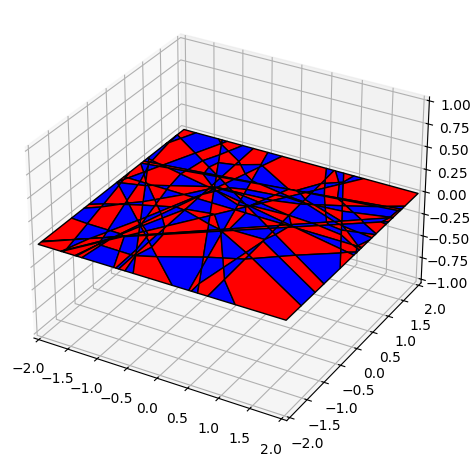
\includegraphics[width=\linewidth]{fig/ReLU-surface/initialization/quasi-homogeneous.png}
        \caption{With Biases}
    \end{subfigure}
    \begin{subfigure}{0.49\linewidth}
        \centering
        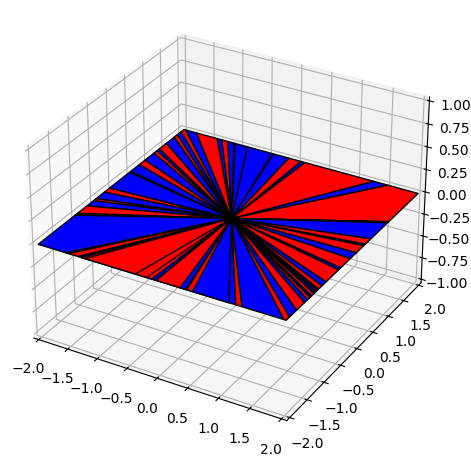
\includegraphics[width=\linewidth]{fig/ReLU-surface/initialization/homogeneous.png}
        \caption{Without Biases}
    \end{subfigure}
    \caption{\textbf{Surface of a ReLU network.}
    Here we depict the surface of a three-layer ReLU network $f(x;\theta) : \mathbb{R}^2 \to \mathbb{R}$ with twenty hidden units per layer at initialization, comparing configurations with biases (left) and without biases (right).
    %
    The network with biases partitions input space into convex polytopes that tile input space.
    %
    The network without biases partitions input space into convex conic sections emanating from the origin.
    %
    Each region exhibits a distinct activation pattern, allowing the partition to be colored with two colors based on the parity of active neurons.
    %
    The network operates linearly within each region and maintains continuity across boundaries.
    }
    \vspace{-20pt}
    \label{fig:relu-network-surface}
\end{wrapfigure}

\subsection{Surface of a piecewise linear network}
\label{app:nonlinear-surface}

The input-output map of a piecewise linear network $f(x;\theta)$, with $l$ hidden layers and $h$ hidden neurons per layer, is comprised of potentially $O(h^{dl})$ connected linear regions, each with their own vector of predictor coefficients \cite{raghu2017expressive}.
%
The exploration of this complex surface has been the focus of numerous prior works, the vast majority of them focused on counting and bounding the number of linear regions as a function of the width and depth \cite{pascanu2013number, montufar2014number, telgarsky2015representation, arora2016understanding, raghu2017expressive, serra2018bounding, hanin2019complexity, hanin2019deep}.
%
The central object in all of these studies is the \emph{activation region},
%
\begin{definition}
    For a piecewise linear network $f(x;\theta)$, comprising $N$ hidden neurons with pre-activation $z_i(x;\theta)$ for $i \in [N]$, let the \emph{activation pattern} $\mathcal{A}$ represent an assignment of signs $a_i \in \{-1,1\}$ to each hidden neuron.
    %
    The \emph{activation region} $\mathcal{R}(\mathcal{A};\theta)$ is the subset of input space that generates $\mathcal{A}$,
    \begin{equation}
        \mathcal{R}(\mathcal{A};\theta) = \{x \in \mathbb{R}^d \;|\; \forall i \;  a_iz_i(x;\theta) > 0\}.
    \end{equation}
\end{definition}

The input-output map is linear within each non-empty activation region and continuous at the boundary between regions.
%
Linearity implies that every non-empty\footnote{While it is trivial to see that for a network $f(x;\theta)$ with $N$ hidden neurons there are $2^N$ distinct activation patterns, not all activation patterns are attainable. See \citet{raghu2017expressive} for a discussion.} activation region is associated with a \emph{linear predictor} vector $\beta_{\mathcal{R}} \in \mathbb{R}^d$ such that for all $x \in R(\mathcal{A}; \theta)$, $\beta_\mathcal{R} = \nabla_x f(x;\theta)$.
%
Continuity implies that the boundary between regions is formed by a hyperplane determined by where the pre-activation for a neuron is exactly zero, $\{x : z_i(x;\theta) = 0\}$.
%
When the neighboring regions have different linear predictors\footnote{It is possible for neighboring regions to have the same linear predictor. Some works define linear regions as maximally connected component of input space with the same linear predictor \cite{hanin2019deep}.}, then this hyperplane is orthogonal to their difference, which is a vector in the span of the first-layer weights.
%
Taken together, this implies that the union of all activation regions forms a convex partition of input space, as shown in \cref{fig:relu-network-surface}.
%
We now present a surprisingly simple, yet to the best of our knowledge not previously understood property of this partition:

\begin{proposition}[2-colorable]
    If $f(x;\theta)$ lacks redundant neurons, implying that every neuron influences an activation region, then the partition of input space can be colored with two distinct colors such that neighboring regions do not share the same color.
\end{proposition}

The justification for this proposition is straightforward.
%
There is one color for regions with an even number of active neurons and another for regions with an odd number of active neurons.
%
Because $f(x;\theta)$ lacks redundant neurons, there does not exist a boundary between activation regions where two neurons activations change simultaneously.
%
In this work, we solely utilize this proposition for visualization purposes, as shown in \cref{fig:relu-network-surface}.
%
Nonetheless, we believe it may be of independent interest as it strengthens the connection between the surface of piecewise linear networks and the \emph{mathematics of paper folding}, a connection previously alluded to in the literature \cite{montufar2014number}.





\subsection{Dynamics of a two-layer piecewise linear network}
\label{app:nonlinear-two-layer}

We consider the dynamics of a two-layer piecewise linear network without biases, $f(x;\theta) = a^\intercal \sigma(W x)$, where $W \in \mathbb{R}^{h \times d}$ and $a \in \mathbb{R}^h$.
%
The activation function is $\sigma(z) = \max(z, \gamma z)$ for $\gamma \in [0,1)$, which includes ReLU $\gamma = 0$ and Leaky ReLU $\gamma \in (0,1)$.
%
We permit $h > d$, which in the limit as $h \to \infty$, ensures the network possesses the functional expressivity to represent any continuous nonlinear function from $\mathbb{R}^d$ to $\mathbb{R}$ passing through the origin.
%
Following a similar strategy used in \cref{sec:wide-deep-linear}, we consider the contribution to the input-output map from a single hidden neuron $k \in [h]$ with parameters $w_k \in \mathbb{R}^d$ and $a_k \in \mathbb{R}$.
%
As in the linear setting, each hidden neuron is associated with a conserved quantity, $\delta_k = \eta_w a_k^2 - \eta_a\|w_k\|^2$.
%
Unlike in the linear setting, this neuron's contribution to the output $f(x_i;\theta)$ is regulated by whether the input $x_i$ is in the neuron's \emph{active halfspace}, $\{x \in \mathbb{R}^d : w_k^\intercal x > 0\}$.
%
Let $C \in \mathbb{R}^{h \times n}$ be the matrix with elements $c_{ki} = \sigma'(w_k^\intercal x_i)$, which determines the activation of the $k^{\mathrm{th}}$ neuron for the $i^{\mathrm{th}}$ training data point.
%
The subgradient $\sigma'(z) = 1$ if $z > 0$, $\sigma'(z) \in [\gamma, 1]$ if $z = 0$, and $\sigma'(z) = \gamma$ if $z < 0$.
%
These activation functions exhibit positive homogeneity, implying $\sigma(z) = \sigma'(z) z$.
%
Thus, we can express $\sigma(w_k^\intercal x_i) = c_{ki}w_k^\intercal x_i$, allowing us to express the gradient flow dynamics for $w_k$ and $a_k$ as
\begin{equation}
    \label{eq:nonlinear-gradient-flow-a-w}
    \dot{a}_k = -\eta_a w_k^\intercal \left(\sum_{i=1}^nc_{ki}x_i\rho_i\right), \qquad \dot{w}_k = -\eta_w a_k \left(\sum_{i=1}^nc_{ki}x_i\rho_i\right),
\end{equation}
where $\rho_i = f(x_i;\theta) - y_i$ is the residual associated with the $i^{\mathrm{th}}$ training data point.
%
If we let $\beta_k = a_kw_k$, which determines the contribution of each hidden neuron to the output $f(x_i;\theta)$, then its not hard to see that the gradient flow dynamics of $\beta_k$ are
\begin{equation}
    \label{eq:nonlinear-gradient-flow-beta}
    \dot{\beta}_k = -\underbrace{\left(\eta_wa_k^2\mathbf{I}_d + \eta_aw_kw_k^\intercal\right)}_{M_k}\underbrace{\left(\textstyle\sum_{i=1}^nc_{ki}x_i\rho_i\right)}_{\xi_k}.
\end{equation}
As in the linear setting, the matrix $M_k \in \mathbb{R}^{d \times d}$ appears as a preconditioning matrix on the dynamics
%
Using the exact same derivation presented in \cref{app:single-neuron-beta}, whenever $a_k^2 \neq 0$, we can express $M_k$ entirely in terms of $\beta_k$ and $\delta_k$,
\begin{equation}
    M_k = \frac{\sqrt{\delta_k^2 + 4\eta_a\eta_w\|\beta_k\|^2} + \delta_k}{2}\mathbf{I}_d + \frac{\sqrt{\delta_k^2 + 4\eta_a\eta_w\|\beta_k\|^2} - \delta_k}{2}\frac{\beta_k\beta_k^\intercal}{\|\beta_k\|^2}.
\end{equation}
However, unlike in the linear setting, the vector $\xi_k \in \mathbb{R}^d$ driving the dynamics is not shared for all neurons because of its dependence on $c_{ki}$.
%
Additionally, the NTK matrix in this setting depends on $M_k$ and $C$, with elements $K_{ij} = \sum_{k = 1}^h c_{ki} x_i^\intercal \left(\eta_wa_k^2\mathbf{I}_d + \eta_aw_kw_k^\intercal\right) x_j c_{kj}$.
%
Thus, in order to assess the temporal dynamics of the NTK matrix, we must understand the dynamics of $M_k$ and $C$.
%
We consider a \emph{signed spherical coordinate} transformation separating the dynamics of $\beta_k$ into its directional $\hat{\beta}_k = \mathrm{sgn}(a_k)\tfrac{\beta_k}{\|\beta_k\|}$ and radial $\mu_k = \mathrm{sgn}(a_k)\|\beta_k\|$ components, such that $\beta_k = \mu_k \hat{\beta}_k$.
%
Here, $\hat{\beta}_k$ determines the orientation and direction of the halfspace where the $k^{\mathrm{th}}$ neuron is active, while $\mu_k$ determines the slope of the linear region in this halfspace.
%
These coordinates evolve according to,
%
\begin{equation}
    \dot{\mu}_k = -\sqrt{\delta_k^2 + 4\eta_a\eta_w\mu_k^2}\hat{\beta}_k^\intercal \xi_k, \qquad
    \dot{\hat{\beta}}_k = -\frac{\sqrt{\delta_k^2 + 4\eta_a\eta_w\mu_k^2} + \delta_k}{2\mu_k} \left(\mathbf{I}_d - \hat{\beta}_k\hat{\beta}_k^\intercal\right)\xi_k.
\end{equation}
%
These equations can be derived directly from \cref{eq:nonlinear-gradient-flow-a-w} through chain rule similar to \cref{app:single-neuron-mu-phi}.
%
In fact its worth noting that the this change of coordinates is similar to the change of coordinates used in the single-neuron analysis.
%
Expressed in terms of the parameters, $\hat{\beta}_k = \frac{w_k}{\|w_k\|}$ and $\mu_k = a_k \|w_k\|$.

% Derivation Details not provided:
% \begin{align}
%     \dot{\mu}_i &= \dot{a}_i \|w_i\| + a_i\dot{\|w_i\|}\\
%                 &= -\left(\eta_a\frac{\|w_i\|}{a_i} + \eta_w \frac{a_i}{\|w_i\|}\right)a_iw_i^\intercal \xi_i\\
%                 &= -\left(\eta_a\|w_i\|^2 + \eta_w a_i^2\right)\frac{a_iw_i}{a_i\|w_i\|}^\intercal \xi_i\\
%                 &= -\sqrt{\delta_i^2 + 4\eta_a\eta_w\mu_i^2}\hat{\beta}_i^\intercal \xi_i
% \end{align}
% where the last line uses the identity $\eta_w a_i^2 + \eta_a\|w_i\|^2 = \sqrt{\delta_i^2 + 4\eta_a\eta_w\mu_i^2}$ and the definition of $\hat{\beta}_i$.
% \begin{align}
%     \dot{\hat{\beta}}_i &= \dot{\left(\frac{w_i}{\|w_i\|}\right)}\\
%                 &= -\eta_w\frac{a_i}{\|w_i\|}\left(I - \frac{w_iw_i^\intercal}{\|w_i\|^2}\right)\xi_i
% \end{align}
% We now show how to express the prefactor $\eta_w\frac{a_i}{\|w_i\|}$ in terms of $\delta_i$ and $\mu_i$,
% \begin{align*}
%     \eta_w\frac{a_i}{\|w_i\|} &= \frac{\eta_a\eta_w 2a_i \|w_i\|}{2\eta_a\|w_i\|^2}\\
%     &= \frac{\eta_a\eta_w 2\mu_i}{(\eta_w a_i^2 + \eta_a\|w_i\|^2)
%  - (\eta_w a_i^2 - \eta_a\|w_i\|^2)}\\
%     &= \frac{\eta_a\eta_w 2\mu_i}{\sqrt{\delta_i^2 + \eta_a\eta_w4\mu_i^2} - \delta}\\
%     &= \frac{\sqrt{\delta_i^2 + \eta_a\eta_w4\mu_i^2} + \delta}{2\mu_i}
% \end{align*}
% Putting it all together gives us the expression for $\dot{\hat{\beta}}_i$.




\clearpage
\section{Experimental Details}
\label{app:experimental-details}
We used Google Cloud Platform (GCP) nodes to run all experiments. Figure 1 experiments were run on a node with 360 AMD Genoa CPU cores with runtime totaling approximately 90 minutes including averaging over seeds as described below. Neural network training and NTK calculation for Figure 5 was performed on single A100 GPU nodes. Runtime was approximately 20 hours for Figure 5(a), four hours for 5(b), 12 hours for 5(c) (with individual runs ranging from five to 30 minutes depending on the number of datapoints), and 12 hours for 5(d).  Figures 2, 3, and 4 are not compute-heavy, and these experiments were run on a personal computer. Overall, we estimate approximately 200 hours of single A100 runtime as well as 100 hours of the 360-core node accounting for failed runs and exploratory experiments.

\subsection{Figure 1: Teacher-Student with Two-layer ReLU Networks}
\label{app:experimental-details-two-layer}
For \cref{fig:two-layer-relu} we consider a student-teacher setup similar to that in \cite{chizat2019lazy}, with one-hidden layer ReLU networks of the form $f(x;\theta) = \sum_{i=1}^m a_i \sigma(w_i^\intercal x)$, where $f:\mathbb{R}^d\to\mathbb{R}$ and $\sigma$ is the ReLU activation function. The teacher model, $f^\mathrm{teacher}$, has $m=k$ hidden neurons initialized as $w^\mathrm{teacher}_i \overset{\text{i.i.d.}}{\sim} \mathrm{Unif}(S^{d-1})$ and $a_i \overset{\text{i.i.d.}}{\sim} \mathrm{Unif}(\{\pm1\})$ for $i \leq k$.
%sample $w_i \overset{\text{i.i.d.}}{\sim} \text{Unif}(\mathbb{S}^{d-1}(\frac{\tau}{\alpha}))$ and $a_i \overset{\text{i.i.d.}}{\sim} \{\pm\alpha\tau\}$
The student, $f^\mathrm{student}$, in turn, has $h$ hidden neurons. We use a symmetrized initialization, as considered in \cite{chizat2019lazy}, where for $i \leq h/2$, we sample $w_i \overset{\text{i.i.d.}}{\sim} S^{d-1}$ and $a_i \overset{\text{i.i.d.}}{\sim} \mathrm{Unif}(\{\pm1\})$, and then for $i \geq \frac{h}{2} + 1$ we symmetrize by setting $w_i = w_{i - h/2}$ and $a_i = -a_{i - h/2}$. This ensures that $f^\mathrm{student}$ predicts 0 on any input at initialization.

Note that the \textit{base} student initialization described thus far is perfectly balanced at each neuron, that is $\delta_i = 0$ for $i \in [m]$; we also define this to be our setting where the scale $\tau$ is 1. In order to transform the base initialization into a particular setting of $\tau$ and $\delta$, we first solve for the relative layer scaling $\alpha$ in $\delta^2 = \tau^2 (\alpha^2 - \alpha^{-2})$ and then scale each $w_i$ by $\tau/\alpha$ and each $a_i$ by $\tau\alpha$.
%
We obtain a training dataset $\{x^{(i)}, y^{(i)}\}_{i=1}^n$ by sampling $x^{(i)} \overset{\text{i.i.d.}}{\sim} S^{d-1}$ and computing noiseless labels as $y^{(i)} = f^\mathrm{teacher}(x^{(i)};\theta^\mathrm{teacher})$. The student is then trained with full-batch gradient descent on a mean square loss objective.

\textbf{Figure 1 (a).}

Here the setting is: $d=2$, $h=50$, $k=3$, and $n=20$. We sample a single teacher and then train four students with the same base initialization but different configurations of $\tau$ and $\delta$: $(\tau=0.1, \delta=0)$ and $(\tau=2, \delta=0)$ for the left subfigure, and $(\tau=0.1, \delta=1)$ and $(\tau=0.1, \delta=-1)$ for the right subfigure. Training is for 1 million steps at a learning rate of 1e-4.

\textbf{Figure 1 (b).}

Here the setting is: $d=100$, $m=50$, $k=3$, and $n=1000$, as in Fig. 1c of \cite{chizat2019lazy}. Training is performed with learning rate of 5e-3$/\tau^2$. Test error is computed as mean square error over a held-out set of 10,000 datapoints.
%
We sweep over $\tau$ over a logarithmic scale in the range $[0.1, 2]$ and $\delta$ over a linear scale in the range $[-1, 1]$. We average over 16 random seeds, where the seed controls the sampling of: the teacher weights $\theta^\mathrm{teacher}$, the base initialization of $\theta^\mathrm{student}$, and the training data $\{x^{(i)}\}_{i=1}^n$. In this way, each random seed is used for a sweep over all combinations of $\tau$ and $\delta$ in the sweep; we simply apply the scaling described above to get to each point on the $(\tau, \delta)$ grid.
%
The kernel distance computed is as defined in \cite{fort2020deep}, where here we compute it at time $t$ relative to the kernel at initialization, i.e. $S(t) = 1 - \langle K_{0}, K_{t}\rangle / \left(\|K_{0}\|_F\|K_{t}\|_F\right)$. In \cref{fig:two-layer-supporting}, we additionally plot Hamming and parameter distances relative to initialization, as well as training loss, while training for ten times longer than in \cref{fig:two-layer-relu} (b).

Notebooks generating all two-layer experiment figures are provided \href{https://github.com/allanraventos/getrichquick/blob/main/two-layer-relu}{here}.

\begin{figure}[H] 
    \centering
    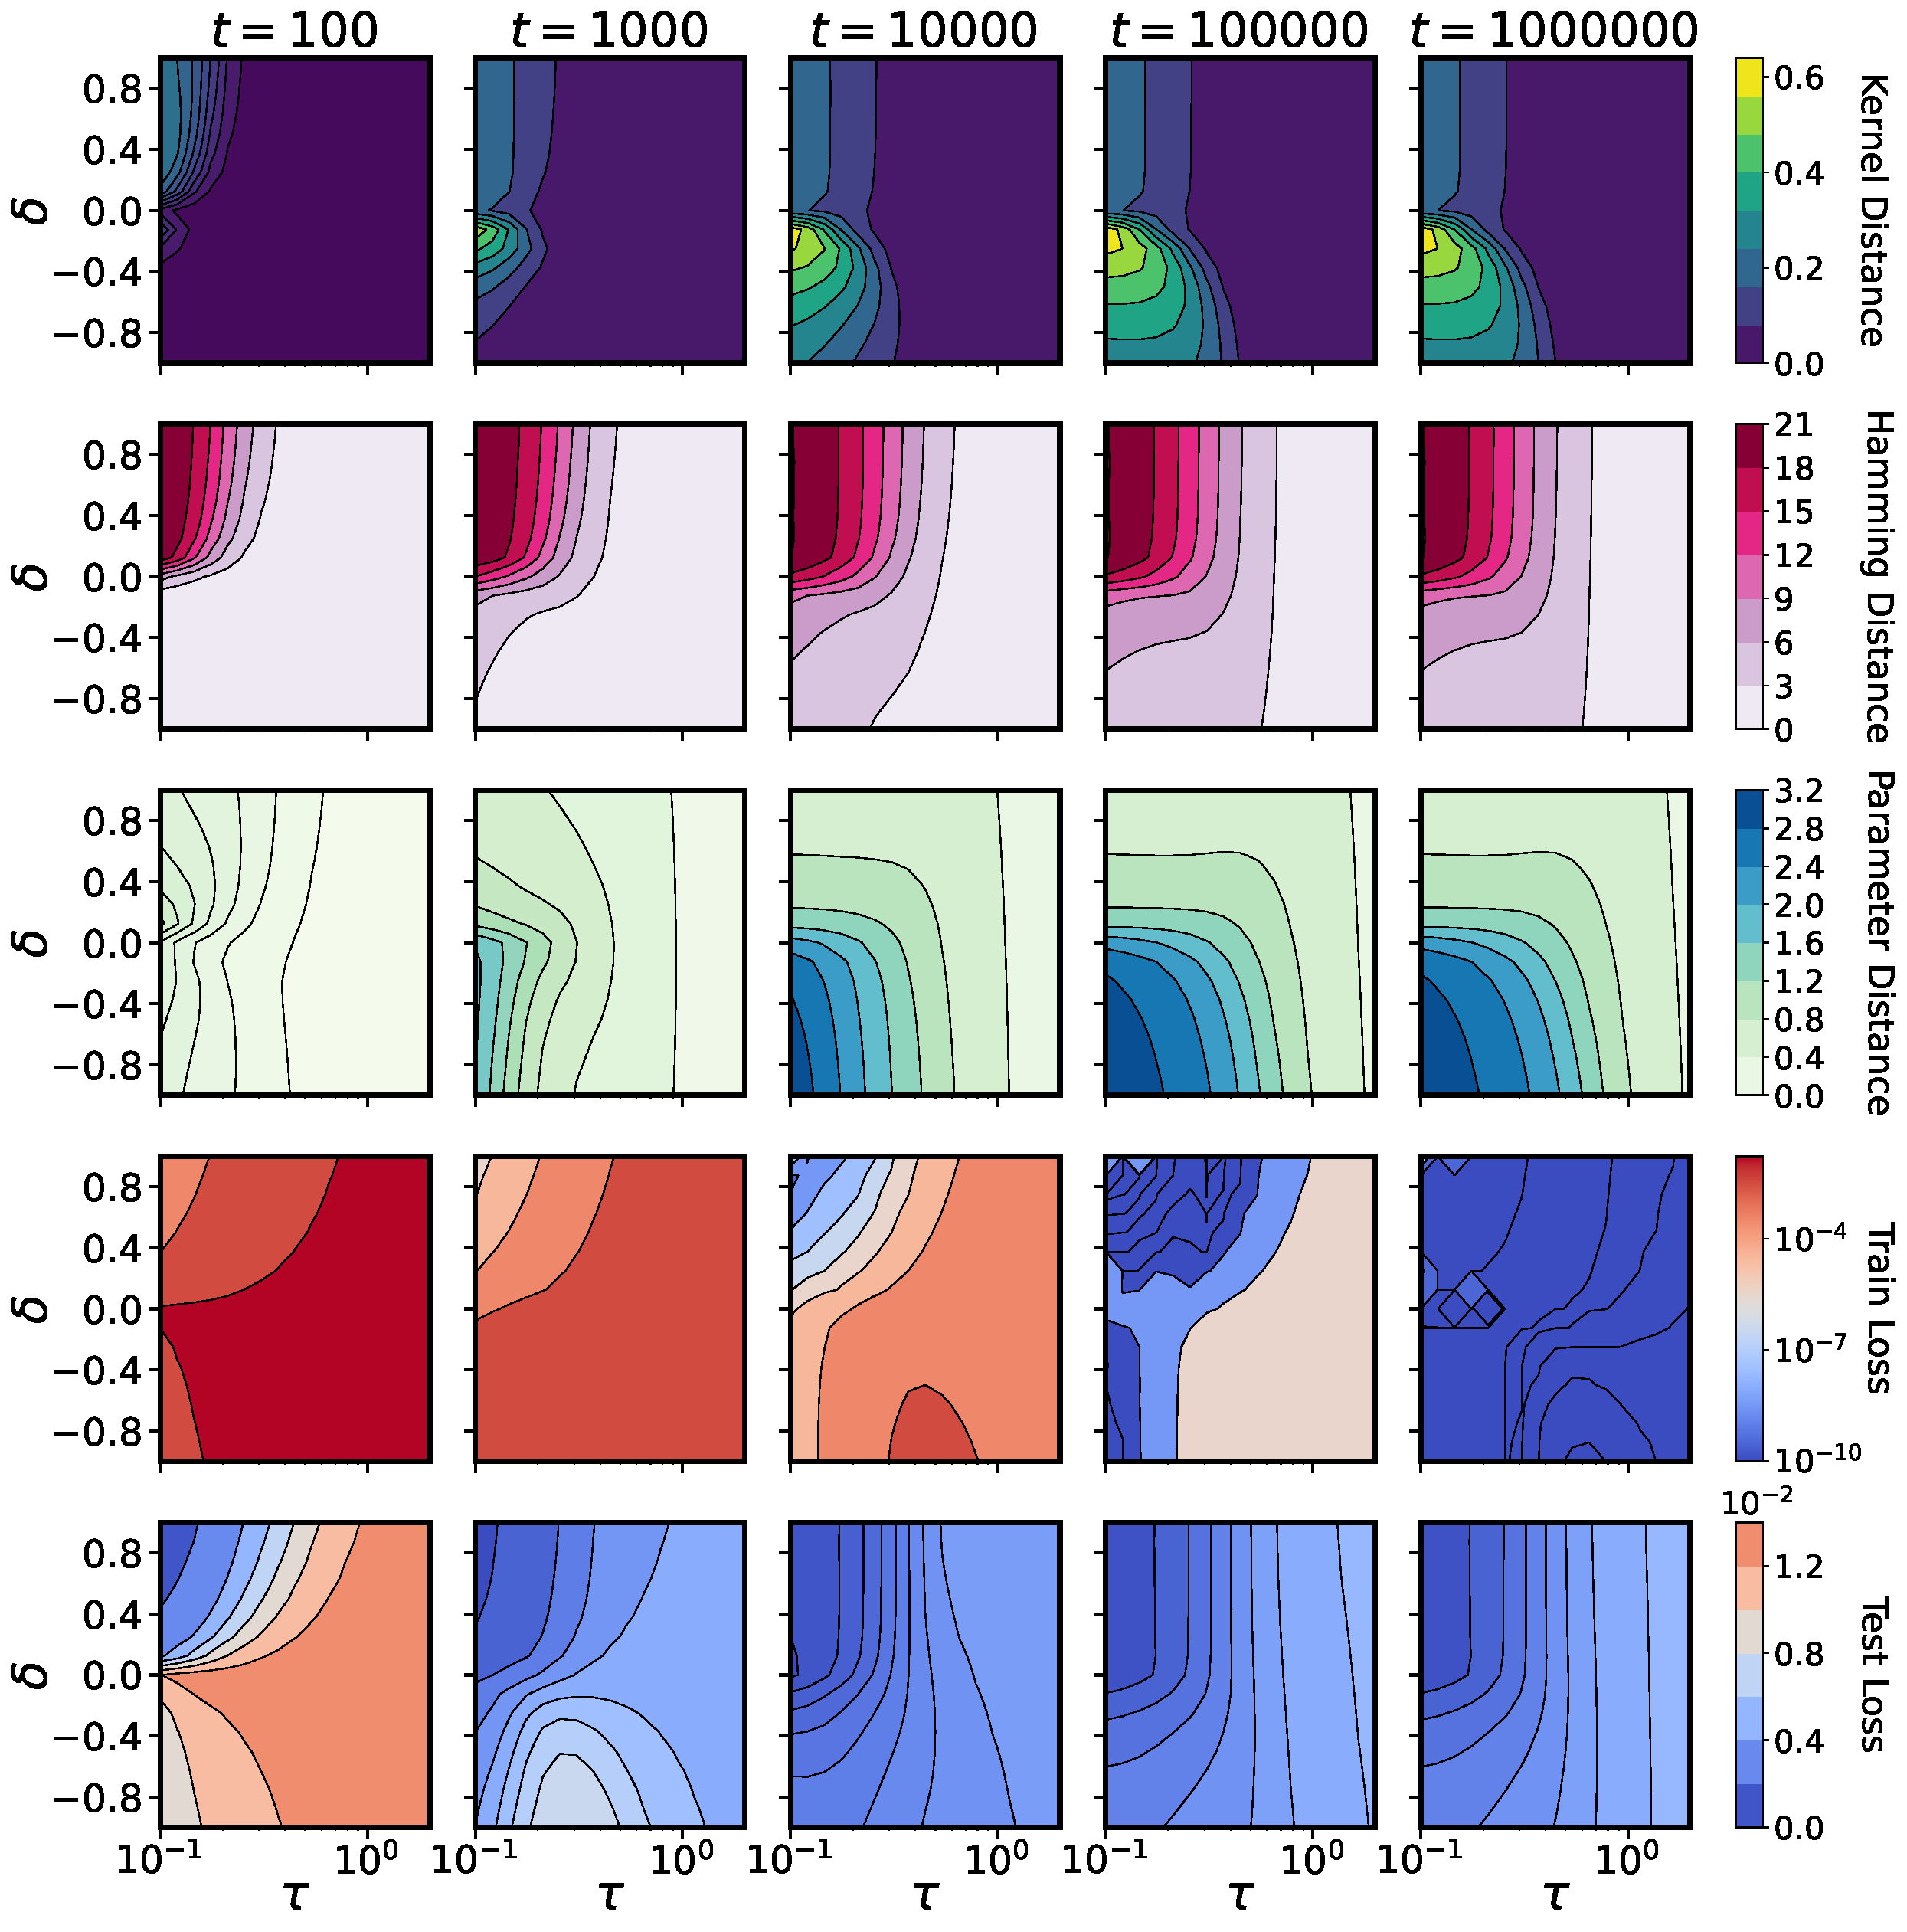
\includegraphics[width=\columnwidth]{fig/two-layer/supporting_other_v3.pdf}
    \caption{\textbf{Supporting figures for \cref{fig:two-layer-relu} (b).} We plot Hamming distance, parameter distance, and training loss, on top of the test loss and kernel distance considered in \cref{fig:two-layer-relu} (b), and train for ten times longer than in \cref{fig:two-layer-relu} (b). We observe that although training loss still drops between $10^5$ and $10^6$ steps, the test loss and other distances considered remain largely unchanged. Training loss is saturated at 1e-10.}
    \label{fig:two-layer-supporting}
\end{figure}

\subsection{Figures 2, 3, 4: Single-Neuron Linear Network}
\label{app:experimental-details-single-neuron}

Figures 2, 3, and 4 were generated by simulating gradient flow using  \texttt{scipy.integrate.solve\_ivp} function with the RK45 method for solving the ODEs, with a relative tolerance of $1 \times 10^{-6}$ and time span of $(0,20)$.
%
In the experiments with full-rank data, we used $X^\intercal X = \mathbf{I}_2$, $\beta_* = \left[\begin{smallmatrix} 0 \\ 1 \end{smallmatrix}\right]$, and $\beta_0 = \left[\begin{smallmatrix} -1 \\ 0 \end{smallmatrix}\right]$. 
%
For the experiment with low-rank data, we used $X^\intercal X = \left[\begin{smallmatrix} 0.25 & 0.5 \\ 0.5 & 1 \end{smallmatrix}\right]$, $\beta_* = \left[\begin{smallmatrix} 0.44 \\ 0.88 \end{smallmatrix}\right]$, and $\beta_0 = \left[\begin{smallmatrix} 0.4 \\ 0.05 \end{smallmatrix}\right]$.
%
See the discussion in \cref{app:single-neuron-exact-solutions} for details on how we determined our theoretical predictions.
%
A notebook generating all the figures is provided \href{https://github.com/allanraventos/getrichquick/blob/main/single-neuron/Single_Neuron.ipynb}{here}.


\subsection{Figure 5: }
\label{app:fig-5}

\textbf{Kernel Distance}

We trained LeNet-5~\cite{lecun1998gradient} (with ReLU nonlinearity and Max Pooling) on MNIST~\cite{lecun1998gradient}. We use He initialization~\cite{he2015delving} and divide the first layer weights by $\alpha$ and multiply the last layer weights by $\alpha$ at initialization, which keeps the network functionally the same at initialization. We trained the model for 500 epochs with a learning rate of 1e-4 and a batch size of 512. The parameter distance is defined as the $L_2$ distance between all the parameters. To quantify the distance between the activations, we binarize the hidden activation with 1 representing an active neuron. We evaluate Hamming distance over all the binarized hidden activations normalized by the the total number of the activations. We use kernel distance \cite{fort2020deep}, defined as
$S(t_1,t_2) = 1 - \langle K_{t_1}, K_{t_2}\rangle / \left(\|K_{t_1}\|_F\|K_{t_2}\|_F\right)$, which is a scale invariant measure of similarity between the NTK at two points in time. We subsample 10\% of MNIST to evaluate the Hamming distance and kernel distance. All curves in the figure are averaged over 8 runs.

\textbf{Gabor Filters}

We are training a small ResNet based on the CIFAR10 script provided in the DAWN benchmark (code available \href{https://github.com/davidcpage/cifar10-fast}{here}).
The only modifications to the provided code base are we increase the convolution kernel size from $3 \times 3$ to $15 \times 15$, to better observe the learned spatial patterns, and we set the weight decay parameter to $0$ to avoid confounding variables.
Moreover, we are dividing the convolutional filters weights by a parameter $\alpha$ (after standard initialization) which controls the balancedness of the network.
To quantify the smoothness of the filters, we compute the normalized Laplacian of each filter $w_{ij} \in \mathbb{R}^{15 \times 15}$, over input $i=(1, 2, 3)$ and output $j=(1, ..., 64)$ channels
\begin{equation}\label{eq:laplacian}
    \text{smoothness}(w_{ij}) := \left\lVert\frac{w_{ij}}{\|w_{ij}\|_2} \ast \Delta \right\rVert_2^2
\end{equation}
where the Laplacian kernel is defined as
\begin{equation}
    \Delta := \left(\begin{array}{ccc}
         -0.25 & -0.5 & -0.25\\
         -0.5 & 2 & -0.5 \\
         -0.25 & -0.5 & -0.25
    \end{array}\right).
\end{equation}

\begin{figure}[H]
    \begin{subfigure}{0.535\textwidth}
        \centering
        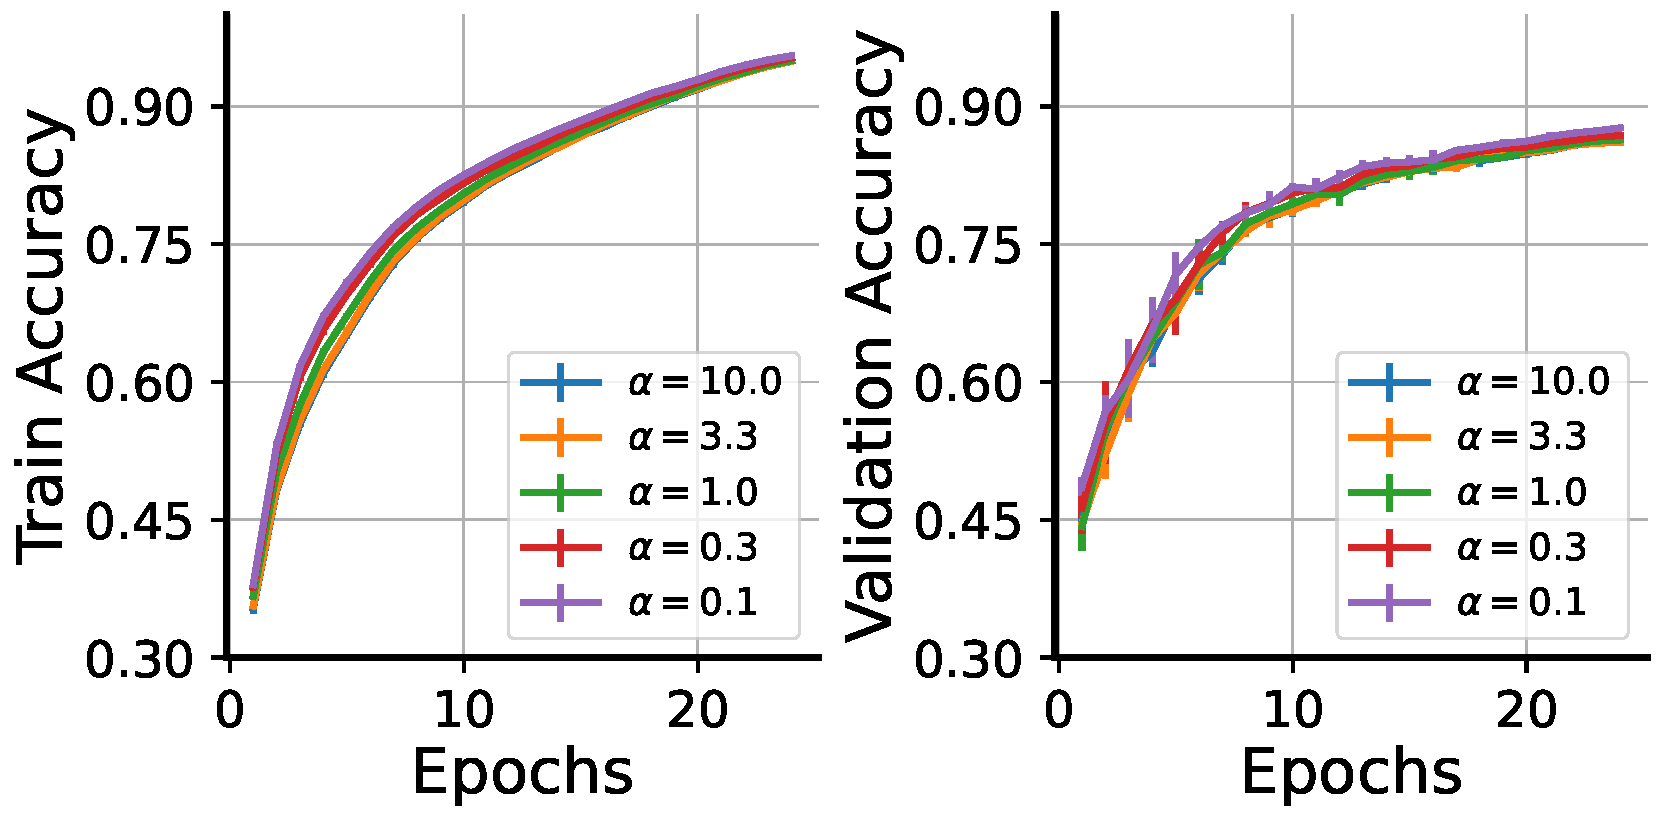
\includegraphics[width=\linewidth]{fig/deep-networks/gabors/gabors_accuracy.pdf}
        \caption{Accuracy}
    \end{subfigure}
    \begin{subfigure}{0.455\textwidth}
        \centering
        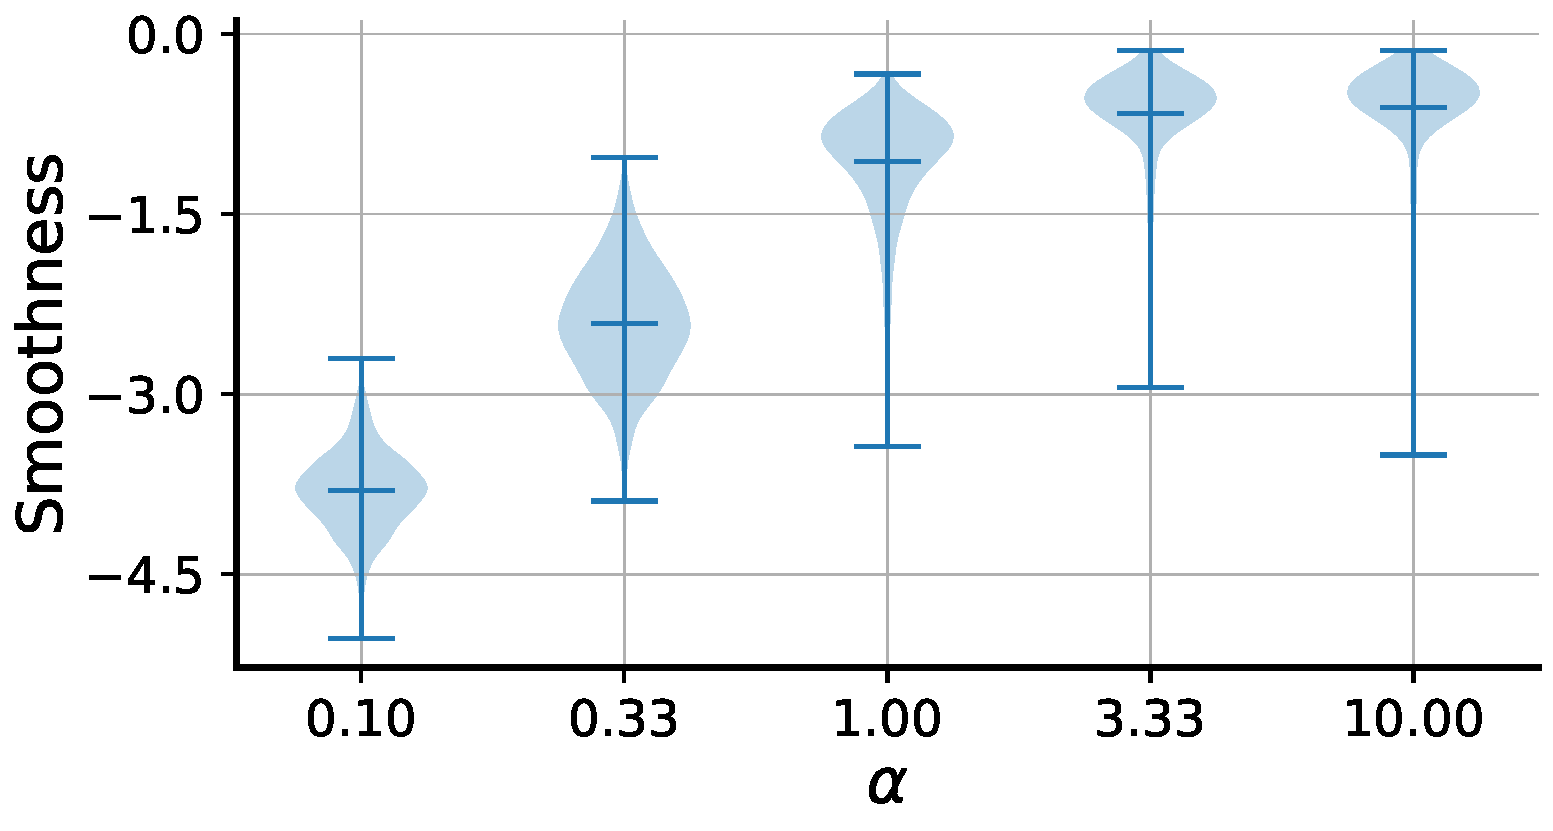
\includegraphics[width=\linewidth]{fig/deep-networks/gabors/gabor_smoothness.pdf}
        \caption{Gabor Smoothness}
    \end{subfigure}
    \caption{\textbf{Interpreting convolutional filters.}
    CNN experiments on CIFAR10. We can see in \textbf{A)} that all networks achieve comparable training and test accuracy, despite the modification in initialization. However, in \textbf{B)} we see that networks with a small initialization ($\alpha<1$) learn much smoother filters, giving quantiative support to results in Fig.~\ref{fig:deep-network}. The smoothness is defined as the normalized Laplacian of the filters (see text, eq.~\ref{eq:laplacian}).
    }
    \label{fig:gabors}
\end{figure}

\textbf{Random Hierarchy Model}

We refer to \cite{petrini2023deep}, who originally proposed the random hierarchy model (RHM) as a tool for studying how deep networks learn compositional data, for a more in-depth treatment. Here we briefly recap the setup following the notation used in \cite{petrini2023deep}.

An RHM essentially lets us build a random classification task with a clear hierarchical structure. The top level of the RHM specifies $m$ equivalent high-level features for \textit{each} class label in $\{1,\ldots,n_c\}$, where each feature has length $s$ and $n_c$ is the number of classes. For example, suppose the vocabulary at the top level is $\mathcal{V}_L=\{a, b, c\}$, $n_c = 2$, $m=3$, and $s=2$. Then in a particular instantiation of this RHM, we might have that Class 1 has $ab$, $aa$, and $ca$ as equivalent high-level features (this is precisely the example used in Fig.1 of \cite{petrini2023deep}). Class 2 will then have three random high-level features, with the constraint that they are \textbf{not} features for Class 1, for example, $bb, bc, ac$.

Each successive level specifies $m$ equivalent lower-level features for each ``token" in the vocabulary at the previous level. For example, if $\mathcal{V}_{L-1}=\{d,e,f\}$, we might have that $a$ can be equivalently represented as $de$, $df$, or $ff$; $b$ and $c$ will each have $m$ equivalent representations of their own. We assume that the vocabulary size, $v$, is the same at all levels. Therefore, sampling an RHM with hyperparameters $n_c, m, s, v$ requires sampling $m n_c + (L-1) m v$ rules.

In order to sample a datapoint from an RHM, we first sample a class label (e.g. Class 1), then uniformly sample one of the highest level features, (e.g. $ab$), then for each ``token" in this feature we sample lower level features (e.g. $a \to de$, $b \to ee$), and so on recursively. The generated sample will therefore have length $s^L$ and a class label. For training a neural network to perform this classification task, each input is converted into a one-hot representation, which will be of shape $(s^L, v)$, and is then flattened.
 
We use the code released by \cite{petrini2023deep} to train an MLP of width 64 with three hidden layers to learn an RHM with $L=3$, $n_c=8, m=4, s=2, v=8$. The main change we make is allowing for scaling the initialization of the first layer by $1/\alpha$ and the initialization the readout layer by $\alpha$. We then sweep over $\alpha \in \{0.03, 0.1, 0.3, 1, 3, 10\}$ and over the number of datapoints in the training set, which is specified as a fraction of the total number of datapoints the RHM can generate. We average test accuracy, which is by default computed on a held-out set of 20,000 samples, over six random seed configurations, where each configuration seeds the RHM, the neural network, and the data generation. 

We train with the default settings used in \cite{petrini2023deep}, that is stochastic gradient descent with momentum of 0.9, run for 250 epochs with a learning rate initialized at 6.4 (0.1 times width) and decayed with a cosine schedule down to 80\% of epochs. The batch size of 128; we do not use biases or weight decay.

\textbf{Grokking}

We are training a one layer transformer model on the modular arithmetic task in \citet{power2022grokking}.
Our experimental code is based on an existing Pytorch implementation (code available \href{https://github.com/teddykoker/grokking}{here}).
The only modifications to the provided code base is that we use a single transformer layer (instead of the default 2-layer model).
Prior analysis in \citet{nanda2023progress} has shown that this model can learn a minimal (attention-based) circuit that solves the task.

We study the effects on grokking time (defined as $\geq0.99$ accuracy on the validation data) of two manipulations.
Firstly, we divide the embedding weights of the positional and token embeddings by the same balancedness parameter $\alpha$ as in the CNN gabor experiments.
Secondly, like in \citet{kumar2023grokking}, we multiply the output of the model (i.e., the logits) by a factor $\tau$ and divide the learning rate by $\tau^2$.

\begin{figure}[H]
    \begin{subfigure}{0.49\textwidth}
        \centering
        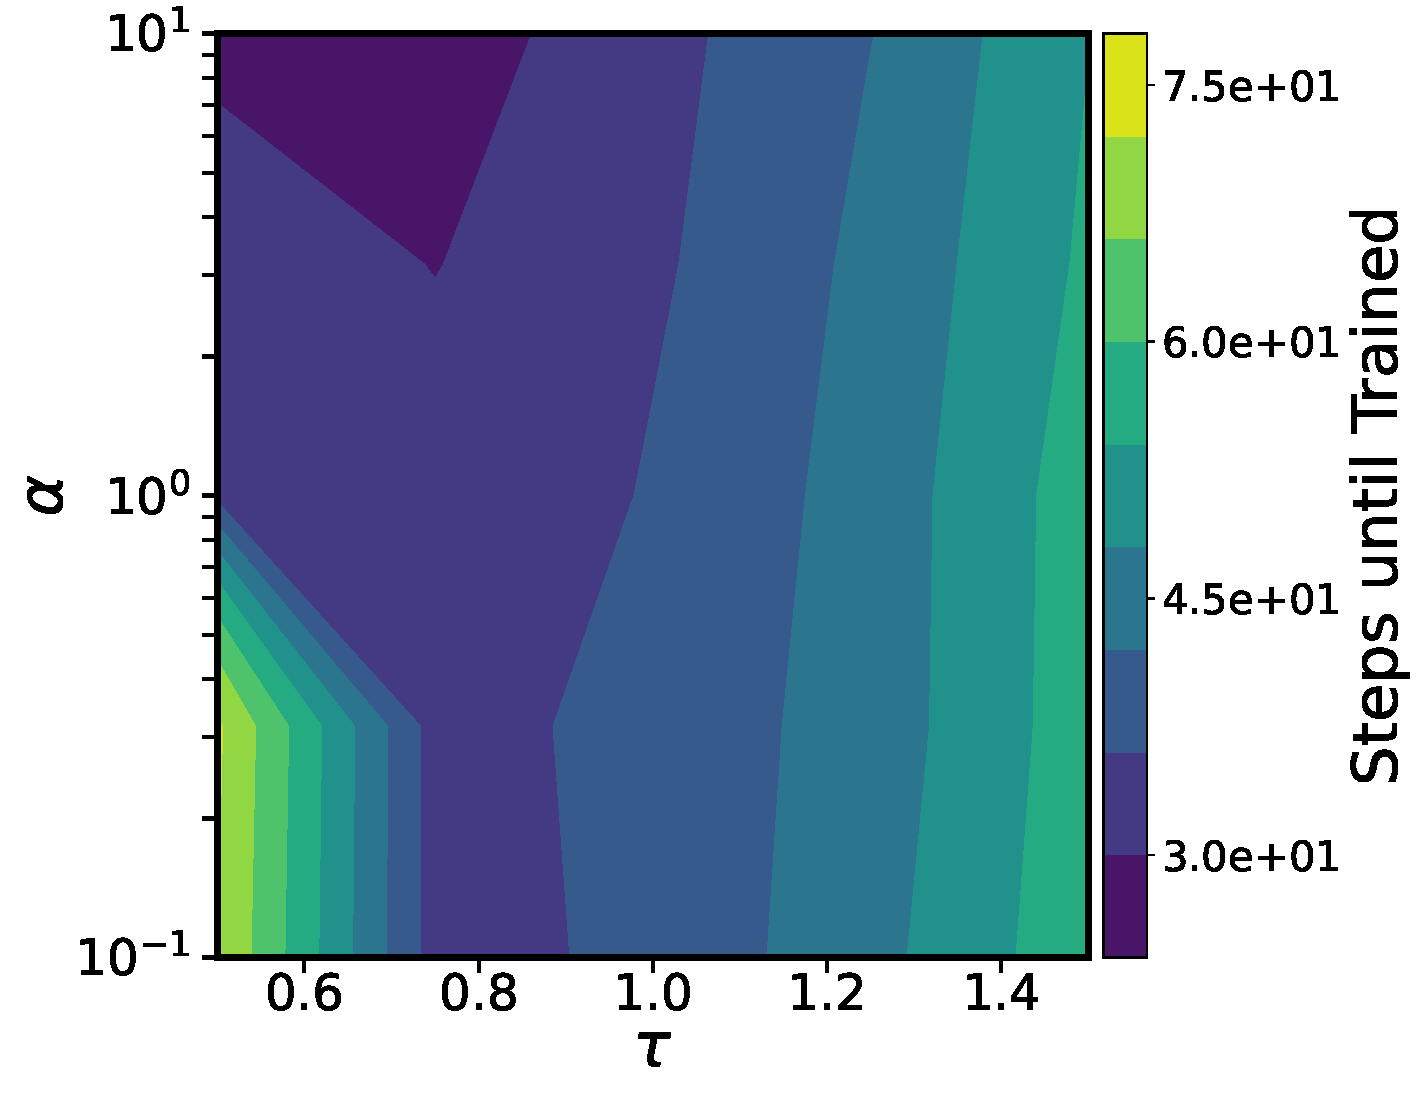
\includegraphics[width=\linewidth]{fig/deep-networks/grokking/grok_trained.pdf}
        \caption{Steps until training}
    \end{subfigure}
    \begin{subfigure}{0.49\textwidth}
        \centering
        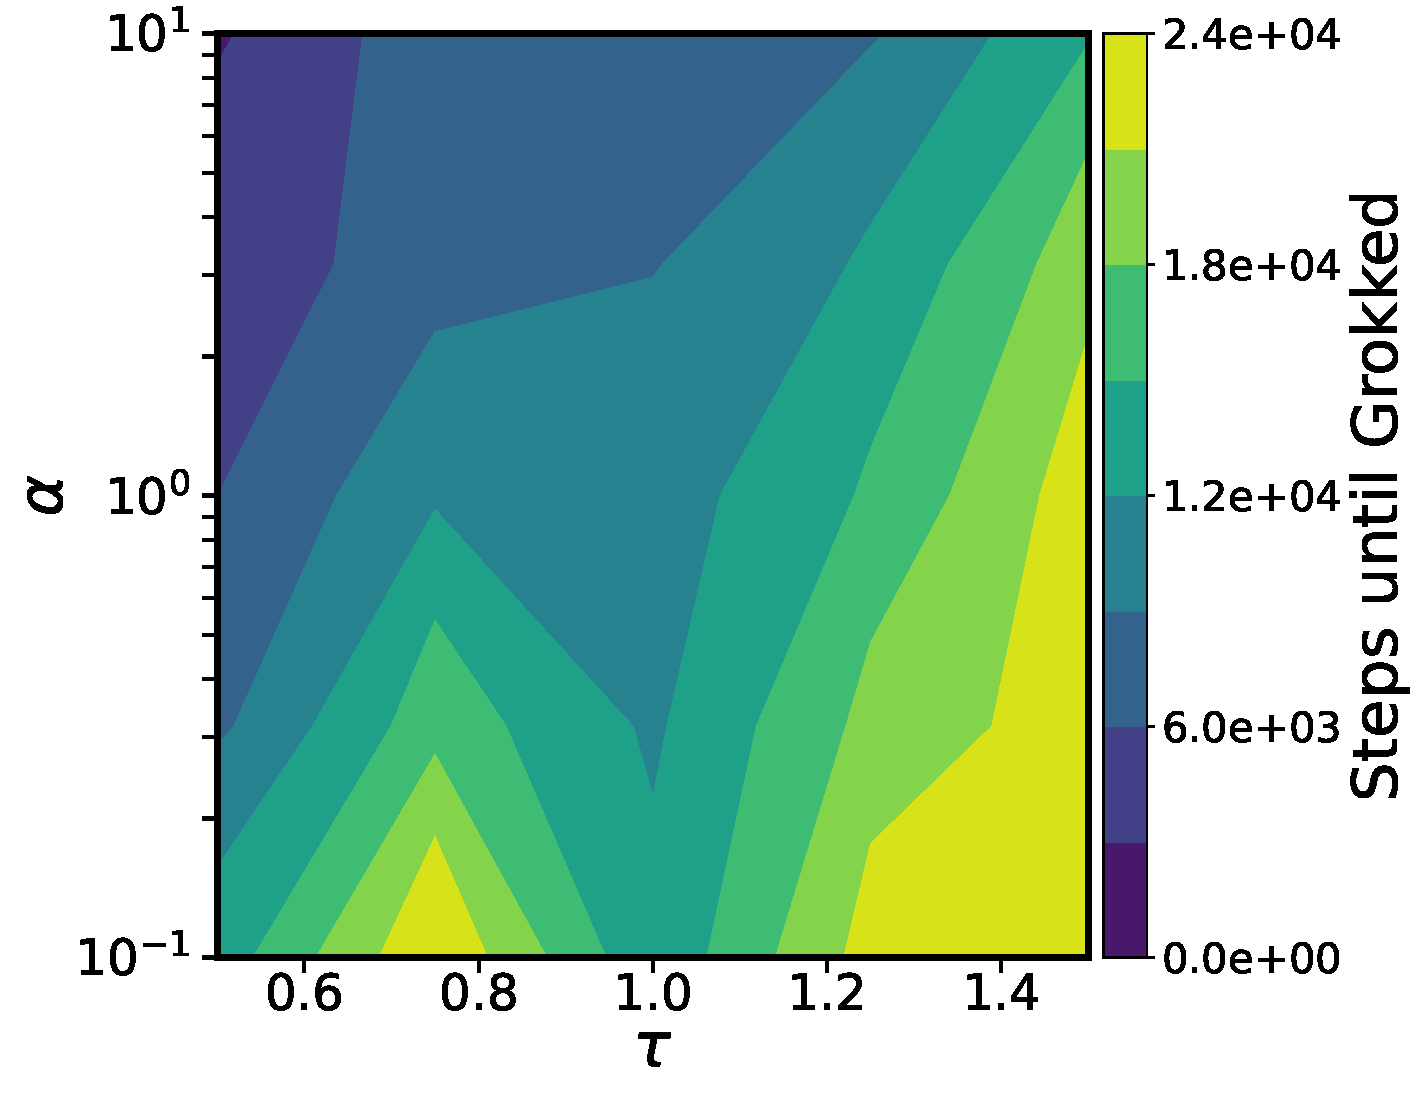
\includegraphics[width=\linewidth]{fig/deep-networks/grokking/grok_grokked.pdf}
        \caption{Steps until grokked}
    \end{subfigure}
    \caption{\textbf{Transformer Grokking in Modular Arithmetic Task.}
    \textbf{A)} Shows the number of training steps required until the training accuracy passes a predefined threshold of $99\%$; we sample scaling $\tau \in \{0.5, 0.75, 1.0, 1.25, 1.5 \}$ \citep{kumar2023grokking} and balance $\alpha \in \{0.1, 0.3, 1.0, 3.0, 10 \}$ on a regular grid over $n=5$ random initializations with a maximal computational budget of $m=30,000$ training steps.
    \textbf{B)} Same as \textbf{A)}, but reporting the number of training steps required until the test performance passes the predefined threshold of $99\%$. We clearly see the fastest grokking in an unbalanced rich setting.
    }
    \label{fig:grokking}
\end{figure}





\end{document}